\documentclass[twoside,symmetric,notoc]{tufte-book} 
 
\usepackage[normalem]{ulem}
 
% Margins
\geometry{
  left=1in, % left margin
  bottom=1in,
  textwidth=25pc, % main text block
  marginparsep=1.5pc, % gutter between main text block and margin notes
  marginparwidth=13pc % width of margin notes
}

% Character spacing and hyphenating
\usepackage{microtype}
\usepackage[none]{hyphenat}
\sloppy

% Links
\usepackage{url}
\usepackage{hyperref}
\usepackage[dvipsnames]{xcolor}
\newcommand\myshade{85}
\colorlet{myurlcolor}{MidnightBlue}
\hypersetup{
    colorlinks=true,
    linkcolor=myurlcolor!\myshade!black,
    urlcolor=myurlcolor!\myshade!black,
}
\PassOptionsToPackage{hyphens}{url}

% Figures
\usepackage{graphicx} 
\graphicspath{{graphics/}}
\setkeys{Gin}{width=\linewidth,totalheight=\textheight,keepaspectratio}
\usepackage{mwe}
\usepackage{subfig}

% Tables
\usepackage{color, colortbl}
\definecolor{Gray}{gray}{0.9}
\usepackage{booktabs}

% Math
\usepackage{amsfonts}
\usepackage{amssymb}
\usepackage{amsmath}
\usepackage{wasysym}

% Code
\usepackage{minted}
\usemintedstyle{vs}

% Verbatim
\usepackage{fancyvrb}
\fvset{fontsize=\normalsize} 

% Commands for i.e. and e.g.
\usepackage{xspace}
\newcommand{\hairsp}{\hspace{1pt}} 
\newcommand{\ie}{\textit{i.\hairsp{}e.,}\hspace{3pt}}
\newcommand{\eg}{\textit{e.\hairsp{}g.,}\hspace{3pt}} 
\newcommand{\etal}{\textit{et al.}\xspace}

% Macros for typesetting the documentation
\newcommand{\hangleft}[1]{\makebox[0pt][r]{#1}}
\newcommand{\hquad}{\hskip0.5em\relax}% half quad space
\newcommand{\na}{\quad--}% used in tables for N/A cells
\providecommand{\XeLaTeX}{X\lower.5ex\hbox{\kern-0.15em\reflectbox{E}}\kern-0.1em\LaTeX}
\newcommand{\tXeLaTeX}{\XeLaTeX\index{XeLaTeX@\protect\XeLaTeX}}
% \index{\texttt{\textbackslash xyz}@\hangleft{\texttt{\textbackslash}}\texttt{xyz}}
\newcommand{\tuftebs}{\symbol{'134}}% a backslash in tt type in OT1/T1
\newcommand{\doccmdnoindex}[2][]{\texttt{\tuftebs#2}}% command name -- adds backslash automatically (and doesn't add cmd to the index)
\newcommand{\doccmddef}[2][]{%
  \hlred{\texttt{\tuftebs#2}}\label{cmd:#2}%
  \ifthenelse{\isempty{#1}}%
    {% add the command to the index
      \index{#2 command@\protect\hangleft{\texttt{\tuftebs}}\texttt{#2}}% command name
    }%
    {% add the command and package to the index
      \index{#2 command@\protect\hangleft{\texttt{\tuftebs}}\texttt{#2} (\texttt{#1} package)}% command name
      \index{#1 package@\texttt{#1} package}\index{packages!#1@\texttt{#1}}% package name
    }%
}% command name -- adds backslash automatically
\newcommand{\doccmd}[2][]{%
  \texttt{\tuftebs#2}%
  \ifthenelse{\isempty{#1}}%
    {% add the command to the index
      \index{#2 command@\protect\hangleft{\texttt{\tuftebs}}\texttt{#2}}% command name
    }%
    {% add the command and package to the index
      \index{#2 command@\protect\hangleft{\texttt{\tuftebs}}\texttt{#2} (\texttt{#1} package)}% command name
      \index{#1 package@\texttt{#1} package}\index{packages!#1@\texttt{#1}}% package name
    }%
}% command name -- adds backslash automatically
\newcommand{\docopt}[1]{\ensuremath{\langle}\textrm{\textit{#1}}\ensuremath{\rangle}}% optional command argument
\newcommand{\docarg}[1]{\textrm{\textit{#1}}}% (required) command argument
\newenvironment{docspec}{\begin{quotation}\ttfamily\parskip0pt\parindent0pt\ignorespaces}{\end{quotation}}% command specification environment
\newcommand{\docenv}[1]{\texttt{#1}\index{#1 environment@\texttt{#1} environment}\index{environments!#1@\texttt{#1}}}% environment name
\newcommand{\docenvdef}[1]{\hlred{\texttt{#1}}\label{env:#1}\index{#1 environment@\texttt{#1} environment}\index{environments!#1@\texttt{#1}}}% environment name
\newcommand{\docpkg}[1]{\texttt{#1}\index{#1 package@\texttt{#1} package}\index{packages!#1@\texttt{#1}}}% package name
\newcommand{\doccls}[1]{\texttt{#1}}% document class name
\newcommand{\docclsopt}[1]{\texttt{#1}\index{#1 class option@\texttt{#1} class option}\index{class options!#1@\texttt{#1}}}% document class option name
\newcommand{\docclsoptdef}[1]{\hlred{\texttt{#1}}\label{clsopt:#1}\index{#1 class option@\texttt{#1} class option}\index{class options!#1@\texttt{#1}}}% document class option name defined
\newcommand{\docmsg}[2]{\bigskip\begin{fullwidth}\noindent\ttfamily#1\end{fullwidth}\medskip\par\noindent#2}
\newcommand{\docfilehook}[2]{\texttt{#1}\index{file hooks!#2}\index{#1@\texttt{#1}}}
\newcommand{\doccounter}[1]{\texttt{#1}\index{#1 counter@\texttt{#1} counter}}


% Document parameters
\titleformat{\chapter}[hang] 
{\normalfont\huge}{ \thechapter}{1em}{} 
\titleformat*{\section}{\itshape\LARGE\bfseries}
\titleformat*{\subsection}{\itshape\Large\bfseries}

\makeatletter
\g@addto@macro{\UrlBreaks}{\UrlOrds}
\makeatother

% List of figures
\makeatletter
\renewcommand*\l@figure{\@dottedtocline{1}{1.5em}{2.3em}}
\makeatother

% List of tables
\makeatletter
\renewcommand*\l@table{\@dottedtocline{1}{1.5em}{2.3em}}
\makeatother

% Abstract
\def\abstractpage{\clearpage
  \newgeometry{left=1in,right=1in}
  \begin{center}
    University of Washington \\
    \vspace{0.2in}
    \textbf{Abstract} \\
    \vspace{0.2in}
    The Use of Automatic Identification System Data to Determine Appropriate Stand-On Vessel Maneuvers \\
    \vspace{0.2in}
    Maureen K. Rowell \\
    \vspace{0.20in}
    Co-Chairs of the Supervisory Committee:\\
    Anne Goodchild, Ed McCormack\\
    Civil Engineering\\
    \end{center}
    \doublespacing
}

\def\endabstractpage{
  \restoregeometry
  \newpage
}
% Appendix
\usepackage[most]{tcolorbox}

% References
%\usepackage{natbib}

% Glossary
\usepackage[acronym,nomain,nonumberlist]{glossaries}
\makeglossaries
\newacronym{arpa}{ARPA}{Automatic Radar Plotting Aid}
\newacronym{ais}{AIS}{Automatic Identification System}
\newacronym{cog}{COG}{Course over ground}
\newacronym{colregs}{COLREGS}{International Regulations for Preventing Collisions at Sea}
\newacronym{cpa}{CPA}{Closest Point of Approach}
\newacronym{ecdis}{ECDIS}{Electronic Chart Display and Information System}
\newacronym{imo}{IMO}{International Maritime Organization}
\newacronym{ism}{ISM}{International Safety Management}
\newacronym{maib}{MAIB}{Marine Accident Investigation Branch, U.K.}
\newacronym{met}{MET}{Marine Education and Training}
\newacronym{mmsi}{MMSI}{Maritime Mobile Service Identity}
\newacronym{ntsb}{NTSB}{National Transportation Safety Board}
\newacronym{opa}{OPA}{Oil Pollution Act}
\newacronym{pawss}{PAWSS}{Ports and Waterways Safety System}
\newacronym{pwsa}{PWSA}{Ports and Waterways Safety Act}
\newacronym{sms}{SMS}{Safety Management System}
\newacronym{sog}{SOG}{Speed over ground}
\newacronym{solas}{SOLAS}{Safety of Life at Sea}
\newacronym{tss}{TSS}{Traffic Separation Scheme}
\newacronym{unclos}{UNCLOS}{United Nations Convention for the Law of the Sea}
\newacronym{uscg}{USCG}{United States Coast Guard}
\newacronym{vts}{VTS}{Vessel Traffic Service}


\newglossaryentry{give-way vessel}
{
    name=give way,
    description={The vessel must stay out of the way of the stand-on vessel and avoid crossing ahead of its bow}
}
\newglossaryentry{stand-on vessel}
{
    name=stand-on vessel,
    description={The vessel is to keep its course and speed}
}
\newglossaryentry{ownship}
{
    name=ownship,
    description={The vessel with which attributes and other vessels are in reference to}
}
\newglossaryentry{course over ground}
{
    name=course over ground,
    description={The actual direction of progress of a vessel, between two points, with respect to the surface of the earth}
}
\newglossaryentry{speed over ground}
{
    name=speed over ground,
    description={The speed of the vessel relative to the surface of the earth}
}
\newglossaryentry{heading}
{
    name=heading,
    description={The compass direction in which the ship's bow is pointed}
}
\newglossaryentry{bearing}
{
    name=bearing,
    description={The angle between a ray in the direction of north, whose origin is Point A, and Ray AB, the ray whose origin is Point A and which contains Point B}
}

\setcounter{tocdepth}{1}
\setcounter{secnumdepth}{2}
\setcounter{chapter}{0}

\usepackage[titletoc]{appendix}

% =============================================================================
% TITLE PAGE
% =============================================================================
\title{How Close is Too Close?}
\author{Maureen K. Rowell}
\publisher{University of Washington, Civil Engineering}


% =============================================================================
% DOCUMENT
% =============================================================================
\begin{document}
\pagenumbering{roman}


% =============================================================================
% COPY RIGHT
% =============================================================================
% copyright page
\pagestyle{empty}
\newpage
\begin{fullwidth}
\begin{center}
\setlength{\parindent}{0pt}
\setlength{\parskip}{\baselineskip}
Copyright \copyright\ \the\year\ \\
\thanklessauthor
\end{center}
\end{fullwidth}


% =============================================================================
% ABSTRACT
% =============================================================================
% abstract page
\begin{abstractpage}

\noindent The violation of the International Regulations for Preventing Collisions at Sea (\textsc{colregs}) is a precursor to the majority of collisions. These violations may indicate a poor safety culture within shipping or they may indicate the failure of the \textsc{colregs} to capture the modern ordinary practice of seamen. The \textsc{colregs} are a mix of \textit{rules} and \textit{regulations}. Regulations are a form of explicit, externally applied control; while the text of a rule is ambiguous and requires observing the system it refers to in order to interpret its meaning. In order to observe how Puget Sound mariners interpret the rules of the \textsc{colregs} and whether they violate its regulations, their behavior is observed through the use of  automatic identification system data. Give-way vessel behavior is used to quantify the ambiguous terms in the rules and violations of the regulations are used to discover informal rules. The informal rules discovered include ferries crossing traffic separation schemes at non-90 degree angles relative to the traffic separation scheme and passing starboard-to-starboard in head-on encounters. This dissertation contributes to the reproducibility of research by confirming that the findings in the literature agree with what is discovered in the Puget Sound and also discovering local informal rules through the transparent use of public data.

%\end{doublespacing}
%\end{tcolorbox}
\end{abstractpage}


% =============================================================================
% FRONT MATTER
% =============================================================================
\tableofcontents
\listoffigures
\listoftables

% glossary
\glsaddall
\printglossary[type=\acronymtype,title=Glossary]

\mainmatter
\pagenumbering{arabic}


% =============================================================================
% INTRODUCTION
% =============================================================================
\chapter{Motivation}
\label{motivation}
\par{% global economy
Today's world is highly interconnected and reliant on many actors. This interconnectedness can be a benefit, linking natural resources, commodities, capital, information, and labor from around the world to utilize the globe's resources efficiently. Global trade expands the market for the goods a nation produces through exportation and allows a portion of domestic demand to be better met by a foreign nation through importation.\cite{OECD_2011} This economic globalization relies heavily on international shipping, with over 90\% of global trade transported by ship.\cite{MKC} The task of transporting the majority of the world's goods falls on the global merchant fleet, which in 2018 consisted of 94,171 vessels amounting to over 1.9 billion deadweight tonnage (DWT).\cite{UN_2018} 
}
\par{% colregs
The objective of the merchant fleet is to safely, reliably, and cost-effectively transport cargo and passengers.\cite{Pinder} While all three conditions are required by the market, the safe operation of a vessel is an international legal requirement dictated in part by the International Regulations for Preventing Collisions at Sea (\textsc{colregs}).\cite{colregs} Collisions are one of the most frequent types of marine casualty, in part, because their avoidance requires coordinated action by more than one vessel.\cite{EMSA} The \textsc{colregs} were established by the International Maritime Organization (IMO) to act as the maritime ``rules of the road'', instructing mariners on how to navigate their vessels so as to avoid collisions.\cite{Benjamin} The \textsc{colregs} consist of 38 rules with rules 4 through 19 applying to the steering and sailing of vessels.\sidenote{The majority of the remainder apply to lights, sounds, and signals.}\cite{USCG} Three important examples are:
\begin{description}
    \item[Rule 5 - Lookout] ``Every vessel shall at all times maintain a proper look-out by sight and hearing as well as by all available means appropriate in the prevailing circumstances and conditions so as to make a full appraisal of the situation and of the risk of collision.''
    
    \item[Rule 8a and 8b - Action to Avoid Collision] ``(a) Any action taken to avoid collision shall be taken in accordance with the Rules of this Part and shall, if the circumstances of the case admit, be positive, made in ample time and with due regard to the observance of good seamanship. (b) Any alteration of course and/or speed to avoid collision shall, if the circumstances of the case admit, be large enough to be readily apparent to another vessel observing visually or by radar; a succession of small alterations of course and/or speed should be avoided.''
    
    \item[Rule 17a and 17b - Action by Stand-on Vessel] ``(a) (i) Where one of two vessels is to keep out of the way, the other shall keep her course and speed. (ii) The latter vessel may however take action to avoid collision by her maneuver alone, as soon as it becomes apparent to her that the vessel required to keep out of the way is not taking appropriate action in compliance with these Rules. (b) When, from any cause, the vessel required to keep her course and speed finds herself so close that collision cannot be avoided by the action of the give-way vessel alone, she shall take such action as will best aid to avoid collision.''\cite{USCG}
\end{description}
}
\par{% danger of congested waterways
By definition, a collision must occur between two or more vessels.\cite{MAIB} One obvious contributor to the risk of collision, therefore, is the presence of other vessels. In order to on/off-load cargo, commercial vessels must call at ports and operate in restricted waterways in which they encounter fishing fleets, cruise ships, warships, and recreational vessels, as well as fixed navigational hazards, \eg{rocks, bridges, underwater wrecks}. In 2017, over 40\% of worldwide casualties occurred in port areas while another 29\% occurred in coastal waters.\cite[-0.4in]{EMSA} The presence of many vessels, with different capabilities and purposes, in a relatively small area increases the navigational hazard and decreases the time and space available to make evasive maneuvers.\cite[-0.2in]{Aydogdu}\cite{Mou} 
}
\par{% available means
Rule 5 of the \textsc{colregs} states that the navigator must make use of ``all available means'' to avoid collisions. Before the development of modern technology, the navigator's only available means were his eyes and ears to detect hazards and dead reckoning to determine collision probability.\cite{Gurney} Today, the navigator has several additional technologies, such as Automatic Identification System (AIS), radar, automatic radar plotting aid (ARPA), auto pilot, echo sounder, and the electronic chart display and information system (ECDIS). Rule 5 requires more than the presence of technology, though; the navigator must \textit{make use} of all of the information that the technology provides. 
}
\par{% information overload
With the advances in on-board technology, one might expect navigation-related incidents to be rare. In 2017, there were 94 total losses --- those in which the cost of repairs exceeds the value of the vessel and cargo --- which continued a 10-year downward trend.\cite[-1.2in]{Allianz_2018} Casualties of all severities, however, were much higher at 3,301.\cite[-0.7in]{EMSA} Human error is consistently credited as the main root cause for the majority (between 75 and 96 percent) of marine casualties.\cite[-0.2in]{Veysey} In 2014 there were three collisions in Singapore within a two week period. The Maritime and Port Authority of Singapore (MPA) found that the bridge teams, which included the captain and the pilot, lacked situational awareness in spite of advisories and warnings from the Port Operations Control Centre. The bridge teams were also not using the available AIS, radar, ARPA, and ECDIS to avoid the collisions in violation of Rule 5 of the \textsc{colregs}.\cite{Schuler} As more and more systems are introduced to the bridge, misinterpretation of complex data and over-reliance on automation are potential reasons mariners cannot make effective use of available technology (more details in Chapter \ref{ch:awareness}).\cite{Allianz_2015} 
}
\par{% danger of large vessels
The amount of information is not the only thing in the maritime industry that is always increasing. The concept of economies of scale applies to shipping, and the size of commercial vessels is continually growing to move more cargo in fewer voyages with greater fuel efficiency.\cite{Henrich} The manning of the vessels, however, has not increased proportionately; in fact, the manning has decreased due to advances in on-board technology and an effort to reduce costs.\cite{Pike} Reduced manning puts a greater workload on all crew members and reduces time for training. In addition to the greater demand on the crew, larger vessels physically take longer to complete an evasive maneuver thereby increasing the probability of a collision if a navigational hazard is not detected early enough.\cite{Zhuo}
}
\par{% consequence of large vessel loss to shipowner
If a large vessel is damaged, the ocean carrier's capacity reduces drastically in comparison to a smaller vessel and there is potentially a greater loss of cargo.\cite{Hemly} Allianz marine-risk consultant Captain Rahul Khanna stated in 2015 that the prospect of an incident involving a container vessel similar in severity to the Costa Concordia incident is a major concern. The Costa Concordia salvage operation will cost \$2 billion dollars in total;\cite{Thompson} this is in addition to the loss of 32 lives, the operational loss of the vessel itself, the compensation to be paid to passengers, and the overall negative impact on the cruise industry.\cite{BBC} Commenting on a potential similar incident involving a container ship, salvage operators have estimated ``that it could take two years just to remove the containers from such a large vessel, assuming it were possible at all.''\cite{Millman} In Allianz's 2015 Safety Review, Captain Khanna warned that if vessel size keeps increasing, ``then risk management needs to go back to the drawing board.''\cite{Allianz_2015} 
}
\par{% consequence of collision to society
The costs of a casualty extend beyond the shipowners involved to the greater shipping industry, port states, and private individuals. The shipping industry stakeholders include crew who could be seriously injured or killed, other shipowners whose insurance premiums rise, cargo owners who suffer property damage, and the industry in general who is subjected to bad public relations and a potential increase in regulation. Port states may have to pay for the search and rescue efforts in the event of a casualty, pollution prevention measures, pollution cleanup in the event of an oil or chemical spill, the disruptions due to hazards in the nation's navigable waterways, delays to the domestic supply chain, and the cost of increased inspections and detentions in response to the casualty. Private individuals may suffer if the price of their goods increase or their livelihood (\eg{tourism, fishing}) or property is damaged.\cite{SSY}
}
\par{% appropriate anti-collision action
Given that the consequences of a casualty can be large, the \textsc{colregs} state that collisions must be avoided at all costs. The first step in avoiding collision is the development of a voyage plan. To protect life and the environment, the IMO's Safety of Life at Sea (SOLAS) Regulation 34 requires that:\cite{solas}
\vspace{-1ex}
\begin{quotation}
\begin{enumerate}
\item Prior to proceeding to sea, the master shall ensure that the intended voyage has been planned using the appropriate nautical charts and nautical publications for the area concerned, taking into account the guidelines and recommendations developed by the Organization.
\item The voyage plan shall identify a route which:
	\begin{enumerate}
	\item takes into account any relevant ships' routing systems
	\item ensures sufficient sea room for the safe passage of the ship throughout the voyage
	\item anticipates all known navigational hazards and adverse weather conditions; and
	\item takes into account the marine environmental protection measures that apply, and avoids, as far as possible, actions and activities which could cause damage to the environment.
	\end{enumerate}
\end{enumerate}
\end{quotation}
% navigators don't want to deviate from voyage plan
The voyage plan for commercial vessels is designed to be economical, as well as safe. In the ideal world, navigators would guide their vessels along their planned routes with no deviations.\cite{Tsou} When two vessels encounter each other, however, a deviation may be necessary to avoid collision. Once a navigator has decided there is a risk of collision with another vessel, he must decide what action to take.
}
\par{% give way v stand on
The \textsc{colregs} assign responsibilities to each vessel when they are in an overtaking, head-on, and crossing situation. The stand-on vessel has the responsibility to continue with its current speed and course. The other vessel, the give-way vessel, should take action to avoid a collision. The give-way vessel would like to make the smallest deviation necessary to prevent collision, but its action must be, according to Rule 8, made early and large enough to be apparent to the stand-on vessel.\cite{USCG} Taking action as the stand-on vessel is only permitted when it becomes apparent that the give-way vessel is not taking appropriate action.
}
\par{% minimal interference
The \textsc{colregs} assert minimal authority over the give-way vessel's choice of evasive maneuver. The navigator is free to choose whether to alter course, speed, or both and to what degree; when to begin the maneuver; the minimum acceptable passing distance; and when to return to the original course and speed. Two restrictions on this discretion are (1) in a head-on encounter, where both ships are to alter course to starboard for a port-to-port passing and (2) in a crossing encounter, where the give-way vessel is to avoid passing ahead of the stand-on vessel.\cite[-1in]{Plant}
}
\begin{marginfigure}[-2\baselineskip]
	\includegraphics[width=0.85\textwidth]{colregpic.jpg}
	\caption[When both vessels are similar, deciding which vessel is the stand-on vessel is simply based on the geometry of the encounter]{When both vessels are similar, deciding which vessel is the stand-on vessel is simply based on the geometry of the encounter. Reprinted from \textit{COLREGS: The "rules of the road" for sailors}, by Great Lakes Sailing. Retrieved 18 July 2019 from \url{https://www.great-lakes-sailing.com/colregs.html}}
	\label{fig:colregpic}
\end{marginfigure} 
\par{% rigid give way stand on designation
The discretion granted by the \textsc{colregs} when deciding an appropriate collision-avoidance maneuver gives way to rigidity when deciding which vessel is to give way and which is to stand on. This determination is based on the geometry of the encounter (see Figure \ref{fig:colregpic}): 
\begin{itemize}
    \item the overtaking vessel gives way to the vessel being overtaken;
    \item the vessel with the other to her starboard gives way to a crossing vessel; 
    \item and both vessels give way to each other in a head-on encounter.
\end{itemize} The geometry-based algorithm does not allow the speed and maneuverability of the vessels to enter into the decision.\cite{Plant}\sidenote{An exception is a ``vessel restricted in her ability to maneuver''.} The reason geometry alone is used to determine the give-way vessel is to preserve simplicity. In the 1970s, vessels operated at similar speeds with similar maneuverability in relatively uncongested waterways. In this case, the simplest differentiating characteristic of vessels was their relative position and course.
}
\par{% rule v regulation
The strict assignment of give-way vessel can be termed a \textit{regulation} and the indistinct direction to give-way, a \textit{rule}. Regulations are a form of explicit, externally applied control; its text completely defines its interpretation. The text of a rule is ambiguous and requires observing the system it refers to in order to interpret its meaning.\cite{Taylor_1988} For example, the \textsc{colregs} speak only to two-vessel interactions and do not account for the presence of other vessels. The \textsc{colregs} expect a vessel to sequentially avoid a collision with vessels in order of their imminence. However, an action in accordance with the \textsc{colregs} that avoids a collision with one vessel may create or increase a collision risk with a second vessel.\cite{Stitt}\cite{Gottfried} In this case, the navigator must rely on an interpretation of the rules that is consistent with what other mariners would expect of him. At the 1977 Conference on Mathematical Aspects of Marine Traffic, Captain J. E. Bury remarked that:
\begin{quotation}
The navigation of a ship is an intensely personal affair, personal to the Master in particular and to a lesser extent his officers. Not only are all the ships different but the men in charge of them are all different; different in background, experience, attitude and temperament, yet out of all this pot-pourri of variables in innate and acquired skills there is distilled what is known as the `ordinary practice of seamen.'\cite{Bury}
\end{quotation}
The ordinary practice of seamen can be thought of as the agreed upon interpretation of the ambiguous rules --- the patterns of behavior --- that, when necessary, supersedes the regulations. The \textsc{colregs} themselves encourage compliance with the ``social norms'' in Rule 2 which explains that adhering to the \textsc{colregs} will not exonerate a vessel who fails to comply with the ordinary practice of seamen.\cite{USCG} What appears to be a deviation from the \textsc{colregs}, may in fact be ``the use of informal, group rules, which are seen as violations by those on the outside, but as skilled adaptations by those on the inside.''\cite{Hale} A good example of an informal rule supplanting the \textsc{colregs} is that of the Dover Strait ferries.
}
\par{% chauvin and Lardjane
Analysis of 62 crossing interactions between cargo vessels and ferries in the Dover Strait showed that when the give-way vessel is a ferry it makes an evasive maneuver 94\% of the time; on the other hand when the give-way vessel is a cargo vessel it makes an evasive maneuver only 67\% of the time. The probability that the give-way cargo vessel will take the first action increases as the cargo vessel's speed increases. This relates to the maneuverability of the vessel; at slower speeds, reduced water pressure on the rudder makes it harder for large cargo vessels to maneuver. The formal regulation in a crossing situation is that ``the vessel which has the other one on her own starboard side shall keep out of the way'';\cite{USCG} the informal rule uncovered in this study is that the faster vessel shall keep out of the way regardless of the position of the vessels.\cite{Chauvin}
}
\par{% bad violations -> safety culture
While the Dover Strait informal rule violates the \textsc{colregs}, it is predictable and adhered to with the intention of maintaining both safety and efficiency. Without this predictability, their actions would be considered dangerous. One violation of both formal and informal rules Chauvin and Lardjane found was that some give-way ferries in the Dover Strait turn to port and pass ahead, rather than to starboard and pass astern, to save time. Other reasons why the give-way vessel may violate the \textsc{colregs} in a potentially unsafe way are that the vessel has not detected the stand-on ship, made a non-risk assessment, believes itself to be the stand-on vessel, decided to time the maneuver later, or cannot safely make the maneuver. The root cause of these violations can be attributed to, in the majority of cases, ignorance of the danger that is present but rarely comes to pass. Because casualties are so infrequent, unsafe behavior often goes unpunished and mariners become blind to the risk.\cite{Wagenaar} Unsafe violations of the \textsc{colregs}, either deliberate or due to an insufficient understanding, rarely lead to a collision, but failure to observe the \textsc{colregs} is the main cause of collisions. While it is easy to focus the blame and remediation on the individuals involved in casualties, the frequency and nature of human-errors will be influenced by the ship's safety culture where ``consistent procedures represent patterns that reflect the importance and prioritization of safety over competing goals.''\cite{Hetherington} Competing goals might be maintaining the schedule over maintaining safe navigation (see more detail in Chapter \ref{ch:regulation}). In the words of Captain Andrew Kinsey, mariners "are under pressure, take a shortcut once that may not be the safest way to go, and get away with it. This then becomes the norm under stressed conditions."\cite{Allianz_2018} 
}
\par{% colregs norms
Collision avoidance is a cooperative task and requires a common understanding of the \textsc{colregs}. In order for other ships and shore-side monitors to identify unsafe situations, all participants need to know what is ``normal'' and what is ``abnormal'' or unsafe behavior with regards to collision avoidance. Additionally, technology that is programmed to aid the navigator must be aware of the informal rules and present pertinent information to the user. Written rules will never be comprehensive and will always require interpretation when applied to specific situations. External research and intervention must be aware of the state of practice of the \textsc{colregs} if their conclusions and recommendations are to be beneficial.
}
% ------------------------------------------------------------------------------------
\section{Research Questions}
\par{% infer rules
The goal of this dissertation is to discern the rules of collision avoidance, specifically Rules 8, 13, 14, 15, and 17 as interpreted by Puget Sound\sidenote{Puget Sound will be used throughout this dissertation to refer to the Puget Sound and Strait of Juan de Fuca} mariners. Rules 13, 14, and 15 will be analyzed for strict compliance, while the ambiguous statements in Rules 8 and 17 will be quantified. 
\begin{description}
\item[Rule 8 - Action to Avoid Collision] \hfill \\
    \begin{enumerate}[a.]
        \item Any action taken to avoid collision shall be taken in accordance with the Rules of this Part and shall, if the circumstances of the case admit, be positive, made in \textbf{ample time} and with due regard to the observance of good seamanship.
        \item Any alteration of course and/or speed to avoid collision shall, if the circumstances of the case admit, be \textbf{large enough to be readily apparent to another vessel observing visually or by radar}; a succession of small alterations of course and/or speed should be avoided.
        \item Action taken to avoid collision with another vessel shall be such as to result in \textbf{passing at a safe distance}. The effectiveness of the action shall be carefully checked until the other vessel is finally past and clear.
    \end{enumerate}
\newpage
\item[Rule 10 - Traffic Separation Schemes] \hfill \\
     \begin{enumerate}[a.]
        \item This Rule applies to traffic separation schemes adopted by the Organization and does not relieve any vessel of her obligation under any other rule.
        \item A vessel using a traffic separation scheme shall:
        \begin{enumerate}[(i)]
            \item  proceed in the appropriate traffic lane in the general direction of traffic flow for that lane;
            \item so far as practicable keep clear of a traffic separation line or separation zone
            \item normally join or leave a traffic lane at the termination of the lane, but when joining or leaving from either side shall do so at as small an angle to the general direction of traffic flow as practicable.
        \end{enumerate}
        \item A vessel shall, so far as practicable, avoid crossing traffic lanes but if obliged to do so \textbf{shall cross on a heading as nearly as practicable at right angles to the general direction of traffic flow}. 
    \end{enumerate}
\item[Rule 13 - Overtaking] \hfill \\ 
    \vspace{0.1in}
    Any vessel overtaking any other shall keep out of the way of the vessel being overtaken.
\item[Rule 14 - Head-On Situation] \hfill \\
    \vspace{0.1in}
    When two power-driven vessels are meeting on reciprocal or nearly reciprocal courses so as to involve risk of collision each shall alter her course to starboard so that each shall pass on the port side of the other. 
\item[Rule 15 - Crossing Situation] \hfill \\
    \vspace{0.1in}
    When two power-driven vessels are crossing so as to involve risk of collision, the vessel which has the other on her own starboard side shall keep out of the way and shall, if the circumstances of the case admit, avoid crossing ahead of the other vessel.
\item[Rule 17 - Action by Stand-on Vessel] \hfill \\
    \vspace{0.1in}
    Where one of two vessels is to keep out of the way the other shall keep her course and speed. The latter vessel may however take action to avoid collision by her maneuver alone, \textbf{as soon as it becomes apparent to her} that the vessel required to keep out of the way is not taking appropriate action in compliance with these Rules.
\end{description}
}

\subsection*{Problem 1 - How do mariners in the Puget Sound interpret the \textsc{colregs}?} 
\par{If during a collision-avoiding interaction, the stand-on vessel is able to maintain its course and speed, I will consider the \textsc{colregs} to be followed. The give-way vessels' maneuvers will then be used to determine the course and/or speed change the stand-on vessel should expect from the give-way vessel. What the stand-on vessel deems to be ``too close'' will be identified by its decision to take an evasive maneuver of its own.
}
\subsection*{Problem 2 - Are informal rules being followed?}
\par{If during collision-avoiding interactions, an action is repeatedly taken in violation of the \textsc{colregs}, such as the stand-on vessel maneuvering first or a starboard-to-starboard passing, I will consider it an informal rule. I will investigate the features of the interactions in search for the conditions in which the rule applies.
}
\subsection*{Problem 3 - What is the nature and frequency of violations?}
\par{If during a collision-avoiding interaction, an action deviates from both the \textsc{colregs} and the informal rules, I will consider it a safety violation. The severity and frequency of violations can serve as a proxy for the safety of maritime traffic and the safety culture of the vessels involved.
}
\section{Contribution}
\par{% Reproducability
In 2019, the Arizona State University Spatial Analysis Research Center held its first ``Replicability and Reproducibility in Geospatial Research'' workshop with the following justification:
\begin{quotation}
As research grows more complex and increasingly reliant on data and software, concerns about replicability will grow rather than diminish. For example, different software packages may produce different results even when the same technique of spatial analysis is applied to the same data or analysis results cannot be reproduced by the same software due to the lack of proper metadata or provenance documenting the spatial processing and parameters used.\cite{ASU}
\end{quotation}
This dissertation contributes to the reproducibility of research by confirming the findings in the literature and discovering local informal rules. Significant changes from the literature review are this dissertation's geographical location, time period, and data source. None of the studies in the literature review took place in the United States or, more specifically, the Puget Sound. Due to the unique features of the Puget Sound area including its ferry traffic and traffic separation schemes, this research is able to speak to the universality of the patterns of behavior regarding evasive maneuvers, passing distances, and informal rules. Many of the studies in the literature use radar surveys and/or simulations to generate data. Reproducing these studies' results using AIS data provided by the United States Coast Guard demonstrates the appropriateness of using AIS data in maritime safety research. The transparent and well-documented use of public data in this dissertation will allow future researchers to reproduce this analysis and identify the affects of the data source, geographic location, and/or methodology.
}
% -------------------------------------------------------------------------------------
\section{Road Map}
\par{% 
\begin{description}
\item[Chapter 2] This chapter introduces the shipping industry's long-standing opposition to regulation. The change in navigational patterns and cost of collision between the age of sail and that of the steamship was so great that agreed upon collision rules were necessary. Additional regulation was firmly discouraged until the tragic sinking of the \textit{Titanic} sparked a new age in maritime safety. A large body of international law was created, but its efficacy was limited by its enforcement. Though a ship is under the jurisdiction of the country in which it is registered, ships traverse international seas and the territorial waters of other countries. Those countries visited by enormous ships laden with dangerous cargo may assert their jurisdiction with regard to protecting the environment. Despite both flag and port State regulations, shipping remains prone to accidents. The modern regulatory framework imposes additional self-regulation requirements. The extent to which a shipping company self-regulates is a function of its safety culture. A poor safety culture will lead to unsafe behavior in all aspects including adherence to the \textsc{colregs}.

\item[Chapter 3] This chapter discusses the introduction of automation technology into shipping both on-board and on-shore in an attempt to reduce human error in navigation. The majority of human error relates to poor situational awareness. Technology designed to increase the amount and rate of situational information provided to the mariners is in danger of surpassing human limitations. Technology-assisted collisions are a persistent problem in aviation and maritime navigation due to poor training, over-reliance on technology, and an increase, rather than decrease, in workload. Shore-side support suffers from the same problems, and their authority to direct traffic often goes unused. Human error is unavoidable, and automated systems will always require human supervision, trouble-shooting, and backup. Poor design of technology along with poor management explains why technology may not always increase safety. 

\item[Chapter 4] This chapter connects the concept of safety culture to the traffic conflict technique which asserts that numerous traffic conflicts precede rare collisions. Traffic conflicts are identified through traffic rule violation and the presence of evasive maneuvers, while their severity is measured by vessel proximity. Vessel proximity can be measured using ship domain or, more simply, the closest point of approach. A mariner will take evasive action if he believes his ship domain will otherwise be violated. The shape of the ship domain conveys information about mariners' preferences. For instance, if the ship domain is larger on the starboard side than the port side, the mariner feels safer passing port-to-port; passing starboard-to-starboard is in violation of the \textsc{colregs} and would increase liability in case of collision. Traffic rule violations may be due to an informal rule or unsafe behavior depending on the frequency of the violation. An example informal rule is for the faster or more maneuverable vessel to give-way regardless of the \textsc{colregs}. 

\item[Chapter 5] This chapter explains the data cleaning process to take MarineCadastre data and process it into a query-able database format. 

\item[Chapter 6] This chapter contains the results of the dissertation. Stand-on ferries were found to maneuver around cargo vessels through small changes in course and heading. Ferries were found to cross traffic separation schemes at non-90 degree angles relative to the TSS if doing so takes them off their route. Ferries were also found to pass starboard-to-starboard more frequently than other vessel types.


\end{description}
}


% ====================================================================
% INTRODUCTION TO SHIPPING REGULATION AND SAFETY
% ====================================================================
\chapter{Ship Safety Regulation}
\label{ch:regulation}
\par{% America and UK competed against each other - government stayed out of regulation
When America gained its independence in the late 1700s, Britain gained a new shipping competitor. Each nation was fighting to win its share of the world's trade and each was heavily subsidizing its merchant marine.\cite{Gibson} The shipowners of the day happily accepted the large government subsidies but viewed safety standards as a hindrance to free trade: 
\begin{quotation}
The dogma of absolute freedom of competition reigned supreme. It was possible to build a ship more or less whatever way one liked, equip it with whatever instruments one liked, operate it according to whatever standards one liked, and sail it whatever way one liked on any seas.\cite{Boisson}
\end{quotation} It was assumed that the shipowner --- who, on top of the subsidy, committed his personal funds --- would have a vested interest in the safety of the ship. Each government, not wanting to impede its fleet in any way, for the most part happily stayed out of the way, believing that the market would make shipping safe. 
}
\par{% marine insurance was thought to ensure safety
The risk involved in shipping was well-known with marine insurance being the oldest recorded form of indemnity.\cite{Noussia} Marine insurance in the 1700s involved an underwriter who assessed the risk of a voyage and then assumed a portion of that risk in return for a set premium paid by the ship or cargo owner. In order to make an informed assessment of the risk, and thereby set the correct premium, the underwriter surveyed the vessel and crew under consideration; in this way, the market established the first form of safety inspections.\cite{Bennet} The insured, however, had an interest in deceiving the underwriter both before and after the policy was written. One owner went so far as to insure his cargo multiple times for an inflated value, secretly unload the cargo, intentionally sink the vessel, and then collect on his insurance policy.\cite{Kingston} Marine insurance, therefore, turned out not to be the avenue through which marine safety could be ensured; it was, in fact, detrimental to safety as it removed the shipowner's vested interest in his vessel. 
}
\par{% Britain saw too many wrecks and investigated, still no much regulation
Without government oversight or a market incentive for safe shipping, British citizens demanded an investigation into the cause of its increasing number of shipwrecks,\cite{1838} which in 1820 alone resulted in 20,000 deaths. The Select Committee on the Causes of Shipwrecks carried out an investigation in 1836 and found the causes of marine casualties to be ``defective construction, inadequate equipment, imperfect state of repair, improper and excessive loading, incompetence of masters, drunkenness among officers and crew, and marine insurance which inclined shipowners to disregard safety.''\cite{Boisson} The investigation recommended that a system be established to examine and certify officers. Lobbying by shipowners and a general dislike of government interference in private business kept any legislation from being passed.
}
\begin{marginfigure}
	\centering
		\includegraphics[width=0.95\textwidth]{trinity1.jpg}
	\caption[If both vessels alter course to starboard, the Trinity House rule does not avoid a collision.]{If both vessels alter course to starboard, the Trinity House rule does not avoid a collision. Reprinted from Kemp. (1976). pp. 344.}
	\label{fig:trinity1}
\end{marginfigure}
\begin{marginfigure}
	\centering
		\includegraphics{trinity2.jpg}
	\caption[If both vessels do not deem a collision risk to exist and take action, the Trinity House rule causes a collision.]{If both vessels do not deem a collision risk to exist and take action, the Trinity House rule causes a collision. Reprinted from Kemp. (1976). pp. 344.}
	\label{fig:trinity2}
\end{marginfigure}
\par{% the start of passenger travel
Due to the dismal safety record of ships at the time, traveling by ship as a passenger was avoided in the early 1800s. It was, however, necessary for immigration to the United States from Europe. Initially, immigrants were transported on sailing vessels that were primarily carrying cargo and mail. With immigration increasing and the invention of the steamship, Britain began building passenger ships in the 1830s. The first steamship to offer regular transatlantic service was the \textit{Great Western} operated by the civil engineer Isambard Kingdom Brunel's Great Western Line.\cite{LeMay} Several other companies began running the transatlantic route in the 1840s and '50s including the Cunard Line, White Star Line, and Collins Line.\cite{Young} The lines competed for business and for the honor of holding the Blue Riband, the award given to the vessel that held the record for the fastest westward Atlantic crossing.\cite{Ujifua} 
}
\par{% steam engines created need for collision regulations
The arrival of the steamship fundamentally changed navigational patterns, so much so that the introduction of formal rules was needed to maintain order. In the age of sail, the common rule was that a vessel on a port tack\sidenote{A sailing ship is on a port tack when the wind is coming toward his ship from port side.} gave way to the vessel on a starboard tack by altering course to starboard and passing astern of the other vessel.\cite{Plant} In 1840, the London Trinity House Corporation established a new rule that required two steamships, when on a collision course, to \textit{both} alter course to starboard. This rule was not law but was considered good seamanship by Courts deciding collision cases. A major issue with the Trinity House Rule was that it did not ensure \textit{positive} action, meaning, by following the rule, the distance between the vessels may not necessarily grow (see Figure~\ref{fig:trinity1}). In some cases, following the rule could lead to a collision that would have otherwise not occurred (see Figure~\ref{fig:trinity2}). To correct this dangerous inadequacy, the U.K. Board of Trade drafted a completely new set of rules, known as the Articles, in 1860. The Trinity House rule requiring both steamships to take action was supplanted by the requirement for a stand-on vessel to maintain her speed and course.\cite{Llana}
}
\par{% COLREGS
The Articles were based on the principles of good seamanship and were the foundation for the Collision Regulations, which became international law in 1889 and remained virtually unchanged until 1972.\cite{Kemp}\cite{Mansell}  Between 1889 and 1972, the size, speed, and number of vessels increased and the nature of vessel interactions became more complex.\cite{revision} The ordinary practice of seaman naturally evolved to keep pace with the changing conditions. The formal rules, however, fell behind the times and were criticized for being out-of-date, inapplicable to multi-vessel encounters, and lacking in clear direction.\cite{Plant}\cite{Garcaa-Fraas} In 1972, the Convention on the International Regulations for Preventing Collisions at Sea (\textsc{colregs}) was held and a new set of rules was adopted. The 1972 \textsc{colregs} are the rules currently in force around the world today.
}
\par{% no more regulation was allowed
Collision regulations affected a limited, relatively inconsequential, realm of shipping. The rules, ideally meant to prevent collisions, were mainly used to apportion liability once a collision had occurred. If no collision resulted from a rule violation, there was no party to claim damages and, therefore, no penalty was imposed on the offending vessel. Additionally, the cost of following collision regulations was negligible compared to the cost of complying with ship construction regulations. Therefore, shipowners appeased the regulators and welcomed anti-collision rules; any further interference by the government, however, was strongly opposed. U.S. attempts to improve steamboat safety and U.K. efforts to prevent the overloading of vessels each took decades to succeed and demonstrate the resistance within the shipping industry to any form of regulation.
}
\par{% steam engine
In the U.S., steam engines were used long before appropriate safety procedures could be determined, resulting in a barrage of fires and explosions.\cite{Selcer} To attract the masses, steamboat operators on the Mississippi and Ohio Rivers would routinely race each other while carrying too many passengers.\cite{Collier} The steamboat \textit{Sultana} was built to accommodate 376 passengers, but on 27 April 1865, was carrying 2,427 when she exploded and sank, killing over 1,700.\cite[-0.3in]{Huffman} The response to the worst maritime disaster in U.S. history was the 1871 establishment of America's first regulatory agency, the Steamboat Inspection Service.\cite{Voulgaris}
}
\par{% even basic regulation was struggle
In the U.K., understanding the danger of overloading a ship, Samuel Plimsoll fought to require that a ship be marked with a load line beginning in the 1860s.\cite{Hemenway} He was met with great resistance,  as, in the words of maritime historian Lincoln Paine, ``greed had replaced disease as the greatest threat to passengers and crew.''\cite{Paine} While the law requiring a visible load line was passed in 1876, shipowners fought against the regulation\cite{Mansell} for another 25 years.\cite{Arnott} This load line, now called the Plimsoll line, became an international requirement in 1930 and is still visible on vessels today.
}
%---------------------------------------------------------------------
\section{The Birth of International Regulation}
\par{% competition led to bigger vessels
The most successful passenger line in the late 1800s and early 1900s was the Cunard Line, which, despite winning the Blue Riband twenty times, claimed that racing across the ocean conflicted with its safety policy. The Cunard Line was synonymous with safety, and its operations, excluding during war time, never resulted in a single loss of life.\cite{Patten}\cite{Sutton} Despite its public dismissal of the award, Cunard --- at the urging and with the financial support of the British government --- immediately began construction on two new ships after the North German Lloyd Line took the Blue Riband away from Cunard in 1898.\cite{Young}\cite{Wiltbank} In 1906, Cunard launched the \textit{Lusitania} and the \textit{Mauretania} which were the world's largest ships and reclaimed the Blue Riband in 1907 and 1909, respectively.\cite{Paine} Not to be left behind, the White Star Line began construction on its \textit{Olympic}-class vessels, including the \textit{Olympic}, \textit{Titanic}, and \textit{Britannic}, in 1908.
}
\par{% titanic disaster
Advertised as the unsinkable ship, the \textit{Titanic} left Southampton on her maiden voyage destined for New York on 10 April 1912.\cite{Flayhart} The official safety policy of the White Star Line stated:
\begin{quotation}
You [the Captain] are to dismiss all idea of competitive passages with other vessels and to concentrate your attention upon a cautious, prudent and ever watchful system of navigation, which shall lose time or suffer any other temporary inconvenience rather than incur the slightest risk which can be avoided.\cite{GBC} 
\end{quotation}
On April 14, after several warnings about icebergs from passing ships, the \textit{Titanic} hit an iceberg at full speed and within three hours had sunk to the bottom of the Atlantic resulting in over 1,500 deaths.\cite{Cox} Given the known icy conditions, the immediate cause was that the \textit{Titanic} was sailing too fast and did not maintain a proper lookout. The disaster was exacerbated by flaws in construction, deficiency of lifesaving equipment, and lack of communication regulations.\cite{Senate}
}
\par{% titanic disaster
The \textit{Titanic} was carrying only enough lifeboats to accommodate about 50\% of its passengers.\cite{Peltz} Due to the high transatlantic traffic in the 1910s, it was expected that, in the event of an emergency, lifeboats would be used to ferry passengers from the distressed vessel to another nearby ocean liner, which would use its own lifeboats as well.\cite{Cox} In the case of the \textit{Titanic} there was in fact another vessel nearby, the \textit{Californian}. The \textit{Californian}, which was in a position to potentially save all distressed passengers and crew, rendered no assistance to the \textit{Titanic}. After the radio operator aboard the \textit{Californian} had informed the \textit{Titanic} that she had stopped her engines due to ice, he turned off his radio and went to bed at 23:35 ship time. At 00:55 the crew of the \textit{Californian} saw flares in the sky but did not deem them to be distress signals. As water flowed over the top of the \textit{Titanic}'s insufficiently high watertight bulkheads, no one on the \textit{Californian} checked the wireless radio over which the \textit{Titanic} had been issuing a distress call for over two hours.\cite{Flayhart}
}
\par{% solas
The sinking of the \textit{Titanic} was the pivotal moment in ship safety. It was the beginning of shipping's reactive approach to safety where, after a major incident, an international convention is convened and prescriptive regulations specific to the incident are doled out.\cite{Haapasaari} In the case of the \textit{Titanic}, the name of the reactive convention was the International Convention for the Safety of Life at Sea (SOLAS) convened by the U.K in 1913 and adopted in 1914.\cite{Phillips} The 1914 SOLAS convention was the first international meeting regarding maritime safety standards in history and included technical regulations such as a minimum number of lifeboats, an increase in watertight divisions, and 24 hour wireless radio watches.
}
\par{% economic advantage
The beginning of World War I unfortunately overshadowed the proceedings, and the 1914 convention never entered into force. After the war, individual countries attempted to implement portions of the convention through domestic legislation. For example, the U.K. attempted to increase the required number of watertight divisions in all British-built vessels; this was a broader application of the SOLAS convention's recommendation, which applied only to passenger ships. British shipowners strongly objected, claiming that the increase in cost would halt the construction of British cargo vessels. If safety standards were to be supported by shipowners, all ships in international trade needed to be subject to the same regulations. Otherwise, one nation's fleet, consisting of substandard vessels, would be at a competitive advantage. In 1927, the U.K. invited the maritime nations to a second SOLAS convention to be held in 1929 for the purposes of adopting an updated version of the 1914 convention that would be ratified by all nations creating, for the first time, a uniform body of international maritime law.\cite{Rock}
}
\par{% limited success
The success of the 1929 SOLAS convention was limited, however, due to resistance from the industry. The President of the National Council of American Shipbuilders and delegate to the 1929 convention, Henry G. Smith, reported upon the completion of the convention:\sidenote{Rock. (1929). pp. 121.}
\begin{quotation}
The commercial interests involved in the operation of ships and indirectly in the building of ships had to face this [safety] problem from a different standpoint than those who were considering the question more from an academic standpoint. The question of cost is involved. The American merchant marine, particularly in the foreign trade, is at a distinct disadvantage at the present time because of the higher cost of ships in the United States.
\end{quotation}
The U.S. Congress, believing the 1929 convention was too stringent, did not ratify the treaty until 1936 following public outrage at the 1934 sinking of the \textit{Morro Castle} off the New Jersey coast which left 126 --- mostly women and children --- dead.\cite{Schumacher} With the Great Depression and World War II serving as distractions, the next SOLAS convention was not held until 1948.
}
\par{% establishment of IMO
After its creation in 1945, the United Nations saw the need for an international organization to facilitate the timely adoption of maritime standards and held a maritime conference in 1948 to prepare a convention on the Intergovernmental Maritime Consultative Organization (IMCO). The UN Maritime Conference required that 21 nations become party to the IMCO convention before the organization would be established.\cite{Mitroussi} Therefore, the maritime conference also convened a SOLAS convention to be held in 1948 to promote and hasten the adoption of the IMCO convention. Fears that the IMCO represented only the interests of the dominant maritime nations led to a 10 year delay in its founding. Several nations became party to the convention with the stipulation that they would withdraw if the IMCO attempted to influence ``purely commercial or economic'' matters beyond technical safety.\cite{IMO}
}
\par{% solas 1974
Upon its creation, the IMCO was given responsibility for keeping the SOLAS convention up-to-date and for convening any other necessary conventions. Its first action was to convene a SOLAS convention in 1960 to update the 1948 convention. The 1960 SOLAS convention allowed for the adoption of amendments given positive action by two-thirds of the contracting parties.\cite{Gutierrez} In reality, however, this procedure was highly ineffective with none of the proposed amendments to the 1960 SOLAS convention receiving enough support for adoption. The result was that safety regulations significantly lagged behind changes in technology and operations. When a new SOLAS convention was convened in 1974, the IMCO decided to adopt the ``tacit acceptance procedure'' in which an amendment is adopted unless one-third of contracting parties take negative action within two years.\cite{Lansford} The 1974 SOLAS convention has since been amended nearly 30 times and remains in force today.\cite{Zacharias} 
}
%-----------------------------------------------------------------------------------
\section{Issues of Compliance}
\par{% make regulations and shift focus to compliance
The initial purpose of the IMCO was to create a body of international maritime law. From its founding in 1958 through the 1970s, it did so through the adoption of nearly 30 conventions and hundreds of voluntary codes and guidelines that set standards for, \textit{inter alia}, safety of life at sea, load lines, collision avoidance, maritime communications, and pollution at sea,\cite[-0.3in]{Srivastava} to the point that the IMCO ``governs just about every facet of the industry.''\cite{IMO_2016} Once the IMCO had succeeded in getting regulations on the books, it shifted its focus in the 1980s toward correct implementation of and compliance with those regulations.\cite{Mitroussi} The IMCO was renamed the International Maritime Organization (IMO) in 1982 to remove the impression that the conventions were of a consultative, rather than official, nature.
}
\subsection{Flag State Control}
\par{% flag states
As a UN agency, the IMO has no enforcement power; the nations who become party to an IMO convention implement the regulations through domestic law. The original idea was that the nations that have vessels registered under their  flag --- flag States --- were to assume the majority of the responsibility for the implementation and enforcement of IMO regulations.\cite{Joyner} The 1982 United Nations Convention of the Law of the Sea (UNCLOS) concluded that:\cite{UNCLOS}
\begin{quotation}
The absence of any authority over ships sailing the high seas would lead to chaos. One of the essential adjuncts to the principle of the freedom of the seas is that a ship must fly the flag of a single State and that it is subject to the jurisdiction of that State.
\end{quotation}
Consequently all vessels conducting commercial activity on the high seas must be registered to exactly one State; this is referred to as a ship's flag. The flag State sets the conditions that vessels under its flag must abide by. All States, even landlocked ones, are allowed to register ships. Shipowners, to a large extent, are free to choose which flag they register under.\cite{Mansell_class}
}
\par{% traditional flag states and closed registries
Traditional maritime powers such as the U.S. operate what are called closed registries, meaning only vessels with legitimate ties to the nation can register under its flag. Closed registries enforce international regulations, impose additional restrictions, and tax the earnings of the vessels under its flag.\cite{Mukherjee} The U.S. registry requires that the shipowner be an American citizen and that the vessel be built in the U.S. and crewed primarily by American citizens.\cite{Papavizas} The result is high costs relating to the seaworthiness of the ship, the working conditions of crew, safety on-board, prevention of marine pollution, and taxes, all of which reduce the competitiveness of U.S.-flagged vessels.\cite{1960} To cut costs, shipowners turn to open registries, a practice known as ``flagging out.''\cite{Yannopoulos}
}
\par{% FOC
Open registries, also called flags of convenience, do not require a legitimate link between the vessel and country of registry and allow shipowners to avoid the high costs of closed registries. An open registry accepts foreign-owned ships, does not tax the ships' revenues, charges low registration fees, does not set construction or manning requirements, and has no administrative means to enforce regulations. Less developed nations, such as Panama and Liberia, use their registries as a major source of income and try to make their flags attractive to shipowners; income from Liberia's ship registry may account for up to 70\% of its official revenue.\cite{Wiswall}\cite{Sharife} In 2018, 29\% of world tonnage was registered under Panama and Liberia,\cite{UN_2018} while only 0.1\% was under the U.S. flag.\cite{DOT} Several studies investigating the relationship between flag and safety have found that vessels under a flag of convenience have a substantially higher rate of casualty than those under a traditional flag.\cite{Boisson}
}
\par{% role of classification societies
Regardless of the registry, all flag States are required to inspect their vessels with regards to construction, navigation and radio equipment, security, and labor laws.\cite{Lagoni} The 1974 SOLAS and 1982 UNCLOS conventions allow a flag State to delegate this function to non-State entities,\cite{solas} generally a classification society. Because (1) it is virtually required for a vessel to be classed in order to be financed and insured and (2) classification societies have the expertise and world-wide reach that State administrations lack, flag States have begun to rely upon classification societies to carry out statutory surveys to ensure that vessels are in compliance with international regulations.\cite{Hosanee}
}
\par{% origin of classification societies
The first classification society, Lloyd's Register of Shipping, was established in 1764 as a way for insurers to gather reliable information regarding shipowners and vessels before underwriting a policy. The classification society would publish a register of all vessels and their rating, based on risk factors, to a limited group of insurance underwriters and brokers. At first, the rating was arrived at through discussions at Lloyd's Coffee House but quickly achieved more sophistication through physical surveys of the vessels.\cite{Boisson_1994} By the end of the 1800s, marine insurers in France, Germany, Italy, Japan, Norway, and the U.S. had established their own classification societies. Since the registers were not shared with shipowners and the subscription fees were paid by underwriters, the classification societies had the appearance of an objective independent party. 
}
\par{% shipowner pays for certificate
Shipowners were unhappy with the secretive nature of the rating system. Seeing a new market, classification societies began offering shipowners a certification that, after a detailed survey, would be granted to a vessel and valid for a number of years contingent on satisfactory periodic surveys. The classification society deemed a vessel as either in class or out of class according to the society's rules; if deemed in class, a vessel was eligible for a class-suitable insurance policy. The class certification was a commercial product, and shipowners were free to choose the society offering the best price.\cite{Boisson} The market pressure combined with the fact that the classification societies accept no liability for the safety of the vessels they certify\sidenote{Lagoni, N. I. (2007).} has led the maritime industry to question whether classification societies can effectively enforce safety regulations or if they are contributing to the race to the regulatory bottom.\cite{Talley}
}
\par{
The ability of classification societies to carry out their duties was seriously questioned in 1999 when the Maltese-flagged tanker \textit{Erika} sank off the coast of France, spilling in a single incident the total amount of oil spilled worldwide the previous year. The \textit{Erika} was classed by the Italian classification society RINA, which was --- and is --- a member of the group of leading classification societies, the International Association of Classification Societies (IACS). Inspections carried out in 1998 and 1999 showed severe corrosion, but RINA, nevertheless, granted the \textit{Erika} a certificate of seaworthiness. Later in 1999, when the \textit{Erika} broke in half, RINA came under intense scrutiny and was initially charged criminally. Generally, classification societies include an exemption clause in their contract with a shipowner that exempts them from any liability in the case of a casualty. This was the case for RINA and the \textit{Erika}, but the French authorities found that the contract was nullified by RINA's recklessness and held the classification society civilly liable under French law.\cite{Gahlen} A similar incident occurred in 2002 when the tanker \textit{Prestige}, flagged in the Bahamas and classed by the American Bureau of Shipping (ABS), sank off the coast of Spain. Spain attempted to sue ABS in the U.S. under the International Convention on Civil Liability for Oil Pollution Damage (CLC) but the U.S. is not a signatory to the CLC.\cite{Kearney}
}
\par{The different levels of resources and expertise across flag States and the market forces acting on classification societies have led to varying degrees of implementation and enforcement of IMO regulations around the world.\cite{Mansell_class} The \textit{Erika} and \textit{Prestige} disasters show the variable success a nation effected by an oil spill can achieve in recouping damages after the fact. The next section describes the oil spill that triggered the implementation of a new regime of regulatory enforcement for pollution prevention. Keep in mind, however, that the \textit{Erika} and \textit{Prestige} occurred within this new regime.
}
\subsection{Port State Control}
\par{% torrey canyon
In March 1967, the captain of the fully laden Liberian-flagged supertanker \textit{Torrey Canyon} decided to sail through the dangerous Isles of Scilly. He did so in order to reduce his transit time to Milford Haven, Wales by two hours. The vessel could only enter the harbor at Milford Haven when the tide was high enough to accommodate its large draft;\cite[-1in]{Liberia} if it missed its scheduled arrival, the ship would have to wait five-days for the next favorable tide.\cite[-0.7in]{Hall} The \textit{Torrey Canyon}'s approach to the Isles of Scilly was unknowingly altered overnight by strong currents. Once aware, the crew attempted to correct their course but were impeded by fishing vessels in the area and the autopilot, which had accidentally been left on and was overriding all manual input.\sidenote{Republic of Liberia. (1967).} The \textit{Torrey Canyon} grounded on Sudbury Reef, spilling nearly 32 million gallons of crude oil in the world's first major oil spill.\cite{Cartner}
}
\par{% oil changed flag to port
The \textit{Torrey Canyon} oil spill illustrated the socialization of risk --- that when ships become huge and cargo becomes dangerous, the risk is transferred from the country the vessel registers in to the countries the vessel operates in.\cite{Crittenden} After the incident, the IMO convened the International Convention for the Prevention of Pollution from Ships (MARPOL) that resulted in MARPOL 73/78 entering into force in 1983.\cite{Ozcayir} The countries at risk, termed port States, did not trust that the new regulations would be effectively implemented and enforced by flag States or, by extension, classification societies. Feeling the pain of recent oil spills, fourteen European countries signed the Memorandum of Understanding (MoU) on Port State Control in Paris in 1982.\cite{Ehlers}
}
\par{% port state control description
Port State control (PSC), authorized by UNCLOS 1982 Article 25(2), consists of boarding and inspecting visiting foreign vessels and detaining them until any identified deficiencies are fixed.\cite{Carioua} A single nation cannot effectively implement PSC, however, as the substandard vessel would just divert operations to other nearby port States that were not implementing inspections (``ports of convenience'').\cite{Palma} Therefore regional PSC regimes are necessary with each nation agreeing to inspect a percentage of vessels visiting its ports and to share the results of the inspections with the other nations. The Paris MoU, now consisting of 27 countries, requires its members to inspect 25\% of the vessels that visit their ports. Using the Paris MoU as a model, other regional PSC agreements have been reach around the world.\cite{Hare} The Tokyo agreement requires a 50\% inspection rate;\cite{Yang} countries in poorer areas of the world do not have the resources to support such a high rate and inspect only 10\% of vessels.\cite{MOU_indian}
}
\par{% no requirement to exert PSC
By holding foreign vessels to the standards of the port State, the effect of lax flag State implementation is somewhat ameliorated. Exerting PSC is considered the last safety net and should not be relied on in place of flag State control.\sidenote{IMO. (2016). Port State Control. Retrieved July 16, 2016, from \url{http://www.imo.org/en/OurWork/MSAS/Pages/PortStateControl.aspx}} The \textit{responsibilities} of the flag State are required by IMO convention; the same IMO convention grants \textit{rights}, not responsibilities, to the port State. Therefore, there is no international requirement for a port State to take on any responsibility for the safety of foreign vessels visiting its ports.\cite{Konig}
}
\par{% psc not effective
If a vessel is detained by a port State, the penalty falls only on the shipowner with the cargo owners, broker, shipper, insurer, and flag State facing no fees and/or sanctions. Therefore, a PSC detention does not incentivize others in the industry to eliminate substandard shipping.\cite{SSY} Major costs to the shipowner include the loss of revenue while the vessel is detained and the high cost of urgent repairs that may be even higher if undertaken in an expensive country such as the U.S. where labor costs are high.\cite{Rajadurai} So why does a shipowner risk a PSC detention and its singularly focused penalties? The answer is that continually operating in compliance with regulations costs much more than low-probability detentions.\cite{OECD_2002}
}
\par{% still cause problems with compliant shipowners
The majority of shipowners aim for compliance with domestic and international regulations viewing safety as a long-term benefit to business. Substandard shipowners purposely chose flags of convenience, restrict their operations to poor areas of the world, and apply market pressure on classification societies all to avoid compliance with international safety and pollution prevention regulations. While substandard vessels account for a small proportion of vessels operating today, they exert a strong downward force on the overall safety of the maritime industry.\cite{Boisson}
}
%-----------------------------------------------------------------------------------
\section{Toward Self-Regulation}
\par{% cost saving to be substandard
Because substandard ships save a significant amount of money by avoiding regulations, they are able to offer lower rates.\cite{OECD_2002} The Organization for Economic Co-operation and Development (OECD) conducted a study in 1994 to determine the amount of savings a substandard vessel is able to achieve and found that:\cite{OECD_1996}
\begin{itemize}
\item Compared to a vessel minimally complying with regulations, the savings were over 15\% of daily operating costs.
\item Compared to a vessel operating within standard practice (slightly above minimum compliance), the savings were over 25\% of daily operating costs.
\item Compared to a vessel operating above and beyond compliance, the savings were over 60\% of daily operating costs.
\end{itemize}
The economic advantage gained by substandard vessels drives law-abiding shipowners to operate at minimum compliance in order to remain competitive. While international safety regulations ``represent the highest practicable standards that can reasonably be imposed on the shipping industry'', they should be viewed as the bare minimum required of reputable operators.\cite[-0.6in]{Reynolds}  The result is that minimally compliant ships operate at the boundary of safety with little to prevent what Rasmussen calls the ``drift to failure.''\cite[-0.14in]{Rasmussen}
}
\par{% safety culture
The threat of drifting to failure cannot be underestimated as Charles Perrow --- who pioneered the concept of normal accidents --- describes shipping as an error-inducing system, in that:\cite[-0.2in]{Perrow}
\begin{quotation}
Ships operate where most of nature and most of man conspire to ravage them. The navigation rules have developed to aid the courts in finding fault rather than aiding the ships in avoiding accidents; production pressures are often extreme; the working conditions are debilitating\textellipsis the equipment is complex and barely maintained; captains refuse to establish radio contact with a foreign vessel that is about to hit them because they are foreign\textellipsis and there is an authoritarian organization structure that belies the interdependency and complexity of the operators and the system.
\end{quotation}
Whether a shipowner settles for minimum compliance or continually combats the potential for error determines his company's safety culture.
}
\par{
The term ``safety culture'' was coined in the 1980s after the \textit{Chernobyl} accident and can be thought of as ``the way we do things around here.''\cite{CBI} A more elaborate definition is given by the Advisory Committee on the Safety of Nuclear Installations:\cite{HSC}
\begin{quotation}
The safety culture of an organization is the product of individual and group values, attitudes, perceptions, competencies, and patterns of behavior that determine the commitment to, and the style and proficiency of, an organization's health and safety management.
\end{quotation}
Shipping companies can be grouped into three categories of safety cultures: avoidance culture, compliance culture, and safety culture. Companies with an avoidance culture actively search for ways to avoid regulations; they operate substandard ships and use market forces to evade high standards. Companies with a compliance culture meet only the minimum requirements and do so at the lowest cost possible. Those with a safety culture seek to enhance safety and view it as an investment in the company.\cite[-0.75in]{Bhattacharya} Sociology researcher Westrum called these three cultures pathological, bureaucratic, and generative and described the varying ways they treat safety information in Table \ref{tab:culture}.\cite[-0.7in]{Elliott}\cite[-0.15in]{Westrum}
%\begin{fullwidth}
%\begin{center}
\begin{table}
\begin{tabular}{p{3cm}p{3.2cm}p{3cm}}
\hline
\textbf{Pathological}         & \textbf{Bureaucratic}                       & \textbf{Generative} \\
\hline
\hline
Don't want to know            & May not find out                            & Actively seek it \\
\hline
Messengers are "shot"         & Messengers are listened to if the arrive    & Messengers are trained and rewarded \\
\hline
Responsibility is avoided     & Responsibility is compartmentalized         & Responsibility is shared \\
\hline
Failure is punished or hidden & Failures lead to local repairs              & Failures lead to far reaching reforms \\
\hline
New ideas are discouraged     & New ideas often present problems            & New ideas are welcomed \\
\hline
\end{tabular}
\vspace{0.1in}
\caption{Safety information is either rejected, tolerated, or welcomed. }
\label{tab:culture}
\end{table}
}
%\end{center}
%\end{fullwidth}
\par{% herald accident
The need for a safety culture in shipping became apparent after the 1987 \textit{Herald of Free Enterprise} capsizing. On March 6 of that year, the car and passenger ferry was readying to leave port in Zeebrugge, Belgium to cross the English Channel. The vessel made four crossings a day and was behind schedule on this particular crossing. The ship was a roll-on/roll-off vessel whose bow doors opened to allow vehicles to drive on and off the ship's car decks. The Zeebrugge dock, however, was not designed for the \textit{Herald}'s class of vessel. To accommodate loading, the \textit{Herald} took on ballast water to lower herself and align with Zeebrugge's loading ramp. Once the vessel was fully loaded, she departed Belgium to return to England.
}
\par{% herald accident
As the ship left the dock, the bow doors remained open. The crew member who was responsible for closing the doors had fallen asleep on break and did not hear the order to prepare for departure. The captain, unaware that the bow doors were open, accelerated to the maximum allowed speed in order to make up time and remain on schedule. With the vessel sitting lower in the water due to the ballast taken on at loading, the open bow doors allowing water onto the car decks, and the high speed of the vessel, only one kilometer out from port, the \textit{Herald} capsized in 90 seconds killing 193 people.\cite{MAIB_investigation} 
}
\par{% human error and organizational error
Rather than rushing to blame the \textit{Herald}'s crew, investigators examined the latent conditions that at best failed to prevent and at worst encouraged the crew's errors. The British Department of Transport concluded:\sidenote{U.K. MAIB. (1987). pp. 14.} 
\begin{quotation}
A full investigation into the circumstances of the accident led inexorably to the conclusion that the underlying or cardinal faults lay higher up in the organization. The Board of Directors did not appreciate their responsibility for the safe management of their ships \textellipsis From top to bottom the body corporate was infected with the disease of sloppiness.
\end{quotation}
The immediate cause of the disaster was human error. Human error, however, is a consequence of the safety culture within which one works.\cite{Reason_1997} In the 1980s, the IMO began to recognize the need to expand beyond purely technical regulations and to promote improved operating practices.
}
\subsection{The Role of the Shipowner and the Seafarer}
\par{% management responsible
In the same way that it is easy to blame a ship's crew for a disaster, it is easy to blame regulators for a company's lack of compliance. James Reason, a giant in the field of human error, argues that while regulators are accused of ``lax oversight and overly collusive relationships'' with the companies they regulate, they:\sidenote{Reason. (1997). pp. 174.}
\newpage
\begin{quotation}
attempt to penetrate the boundaries of the regulated organizations by requesting certain kinds of information and by making periodic site visits. But these kinds of strategies can only provide isolated glimpses of the organization's activities. Size, complexity, the peculiarities of organizational jargon, the rapid development of technology, and, on occasions, deliberate obfuscation all combine to make it difficult for the regulator to gain a comprehensive and in-depth view of the way in which an organization really conducts its business.
\end{quotation} 
So rather than attempt to improve operating practices through prescriptive rules, the IMO broke from tradition and decided to set safety \textit{goals} and leave the precise steps to be taken to reach the goals up to the individual companies.   
}
\par{% ISM code
In an effort to integrate on-board and shore-side management, the IMO adopted resolution A.647(16), Guidelines on Management for the Safe Operation of Ships and for Pollution Prevention, better known as the International Safety Management (ISM) Code, in 1989. Initially, the ISM Code was voluntary but became mandatory after it was amended to the SOLAS convention in 1994. The code requires that a shipping company create a safety management system (SMS) for each vessel it operates that includes the policies and procedures the crew and shore-side management should follow in order to comply with international regulations. The SMS must be certified by the flag State of the vessel or a delegated classification society and is then valid for five years.\cite{Boisson}\cite{Anderson}
}
\par{% legal accountability
The code requires the company to appoint a Designated Person Ashore (DPA) who monitors the safety of the vessel and has direct and full access to senior management. The DPA creates an accountability link between the vessel and the management so that if the company is implicated in a fatality or files an insurance claim, the possibility of proving negligence is improved and the criminal and civil consequences are more severe.\cite{Boisson} With the heightened threat of legal liability, the DPA generally requires a large amount of reporting to be completed on-board in order to create a paper trail. Paperwork takes a substantial amount of time away from actual work including mentoring and is seen as a burden by seafarers. Knudsen found that one captain ``admitted filling in forms in accordance with the rules regardless of the facts'' and another who reported that, rather than using the SMS checklists during a shift, ``you do the work, and then you fill in for maybe three days all at once.''\cite{Knudsen}
}
\par{% safety production tradeoff
It is tempting to blame the crew for not completing the forms as intended, but this behavior is a consequence of the safety culture created, in large part, by management. While the DPA requires large amounts of SMS paperwork, the company is also demanding a high level of production from the crew. McLain and Jarrell put this conflict in terms of safety-production compatibility which is the ``perception that a specific amount of effort results in the achievement of multiple goals and a decision to sacrifice some goals to achieve others will not be needed.'' When the company requires increased safety but does not provide additional resources it is assuming that there is extra capacity and that the same level of production can be maintained.\cite{McLain} The minimum number of crew required to man a vessel is determined by the flag State, and, because manning accounts for up to 50\% of operating costs, shipowners flag-out to open registries which have accepted dangerously low minimum manning levels.\cite{Balyk}
}
\par{% tradeoffs
Seafarers, overworked due to cuts in manning, do not have the capacity to take on additional safety tasks, and, therefore, time pressures and a high workload are often the cause of safety violations.\cite{Lawton} The safety-production \textit{incompatibility} requires the crew to continually make trade-offs between safety and completing work tasks. The presence of two conflicting goals and the necessary sacrifice of one for the benefit of the other is called the efficiency- thoroughness trade-off (ETTO).\cite{Hollnagel} After analyzing the \textit{Titanic} and the \textit{Costa Concordia}, Schroder-Hinrichs \etal found that ``the dilemma facing sharp end operators is that they are supposed to be efficient rather than thorough except in cases where the outcome shows that they should have been thorough rather than efficient.''\cite{Schroder-Hinrichs}
}
\par{% routine violations
The ISM Code is often seen by seafarers as legal cover for management rather than a real contribution to safety. Therefore, the worker may perceive the risk involved in a violation of the SMS as small and acceptable to achieve the desired level of production.\cite{Mascini} As deviations become the norm, sacrifices of safety for production often go unrecognized, which leads to a higher level of risk being present than the worker would knowingly accept.\cite{Woods} Normalized routine violations are what fuel the company's drift to failure. 
}
\par{% global market and abuse
For their part, seafarers have very little power to affect change in the industry. Open registries allow shipowners to hire crew from around the world, with the cheapest labor coming from developing nations. Many shipowners, even from traditional maritime nations, rely on third-party ship management companies to handle the day-to-day operations of their vessels, including hiring the crew. Third-party ship management companies, which have no financial interest in the ship, may then delegate hiring to recruitment agencies in the labor-supplying nations.\cite[-0.25in]{Walters} In the early 2000s, 22\% of seafarers came from the Philippines while only 0.5\% came from the U.S. The developing nations often do not have the resources and infrastructure to provide high-quality maritime education and training (MET).\cite[-0.3in]{Sampson} Mariners are generally recruited on short term employment contracts not lasting more than a year and face the threat of unemployment if they speak out against working conditions.\sidenote{Walters and Bailey. (2013).} The International Commission on Shipping reported in 2000 that recruitment agencies were abusing seafarers in a number of ways including sharing black-lists of those who had appealed to the International Transportworkers Federation (ITF) --- the seafarer's union.\cite{ICOS}
}
\par{% dissatisfaction
Due to the stressful conditions aboard a vessel, the industry sees turnover rates as high as 35\% and will have an estimated shortfall of over 90,000 seafarers by 2020. This contributes to both the lack of trained seafarers and the missing sense of camaraderie that can increase job satisfaction and performance. The high turnover disincentivizes shipping companies from investing in MET while studies have shown that investment in training and promotion can increase retention.\cite{Yuena} Rotation in crew also results in the loss of ``company knowledge'' and hinders implementation of the company's safety management system.\cite{Bhattacharya}
}
\subsection{Safety Culture and COLREGS Compliance}
\par{% why more accidents don't happen
With the difficulty of enforcing external regulation and the economic disincentive of self-regulation, one might expect to hear about accidents daily. While not widely publicized, there are, in fact, quite a lot of casualties; in 2017, there were a total of 3,301 casualties.\cite{EMSA} The public, however, only hears about major casualties and those with a large loss of life, such as the South Korean ferry \textit{Sewol} which capsized in 2014 killing over 300 people, mostly schoolchildren.\cite{Kim} A disaster of that magnitude requires a series of errors to occur in what Reason termed the Swiss cheese model of accidents. This model describes each step in a process as having the potential for error like a piece of Swiss cheese with holes in it; only when the holes in each layer align will a disaster occur. Each time a vessel commits a safety violation, such as a \textsc{colregs} violation, it is putting more holes in the Swiss cheese and increasing the probability of a large casualty.\cite{Reason}
}
\par{% 300-29-1 ratio
The occurrence of a major accident, when all the holes in the Swiss cheese line up, is relatively rare. The conditions and/or behavior that precipitated the accident, however, are not. H.W. Heinrich conducted a study of industrial accidents and found that, on average, ``in a unit group of 330 accidents of the same kind and involving the same person, 300 result in no injuries, 29 in minor injuries, and 1 in a major lost-time injury.''\cite{Heinrich} This 300-29-1 ratio of accidents suggests that for every \textsc{colregs} violation that results in a collision, there are many more that do not.\cite{Jones} 
}
\par{% what turns a near miss into an accident
Motivated to find the precursors of accidents following the \textit{Columbia} disaster, the National Academy of Engineering produced a report on the characteristics of near misses finding that a near miss is kept from becoming an accident if either an exacerbating factor is missing or a mitigating factor is present.\cite{Phimister} The majority of maritime collisions involve a violation of the \textsc{colregs}.\cite{Statheros} A violation of the \textsc{colregs} can contribute to a casualty as the exacerbating factor to a repeated unsafe act or as the repeated unsafe act itself, needing only an additional exacerbating factor or the failure of a mitigating factor.
}
\par{% why arent near misses reported
Recognizing the learning opportunity near misses provide, the ISM Code requires vessels to report near misses to management so that the company can learn from them and correct operations before an accident occurs. It has been reported, however, that near miss reporting is one of the largest failures of the code.\cite{Lappalainen} The lack of near miss reporting is again a product of a poor safety culture; either the crew fears blame and punishment from management or they do not view a near miss as an event worthy of reporting but rather as an unavoidable occurrence.\cite{Cambria} One ECDIS\sidenote{Electronic Chart Display and Information System} and VDR\sidenote{Voyage Data Recorder} provider, Totem Plus, includes an E-navigation Data Auditing (EDA) tool and, in a pilot project, found that a single car-carrier was involved in 18 near-misses in a single month.\cite{Riveria}
}
\par{% navy collisions
The importance of learning from near misses is exemplified by the high-profile June 17, 2017 collision between the USN destroyer \textit{USS Fitzgerald} and the container ship \textit{MV ACX Crystal} that killed 7 sailors.\cite{Faturechi} The immediate cause was human error borne from what an investigation into the incident called ``a culture of complacency.'' Due to a lack of training, the navigation radar had been incorrectly tuned so that nearby ships did not appear on the display and auto-tracking of vessels had been turned off. In addition, the AIS display was only available on a laptop that could not be moved and that constantly crashed.\cite{Ziezulewicz} On the night of the collision, neither vessel was aware of the other until a collision was unavoidable --- in fact, it is believed the \textit{Crystal} was sailing on autopilot and was not aware of the \textit{Fitzgerald} until after the collision.\cite{Martime_Executive} The \textit{Fitzgerald} was not following the area's normal traffic patterns, was not broadcasting on AIS, and attempted no radio contact or sound signals.
}
\par{% near misses
The theory of industrial accidents --- the 300-29-1 pyramid --- would suggest that with the \textit{Fitzgerald} in such a poor state of readiness, a number of near misses and eventually a collision could be expected. In fact, only five weeks prior to the June 17 collision, the \textit{Fitzgerald} was involved in two back-to-back near misses. On the night of May 10, the officer of the deck (OOD)\sidenote{The OOD is the officer in control of the ship in the absence of the captain.} narrowly evaded colliding with a fishing vessel by altering course. Upon deciding a collision risk existed, the OOD failed to sound a warning, and once the danger had passed, she failed to inform the captain of the incident; this was the same OOD that was on duty during the June 17 collision. The following night, May 11, a different OOD had to again evade a fishing vessel but had chosen to alter speed, sound an alarm, and inform the captain. These near-misses were not discussed with the crew, let alone the Navy at large, and the underlying causes were not immediately investigated.\cite{Miller}
}
\par{% systemic issues
Investigating the cause of these near misses may have provided the information necessary to avoid the \textit{Fitzgerald}'s collision and the \textit{USS John S. McCain}'s collision three months later, sparing 17 lives. Additionally, their investigation would have uncovered evidence of fleet-wide issues, such as poor manning, training, and maintenance. Deming's 85-15 rule asserts that only 15\% of the problems the \textit{Fitzgerald} encountered could be blamed on the crew, while the remaining 85\% were systemic issues and the responsibility of management:
\begin{quote}
    The supposition is prevalent throughout the world that there would be no problems in production or service if only our production workers would do their jobs in the way we taught. Pleasant dreams. The workers are handicapped by the system and the system belongs to the management.\cite{Manuele}
\end{quote}
Investigations into how a U.S. Navy warship could have such a poor state of readiness soon exposed that the entire surface fleet lacked a safety culture and that senior Navy officials were the driving force. A 2010 report produced for the Fleet Forces commander at the time sounded an early warning sign:
\begin{quote}
    The material readiness of the surface force is well below acceptable levels to support reliable, sustained operations at sea and preserve ships to their full service life expectancy...the totality of changes in manpower and manning; training; material readiness; and chain of command oversight caused unintended consequences that have been detrimental to the overall readiness of the surface force...There is limited evidence to identify any changes that were made with surface force readiness as the top priority --- efficiency was sought over effectiveness.\cite{Balisle}
\end{quote}
These concerns were repeatedly raise by a three-star admiral, Thomas Copeman, who was then asked to retire early by the Cheif of Naval Operations. In 2016, the Undersecretary of the Navy expressed concerns over readiness to her boss, Secretary of the Navy Ray Mabus, but was warned not to talk to Congress.\cite{Faturechi}
}
\par{
The \textit{Fitzgerald}'s collision and the safety culture that allowed it to happen demonstrate again the safety-production incompatibility. The Navy, with limited funds, is expected to meet the high operational tempo demanded by the United States' foreign policy while maintaining high levels of training, maintenance, and sailor well-being. The \textit{Fitzgerald} demonstrates that the occurrence of near misses may not only indicate a bad safety culture with regards to navigational safety, but potentially a systemic and dangerous disregard for the perils of seafaring and the constant effort required to overcome them.
}

% ===============================================================================
% SITUATIONAL AWARENESS
% ===============================================================================
\chapter{Situational Awareness}
\label{ch:awareness}
\par{% turn to tech to help
In a majority of marine casualties, human error is a hole in the Swiss cheese of safety. Over 70\% of that human error is related to the lack of situational awareness,\cite{Grech} which is defined as:
\begin{quotation}
the \textit{perception} of the elements in the environment within a volume of time and space, the \textit{comprehension} of their meaning, and the \textit{projection} of their status in the near future [emphasis added].\cite{Endsley}
\end{quotation}
Mariners must be spatially aware of their dynamic location and relationship to the external environment while achieving some goal(s) under time pressure. Navigation in coastal waters is especially demanding since it corresponds with increases in (1) the volume of data the mariner must perceive and comprehend and (2) the number of collision risks the mariners must evaluate and mitigate. The information requirements may include:\cite{Cummings}
\begin{multicols}{2}
\begin{itemize}
    \item Current speed and heading
    \item Current and expected depth along projected path
    \item Current and expected visibility along projected path
    \item Current and expected weather and currents
    \item Visual navigation lanes
    \item Hazardous/restricted areas
    \item Planned course
    \item Start and final destination or goal location on map
    \item Areas where collision is possible or uncertain with obstacles, \eg{shoals, reefs}
    \item Location of all surrounding contacts
    \item Each contact bearing, speed, and whether course is opening/closing
    \item Contact path: past, present, and future
    \item Contact location on path
    \item Marking to distinguish contacts with Automatic Identification System (AIS) data
    \item When and where ownship is on a projected collision course with a contact
\end{itemize}
\end{multicols}
}
\newpage
\par{% not aware of other vessel
A Marine Accident Investigation Branch (MAIB) analysis of accidents from 1994-2003 found that 19\% of vessels were unaware of the other and another 24\% only became aware of the other vessel after collision was unavoidable. This lack of awareness implies the bridge was not maintaining a proper lookout and was improperly using radar in violation of Rule 5 of the \textsc{colregs}. A main issue in both collisions and groundings was fatigue of the sole watchkeeper aboard vessels that were in compliance with safe manning regulations.\cite{MAIB_2004} The use of automation (\eg{radar, automatic radar plotting aid, automatic identification system, electronic chart display and information system, autopilot}) to decrease workload is often used as justification for such low manning levels.
}
\par{% out of the loop
However, rather than decrease the workload, automation introduces the new tasks of constant supervision and occasional intervention by a human that is increasingly left ``out-of-the-loop.'' The discrepancy between a human's understanding of system state and the actual system state is a cause of poor decision-making and will expand as changes and camouflaged failures in the system go unnoticed by the monitor.\cite{Woods_1988} The recognition that automation may reduce situational awareness originated in aviation during the development of the ``glass cockpit''. When advanced automation was introduced into the cockpit, there were several controlled flight into terrain accidents, where pilots who had lost situational awareness flew their planes into the ground not realizing they were doing so.\cite{Ishibash} The maritime navigation bridge is similarly susceptible to technology-assisted casualties. Using technology to fix one pathway to error while simultaneously introducing another is an example of how shipping is a complex and error-inducing system. Since automation is often used as justification for reduce manning it is vital that, as the bridge becomes more and more automated, both designers and management pay special attention to training, worker fatigue, ambiguous collision regulations, and human limitations.
}
\section{Radar}
\par{% detection
A vital aspect of maintaining situational awareness is detecting and tracking other vessels in one's vicinity. In good weather with clear visibility, this can be accomplished through visual lookout.\cite{Oudet} Once visibility is reduced, however, sight becomes insufficient to detect vessels.\cite[.1in]{1966} Before electronic aids to navigation were implemented, operating in fog required vessels to slow to a safe speed and even to a standstill in some cases as determined by the International Rule 16(b), 33 U.S.C. \textsection 1077(b) (1976):
\newpage
\begin{quotation}
A power-driven vessel hearing, apparently forward of her beam, the fog-signal of a vessel the position of which is not ascertained shall so far as the circumstances of the case admit, stop her engines, and then navigate with caution until danger of collision is over.
\end{quotation}
On the North American trade route, which experiences heavy fog, voyages could double, even triple, in length if regulations on safe speed were followed.\cite{Letulle} Due to the negative impact on productivity, it was common knowledge that ``the rule [was] more honored in the breach than in the observance.''\sidenote{Anglo-Saxon Petroleum Co. v. United States, 222 F.2d, 75, 78 (2d Cir 1955).} The merchant fleet needed a way to see through the fog and turned to a new technology that promised to be the ``all seeing eye.''\sidenote{Letulle. pp. 162.}
}
\par{% radars was first example of automation surprise and overreliance
Radar was developed during World War II and was instrumental in detecting enemy airplanes, ships, and submarines. It became available to the merchant fleet at the end of the war for navigation purposes.\cite{Luse} While radar can help in limited visibility, it is also susceptible to clutter\sidenote{the accumulation on the screen of unwanted echoes} which originates from waves and precipitation and can mask the echoes from vessels and fixed hazards. Another limitation of radar is that it only detects objects in the line of sight of the signal; vessels that are below the radar horizon or behind an obstruction will not be detected.\cite{Bole} 
}
\par{%
Some merchant mariners thought that radar would bring an end to collisions; much to their surprise, collisions actually increased in the decade following the introduction of commercial radar.\cite{Volk} Perhaps the most interesting fact about this increase was that 78\% of the collisions involved radar-equipped vessels, including the 1956 collision between the \textit{Stockholm} and \textit{Andrea Doria} in what is considered to be the world's first major radar-assisted collision. The collision involved two ocean liners in open sea who had each detected the other on radar. Confident in knowing the other's location, each vessel maintained a relatively high speed. An officer on the \textit{Stockholm}, however, misread his radar scale and believed the \textit{Andrea Doria} to be farther away than she was.\cite[-1in]{PBS} Once aware they were on a collision course, unaided by the 1972 \textsc{colregs}, the \textit{Andrea Doria} turned to port and the \textit{Stockholm} turned to starboard, which closed rather than widen the gap between them. If radar had not been in use, the collision was likely to have never happened.\cite[-0.7in]{Goldstein}
}
\par{% over-reliance on radar
In addition to misunderstanding the radar display, mariners were also guilty of over-relying on radar and disregarding other sources of information.\cite[-0.8in]{Stewart}\cite[-0.3in]{Schmidt} Representative of this danger is the 1947 collision in the North Sea between the \textit{Wilson Victory} and the fishing trawler \textit{The Bucentaur}\sidenote{\textit{The Bucentaur} lost all hands in the collision.}. Because the trawler was low-lying, she was not visible on the \textit{Wilson Victory}'s radar; however, the collision occurred in a popular fishing location. If radar had not been in use, the pilot of the \textit{Wilson Victory} admitted he would have reduced his speed.\cite[-0.3in]{Wood_v_US} The salience of the clear radar display caused the pilot to forget the limitations of his radar and his knowledge of the area. Similarly, the radar operator aboard the \textit{USS Fitzgerald} trusted his clear radar display even though they were sailing through a busy waterway. 
}
\par{% radar plotting is time consuming
In the event that the navigator did detected vessels on his radar, using it for collision avoidance required the time-consuming and error-prone plotting of what was called the speed triangle. The speed triangle allowed the navigator to determine the position, course, and speed of the target vessel relative to his, but it had to be computed for every target vessel in the vicinity and after any course/speed alterations. Due to the laborious nature of manual plotting it was often not done completely or not done at all.\cite{Parsons} 
}
\par{% arpa invention
On top of plotting, the navigator had to predict the trajectories of the target ships to determine if any collision risk existed. If a collision risk did exist, the navigator had to plan his own evasive maneuver and predict how the target vessels would react in response.\cite{Peterson}  In 1969, the automatic radar plotting aid (ARPA) was introduced. The purpose of ARPA is to improve collision avoidance by reducing the workload of radar observers. The technology automatically acquires target ships, completes the plotting calculations, computes trial maneuvers, and displays the information in a user-friendly manner to allow the navigator to maintain situational awareness.\cite{Bole} A decrease in collisions was observed following the mid-1980's IMO mandate requiring that ARPA be fitted on-board vessels.\cite{Tiblin} 
}
\par{% arpa assisted collisions
As with radar, there is a potential to over-rely on ARPA's functionality. ARPA predicts the closest point of approach between the ownship and a target ship assuming both keep their same course and speed. Using this information, a navigator may deem there to be no risk of collision  and subsequently stop minding the target vessel. The other vessel, however, may have come to a different conclusion. This type of ARPA-assisted collision occurred between the container ship \textit{Werder Bremen} and the tanker \textit{Martina} in 2000. The \textit{Werder Bremen} felt comfortable passing the \textit{Martina} starboard-to-starboard at a distance of 0.5M, but while they paid her no further attention, the \textit{Martina}, believing there to be a risk of head-on collision, maneuvered for a port-to-port passing. The vessels collided and the \textit{Martina} was cut in two, killing 5 crew.\cite[-0.5in]{SMA} 
}
\par{% vigilance - royal majesty dead reckoning
Radar and ARPA are meant to give the navigator precise information in a timely manner. However, as exemplified in the previous examples, their use can lead to automation-induced complacency --- the ``psychological state characterized by a low index of suspicion.''\cite{Wiener} But even with a high index of suspicion, it is effectively impossible for a human to maintain vigilance while monitoring a system for low-frequency events for more than half an hour. This vigilance decrement is hugely important, since rather than reduce workload, automation is changing the active role of the human navigator into a passive system monitor. While the phenomenon of vigilance decrement has been known since the 1950s, technology-centered design fails to mitigate its effect. One attempt to aid the monitor is the use of alarms or changes in display.\cite{Parasuraman} An example is a lower limit on the closest point of approach; if a vessel is closer than the limit, an alarm sounds. However, the \textit{MV ACX Crystal} was on autopilot until its collision with the \textit{Fitzgerald}; either its CPA alarm failed to sound or was ineffective in getting the attention of the crew. Recent research into the use of alarms has found that ``alarm fatigue'' causes crew to dismiss alarms without investigation.\cite{Shipowners_club} Additional findings were summarized as follows:
\begin{itemize}
    \item 89\% of participants thought false alarms were a problem.
    \item 66\% said the alarms were not easily detectable.
    \item 57\% of respondents disagreed that alarms are graded by sound.
    \item 50\% of participants reported some frustration with the format of the alarms themselves. Of particular concern was the fact that sounds are frequently the same tone for all alarms with no distinguishing factors between alarm systems.
    \item 77\% of crew do not want to be disturbed from their watch keeping duties.
    \item 24\% of participants reported that they never or seldom engaged the Bridge Navigational Watch Alarm System due to their concerns at frequent false alarms.
\end{itemize}
}
\par{% royal majesty
Another example of both complacency and poor design is the grounding of the cruise ship \textit{Royal Majesty} off the coast of Nantucket Island, Massachusetts in 1995. After leaving Bermuda and turning on autopilot, the officers plotted the vessel's GPS position every hour to ensure she remained on her intended course which was indicated on ARPA. When they arrived at the entrance to the Boston traffic lanes --- which are marked on nautical charts and by buoys with radar beacons --- they expected to see the ``BA'' bouy to their port. The chief officer detected the anticipated buoy on radar and continued on. In fact, the buoy the \textit{Royal Majesty} had passed was the ``AR'' buoy which mark an underwater wreck and was 15 miles west of their intended course.\cite[-0.2in]{Degani}
\begin{figure}
	\centering
		\includegraphics[width=1\textwidth]{royalmajesty.png}
	\caption[The \textit{Royal Majesty} mistook the ``AR'' buoy for the ``BA''. The \textit{Royal Majesty} mistook the ``AR'' buoy for the ``BA''.]{The \textit{Royal Majesty} mistook the ``AR'' buoy for the ``BA''. Reprinted from Degani, A. (2004).}
	\label{fig:chart}
	\forceversofloat
\end{figure}
\begin{marginfigure}
	\centering
		\includegraphics{dr.png}
	\caption[The ``DR'' signifies that the unit is displaying latitude/longitude based on dead reckoning and not GPS.]{The ``DR'' signifies that the unit is displaying latitude/longitude based on dead reckoning and not GPS. Reprinted from Degani, A. (2004).}
	\label{fig:dr}
\end{marginfigure}
\vspace{-0.1in}
What the officers had failed to notice each time they recorded their GPS position was the presence of the small letters ``DR'' on the screen (see Figure \ref{fig:dr}). DR stood for dead reckoning and indicated that the latitude and longitude shown were not based off of GPS but were predictions based off speed and heading. The cable to the GPS antenna has been knocked loose soon after the ship's departure from Bermuda, and the GPS unit had ``gracefully degraded'' to dead reckoning without much alarm. GPS is not the only source of navigational information on-board a modern ship, but the prior reliability of the GPS had caused so much complacency that the crew ignored the sight of unexpected lights --- which marked the Rose and Crown Shoal --- and ignored two fishing boats that had attempted to hail her.\cite{NTSB_1997}
}
\par{% fixation
The crew of the \textit{Royal Majesty} demonstrated the fixation on one source of data to the exclusion of other contradictory information. The same fixation can be seen to overshadow even expert knowledge as demonstrated by Lee and Sanquist who discovered that in simulations of head-on interactions close to shore, where the \textsc{colregs} required the mariner to turn to starboard, ARPA displayed information suggesting that the mariner turn to port -- away from both the other vessel and from shore. Some mariners disregarded the \textsc{colregs} and followed ARPA's suggestion, thereby reestablishing the collision course.\cite[-0.75in]{Lee} ARPA-assisted collisions exemplify how human operators can mistake an automated piece of the system as being and/or displaying the entire system. In order to supply more system information, shore-side support is available in some high traffic ports in the form of vessel traffic systems.
}
% --------------------------------------------------------------------------------------
\section{Vessel Traffic Services}
\par{% radar at ports, Liverpool and Rotterdam back to sit awareness
Ports were early adopters of radar in assisting navigation in reduced visibility from an on-shore location. The first instance was the Harbour Supervision Radar (HSR) at the Port of Liverpool in 1948.\sidenote{The Mersey Estuary had a separate shore-side radar system for the Wallasey Corporation Ferries so that they could maintain their schedules.}\cite{Satow} The objective of the HSR was to assist the ``navigation of a ship through channels and into ports under conditions of bad visibility when limitations of the shipborne radar and existing navigational aids would render the passage or movement of the ship hazardous.''\cite{Fennessy} The Port of Rotterdam was the next to embrace shore-side radar when, in 1956, it installed seven radar stations along the coast of the Nieuwe Waterweg to provide navigation information to pilots when visibility decreased.\cite{Prins} By 1967, the Port of Rotterdam had reduced its fog-related accident rate by 75\% while its traffic density doubled.\cite{Exxon}
}
\par{% san francisco harbor advisory radar project
The main purpose of shore-side radar was to provide information to the mariner. The long-standing law of freedom of navigation had embedded mariners with a sense of autonomy and a strong resistance to any instruction on how to maneuver. For this reason, coordinated shore-side support in maritime traffic lagged far behind that in aviation. But with ports becoming more congested with oil tankers and the 1967 \textit{Torrey Canyon} oil spill, the United States Coast Guard (USCG) installed an experimental Harbor Advisory Radar (HAR) in the San Francisco Bay area in 1969. The HAR was a voluntary service in which the operators were only legally allowed to inform the participating vessels of the position and general direction of the vessels observed by radar, as well as weather conditions. Interpretative information, such as course, speed, and closest point of approach (CPA), was not permitted to be provided. The USCG used the metrics of decreased transit time, improved scheduling, and increased safety to judge the effectiveness of the system. It was estimated that the HAR would save ``1000 ship hours per year, an average of 20 minutes for each U.S. ship calling at San Francisco, and \textellipsis at least \$90,000 (\texttildelow\$600,000 2019 dollars) per year'' from decreases in marine accidents.\cite[-0.5in]{Geonatuics}
}
\par{% collision
In January 1971, two oil tankers --- the \textit{Oregon Standard} and the \textit{Arizona Standard} --- collided in dense fog just west of the Golden Gate Bridge spilling about 840,000 gallons of partially refined oil.\cite[-0.5in]{AP} The \textit{Oregon Standard} was not monitoring the radio channel over which HAR information was broadcast. The \textit{Arizona Standard} was made aware of the \textit{Oregon Standard} by the HAR operator but did not receive any direction on how to avoid a collision.\cite[-0.1in]{NTSB_1971} This event illuminated the inadequacies of the Harbor Advisory Radar and was the impetus of the Ports and Waterways Safety Act (PWSA) of 1972.
}
\par{% VTS origins
PWSA gave the USCG the new responsibility of regulating traffic and the authority to direct vessels through Vessel Traffic Service (VTS) centers.\cite{Rue} Not long after, in 1979, the Government Accountability Office (GAO) released a report critical of the Coast Guard's VTS cost/benefit analysis and recommended that less expensive alternatives be used rather than continuing more sophisticated systems.\cite{GAO_1979} A decade later, the degradation of VTS was found partly to blame for the \textit{Exxon Valdez} oil spill.\sidenote{Roberts, K. H. and Moore, W. H. (1992).} The issue was a familiar one; the VTS radar was not set for the right range and therefore could not track the \textit{Exxon Valdez} during its entire voyage. 
}
\par{%
While the Prince William Sound VTS had radar that could monitor the \textit{Exxon Valdez} if correctly configured, the Oil Pollution Act of 1990 required the Prince William Sound VTS to expand their service beyond the radar coverage area.\sidenote{33 U.S.C. 2734} Up until that time, VTS relied on radar and voice communications, both of which have inherent limitations. When tracking a vessel, radar provides no way to correlate the radar observations to a specific vessel; the VTS operator must match the vessel's identity to its radar track through voice communication, which is limited by language and can become ambiguous in high traffic areas.\cite{Lin}
}
\par{% ADS
To fulfil OPA '90 requirements, VTS operators needed (1) a way to detect vessels that was not subject to radar's limitations and (2) a way to positively identify vessels without resorting to voice communications. The USCG developed an automated dependent surveillance (ADS) capability that could obtain a vessel's movement data and transmit it to the VTS when interrogated. Implemented in Prince William Sound in 1994, ADS was independent of radar, voiceless, and correlated a vessel's position with its identity. The transmission included the vessel's latitude, longitude, course, speed, and unique identification number obtained through an on-board differential GPS receiver.\sidenote[][-1.4in]{Differential GPS (dGPS) was the USCG's solution to the U.S. military's degradation of GPS in 1990. The technique uses ground-based reference stations to calculate and transmit the offset built into the military's GPS and restore the system's accuracy for navigation purposes.} Once obtained, the data was transmitted to the VTS over digital selective calling (DSC), which uses digital data rather than voice to increase the range and accuracy of the transmission.\cite[-0.7in]{Radice}\cite{Harre}
}
\par{% DSC capacity problems
Using DSC for the Prince William Sound ADS was appropriate due to the low number of transits occurring.\sidenote{Prince William Sound VTS expected a maximum of four simultaneous transits.} The high number of vessels operating in other geographical areas, however, would overload DSC.\cite{Johnson} To increase the number of messages that could be transmitted on one channel, Sweden proposed a self-organizing time-domain multiple access (SOTDMA) transmission protocol that was accepted by the IMO in 1997; in 1998, the IMO published performance standards for Universal Automatic Identification System (AIS).\cite[-0.5in]{Norris} For a transponder-based system to be called ``AIS'' it must meet these IMO standards.\cite[-0.2in]{TRB} While ADS was one-way and only transmitted information from ship-to-shore, AIS is two-way and allows information exchange between ships, shore stations, and aids to navigation (AtoN). ADS was selective point-to-point calling; AIS is a wide area broadcast.
}
\par{% expansion of VTS 
In the late 1990s, Congress directed the USCG to determine the minimum user requirements for VTS.\cite{House} This new effort was named the Ports and Waterways Safety Solution (PAWSS). As part of PAWSS, the USCG assembled a national dialog group consisting of domestic and international maritime and port community stakeholders. The group's objective was to provide guidance on ``(1) the information needs of a mariner to ensure a safe passage, (2) the process that should be used to identify candidate ports for the installation of VTS systems, and (3) the basic elements of a VTS, where such a system is determined to be necessary.''\cite{Marine_Board} With regards to item (3), the group recommended that AIS be the foundation of VTS because it voicelessly provides timely and relevant information.\sidenote{Marine Board, Commission on Engineering and Technical Systems, Division on Engineering and Physical Sciences. (1999).}\cite{GAO_2009}
}
\par{AIS positively identifies vessels and does not require voice communications with ``vessel on my port bow'' or other similarly ambiguously defined vessels to establish the ship's name or call-sign. This capability reduces the demand for voice radio and makes communications quicker and clearer. AIS accomplishes this through the automatic ``exchange of navigational information between suitably equipped vessels and shore stations using distinct messages \textellipsis operating on two designated marine VHF channels.''\cite{NMEA} AIS messages are divided into four types: (1) static data, (2) dynamic data, (3) voyage data, and (4) short safety messages. The category determines the time interval between transmissions as well as the data source.\cite{TRB}
\begin{description}
\item[Static Data] the vessel's IMO number, call-sign, length, beam, type, and location of the position fixing antenna on-board is manually entered only once upon installation; static messages are sent every six minutes. 
\item[Voyage Data] the vessel's draft, cargo type, destination, and estimated time of arrival is manually entered once before each voyage; voyage messages are sent every six minutes and any time the data is updated. 
\item[Dynamic Data] the vessel's position, course, and speed is obtained through on-board sensors; dynamic messages are sent every 2 seconds to 3 minutes depending on the vessel's course and speed. The ship's latitude, longitude, speed and course over ground, and timestamp are obtained from the main position sensor (usually GPS). The navigation status is manually updated by the navigation officer.
\item[Short Safety Messages] consist of short navigation-related text messages that are sent as needed. 
\end{description}
Using AIS in conjunction with radar, VTS centers and ships are able to detect, identify, and track vessels and other navigational hazards.
\begin{figure}
	\centering
		\includegraphics[width=1.00\textwidth]{preNAIS.jpg}
	\caption[AIS coverage in the U.S. as of 1 October 2006.]{AIS coverage in the U.S. as of 1 October 2006. Reprinted from GAO. (2009). GAO-09-337.}
	\label{fig:preNAIS}
	\forceversofloat
\end{figure}
}
\par{% implementation timeline
In 2000, the IMO amended the Safety of Life at Sea (SOLAS) Convention to mandate that most merchant vessels carry AIS equipment by 2007.\cite{Swedish_Club} The IMO mandate applies only to shipborne AIS equipment; there is no requirement for nations to implement VTS or integrate AIS into existing VTS.\cite{IALA} While not an original objective of AIS, aiding national security became a prominent motivator of its implementation after the 9/11 attacks; in response, the 2002 SOLAS Convention brought the AIS carriage implementation deadline up to 31 December 2004.\cite{FR} This push to hasten the implementation of AIS has been blamed for poor AIS reliability and performance.\cite{Lu}
}
\par{
Today's VTS has four levels of control: monitor, inform, recommend, and direct. A VTS center monitors maritime traffic via radar, AIS, radio, and camera and informs vessels over radio. Most activity is at the levels of monitor and inform, though the VTS in the United States has the authority to direct vessels at any time. However, the National Transportation Safety Board conducted a study on the effectiveness of VTS in 2016 and found that almost all VTS watchstanders that were interviewed reported that they are prohibited from directing a vessel's course or speed and that the internal operating procedures reinforced this misunderstanding. The watchstanders view their role as advisory and do not want to distract mariners with unrequested information and/or recommendations. The main reason for this is the lack of confidence in the watchstanders' experience by both the watchstander himself and the mariners, as USCG personnel rotate every two years and have limited experience at sea.\cite{NTSB_2016}
}
\par{% ovit
VTS watchstanders are, at any one time, monitoring multiple vessels, integrating information from a variety of sources, and communicating relevant information to vessels. They are prone to the same fatigue and complacency as on-board navigators. An example of a VTS-avoidable casualty is that of the grounding of the \textit{Ovit}. The \textit{Ovit} was a chemical tanker who in 2013 was traversing the Strait of Dover, within which lies the Varne Bank. Prior to departing, the navigator of the \textit{Ovit} entered the passage plan into the electronic chart display and information system (ECDIS) which checked the route for safety. The ECDIS did indeed warn that the route contained a grounding danger (see Figure \ref{fig:ovit}), but due to poor design and poor vigilance, the navigator missed the warning.
\vspace{.1in}
\begin{figure}
	\centering
		\includegraphics[width=1.00\textwidth]{ovit.png}
	\caption[The navigator mistook the ``no alerts'' message for safety even though the window was titled ``The selected route is not safe'' and grounding was listed as an alarm.]{The navigator mistook the ``no alerts'' message for safety even though the window was titled ``The selected route is not safe'' and grounding was listed as an alarm. Reprinted from MAIB. (2014).}
	\label{fig:ovit}
\end{figure}
}
\par{
The VTS in the Dover Strait, the Channel Navigation Information Service (CNIS), was alerted both audibly and visually when the \textit{Ovit} entered the Varne Bank alerting zone. The operator, however, was communicating with another vessel and distractedly authorized the \textit{Ovit} to be in the zone, which cancelled the alarm. Aboard the \textit{Ovit} a lookout saw the lights but failed to identify the bank, and the ship became grounded. It took 19 minutes for the officer of the watch to realized he was grounded. Initially, he thought there was a problem with the engines. The following conversation occurred between the \textit{Ovit} and the CNIS: 
\begin{description}
\item[CNIS] Ovit, Ovit, this is Dover Coastguard, channel 11, over
\item[Ovit] Yes, this is Ovit, go ahead please
\item[CNIS] Ovit, this is Dover Coastguard, according to our radar, sir, you may be on the Varne Bank, is everything OK on board sir?
\item[Ovit] Yes, we have an engine breakdown problem, but I think in 5 minutes it will be OK
\item[CNIS] Roger sir, that is understood, what is your current depth of water, over?
\item[Ovit] My present draught is 7.9m, 7.9m, over
\item[CNIS] Negative sir, what is the under keel clearance, over?
\item[Ovit, after a pause] It's approximately 10m, the under keel clearance
\item[CNIS] Roger sir, this is Dover Coastguard, what is the nature of your engine difficulty over?
\end{description}
This an extreme example of how long it can take an out-of-the-loop monitor to diagnose a failure. Luckily there was little damage, but this casualty demonstrates that technology does not always aid the situational awareness of either the on-board crew or the on-shore monitors.\cite{MAIB_Ovit} It also demonstrates how the crew did not knowingly choose a risky route and were unaware of the danger they were in. The technology knew of the danger but failed to effectively communicate the information to the operator.
}
\par{%
The goal of technology that integrates raw data from multiple sources is to combine that data into relevant and coherent information and then present it so that the operator can make an informed and timely decision.\cite{Holsopple} This requires that the technology understand the context within which the mariner is working, including his limitations.
}

% ============================================================================
% TRAFFIC CONFLICT METHOD
% ============================================================================
\chapter{Literature Review}
\par{% safety pyramid
In the 1950's, research into industrial accidents established the idea that frequent unsafe acts precurse injuries and fatalities.\cite{Heinrich} The theory is that if the contributing factors to the unsafe act are not removed, an accident will eventually occur when an additional factor is present or a mitigating factor is absent. In the 1960's, Perkins and Harris\cite{Perkins} of the General Motors Corporation hypothesized that traffic collisions are preceded by several, less severe, traffic conflicts (see Figure \ref{fig:hyden}). They defined a traffic conflict to be the presence of an evasive maneuver during an interaction between vehicles or a traffic violation by a single vehicle.
}
\begin{figure}
	\centering
	\includegraphics[width=0.95\textwidth]{collisionPyramid.png}
	\caption[Traffic conflicts happen more frequently than fatal accidents.]{Traffic conflicts happen more frequently than fatal accidents. Reprinted from  Laureshyn and Varhelyi, (2018).}
	\label{fig:hyden}
\end{figure}
\par{% definition
In the United States, intersections account for over 50\% of crashes involving injuries and fatalities\cite{FHWA} and are an obvious place to look for conflicts as, within the intersection, road users have conflicting requirements of the same space. The GM traffic conflict technique defined the following categories for an intersection: left-turn conflict, cross-traffic conflict, rear-end conflict, weave conflict, and red-light violation. Evasive actions consisted of either braking, weaving, or a combination of the two. To generalize the traffic conflict technique (TCT) to other road locations and to other countries, the International Cooperation of Traffic Conflict Techniques Association (ICTCTA) defined a traffic conflict as:
\begin{quotation}
an observable situation in which two or more road users approach each other in space and time to such an extent that there is a risk of collision if their movements remain unchanged.\cite{Amundsen}
\end{quotation}
This definition implies that every traffic conflict will result in a collision if no evasive maneuver is made. The proximity to the collision, in space and time, determines the severity of the conflict. The most commonly used measure is time-to-collision --- the temporal distance between the first evasive maneuver and the impending collision. The earlier the action is taken, the less severe the conflict.\cite{Laureshyn} Another common measure is the deceleration rate, with higher rates of deceleration signifying higher severity conflicts.\cite{Johnsson}
}
\par{% importance of violations
Notably, the ICTCTA definition does not classify rule violations as a traffic conflict. I believe this to be an oversight. Understanding how traffic rules are being violated can led to better system design and better enforcement measures. Informal traffic rules are not taught through education but rather develop as a social norm through repeated observation.\cite{Deehy} If a violation is an informal rule, it may actually be improving safety. On the other hand, several studies have shown that traffic violation convictions predict whether a driver will be involved in a subsequent crash --- even more so than the driver's previous crash history.\cite{Barraclough} An interesting example of the two-sided nature of a violation is the case of red-light running. The Federal Highway Administration conducted a study on the effectiveness of red-light cameras and found that while cross-traffic collisions decreased by 25\%, rear-end collisions increased by 15\%.\cite{FHWA_redlight} The ability of violations to (1) communicate what is expected of other users and (2) identify potentially unsafe human behavior, depending on their frequency, will be utilized in this dissertation.
}
\par{% difference between vehicles and ships
The concept of traffic conflict easily extends to maritime traffic. Dangerous encounters and near misses occur more frequently than collisions; conflicts are identifiable through evasive maneuvers and violations of the \textsc{colregs}. The major difference between applications is the notion of proximity. Vehicles are similar in maneuverability and maintain close proximity during normal operations. Ships on the other hand, require significantly more space and time to maneuver. Rather than attempting to avoid collisions, ships aim to avoid getting ``too close.'' The minimum passing distance that a navigator allows may depend on the size, speed, and maneuverability of his vessel and that of the approaching vessel, as well as the geographical location and environemnt. The size of the passing distance determines the severity of a conflict.\cite{Debnath}
}
\section{Ship Domain}
\label{sec:shipdomain}
\par{% tss
The same year that Perkins and Harris published their traffic conflict technique, the IMO established the Dover Strait traffic separation scheme, the first of its kind. Prior to the implementation of traffic separation schemes, mariners in busy harbors and straits had to rely on the ordinary practice of seamen or make passing arrangements over the radio.\cite{Beattie} Similar to roads, the IMO defines a traffic separation scheme as ``a scheme which separates traffic proceeding in opposite or nearly opposite directions, by the use of a separation zone or line, traffic lanes, or by other means.''\cite[-0.2in]{Llana} To increase safety, the \textsc{colregs} allow nations with high traffic areas to propose a traffic separation scheme to the IMO for approval.\cite{Caminos} When proposing a traffic separation scheme, the IMO instructs Governments to provided information on traffic patterns, volume of traffic, and vessel interactions in the relevant area and to create schemes that require the fewest course alterations.\cite{IMO_guidance} This demand for information about maritime traffic behavior led to the development of the ship domain concept.
}
%\subsection{Ship Domain}
\begin{marginfigure}
\centering
	\includegraphics{Fujii.png}
	\caption[Fujii and Tanaka predicted that the density of vessels around the ownship go from zero to a local maximum before leveling out.]{Fujii and Tanaka predicted that the density of vessels around the ownship go from zero to a local maximum before leveling out. Reprinted from Fujii and Tanaka \etal (1971). pp. 545.}
	\label{fig:fujiiDomain}
\end{marginfigure}
\par{% fujii
In 1971, Fujii and Tanaka\cite{Fujii} investigated the capacity of a one-way channel in Tokyo Bay and observed that ships maintained a following distance between themselves and the vessel in front of them; they called this distance the ``effective domain.'' The authors hypothesized that a vessel repels near ships and attracts distant ships; the repulsion is motivated by avoiding collision, while the attraction of vessels can be explained by common origins, destinations, and trade routes. Fujii and Tanaka defined the boundary of the domain to be where the density of target vessels surrounding the ownship reaches a local maximum (Figure \ref{fig:fujiiDomain}. Using this definition and radar observations, the authors determined that the domain is an ellipse whose dimensions are based on ship length, $L$. This conclusion, however, does not consider head-on or crossing situations. Therefore, the data showed no difference in domain size between port and starboard side.
}
\begin{marginfigure}
	\includegraphics{exampleGoodwin.jpg}
	\caption[Example of different domain range for each sector.]{Example of different domain range for each sector. Reprinted from Goodwin, pp. 339.}
	\label{fig:exampleGoodwin}
\end{marginfigure}
\par{% Importance of \textsc{colregs}
When crossing or encountering a vessel head-on at small distances, adherence to the rules of the road becomes vital. The \textsc{colregs} require that when encountering head-on, vessels should pass port-to-port; therefore, it can be expected that the ship domain would be smaller on the port side. The rules also state that any vessel overtaking is the give-way vessel and the vessel being overtaken is the stand-on vessel; therefore, it can be expected that the ship domain astern would be smaller than in other directions.\cite{USCG} Figure~\ref{fig:exampleGoodwin} shows an example of a domain range that is different for each sector of a vessel.
}
\par{% Goodwin
In 1975, Goodwin\cite{Goodwin} extended the notion of effective domain by adding head-on and crossing situations to her analysis. She broke the circle surrounding the vessel into three sectors: 
\newpage
\begin{enumerate}
    \item the starboard sector, $0^{\circ}  \leq \theta \leq 112.5^{\circ}$,
    \item the port sector, $247.5^{\circ}  \leq \theta \leq 360^{\circ}$, and
    \item the astern sector, $112.5^{\circ}  < \theta < 247.5^{\circ}$.
\end{enumerate}
To test the domain's dependence on the \textsc{colregs}, Goodwin gathered data from traffic surveys and radar simulation exercises, with a maximum of four target ships and 0.25nm visibility. Taking each vessel, one at a time, Goodwin plotted the distance and bearing of all target vessels at specific points in time. Superimposing the plots for each ship and each time step --- which was taken to be every six minutes --- Goodwin established the typical distribution of vessels around the ownship as shown in Figure~\ref{fig:goodwinDomain}.
} \begin{marginfigure}
	\includegraphics{goodwinDomain.jpg}
	\caption[Distribution of other ships around the ownship.]{Distribution of other ships around the ownship. Reprinted from Goodwin, pp. 333.}
	\label{fig:goodwinDomain}
\end{marginfigure}
\par{% Goodwin
Goodwin was able to establish the existence of a ship domain by showing that the distribution of target ships around the ownship was not uniform; the number of ships was lower closer to the ownship and greater farther away from the ownship. The point at which the number of ships observed is equal to the number of ships expected given a uniform distribution, point $x_{A}$ in Figure~\ref{fig:presenceOfDomain}, is the boundary of the ship domain; Goodwin calls this distance ``domange.'' 
}
\begin{figure}
\centering
	\includegraphics[width=0.90\textwidth]{uniformAssumption.jpg}
	\caption[Schematic distribution of ships, given the presence of a domain, shows fewer ships close to and more ships farther from the ownship than would be expected with uniform density]{Schematic distribution of ships, given the presence of a domain, shows fewer ships close to and more ships farther from the ownship than would be expected with uniform density. Reprinted from Goodwin, pp. 334.}
	\label{fig:presenceOfDomain}
	\forceversofloat
\end{figure}
\par{% variation
Goodwin found that the domange for the three sectors varied depending on: type of sea area, traffic density, and length of ship. Ship domains were largest in the open ocean where there is unlimited room to maneuver, while the busy Dover Strait showed the smallest ship domains. High traffic density has the same effect as limited maneuvering space in that it forces vessels to pass each other closer than may be desired. Interestingly, Goodwin found that the size of the largest sector -- the starboard sector -- initially increases with ship length but then decreases. She suggests the reason for this non-monotone relationship is that ``large ships expect other ships to keep out of the way and thus take a more passive role in collision avoidance.''\sidenote{Goodwin. pp. 338}
}
\par{% Coldwell
Goodwin's analysis showed that navigators are more comfortable passing at closer distances on the port side compared to the starboard side (Figure~\ref{fig:exampleGoodwin}). Her analysis, however, dealt with waterways that did not place strict constraints on maneuverability. In 1983, Coldwell\cite{Coldwell} continued the investigation into the effects of the \textsc{colregs} on ship domain but this time in the context of restricted waterways. Coldwell defined the ship domain boundary the same way Fujii and Tanaka did --- as the distance from the ownship at which the density of target vessels reaches a local maximum --- and constructed the density of vessels around the ownship at three-minute intervals from 64 hours of radar survey data in the UK's Humber estuary. Bolstering Goodwin's findings, his analysis showed that when encountering another vessel head-on, around 80\% of vessels pass port-to-port and 20\% pass starboard-to-starboard, with the starboard side passing distance being nearly two times larger than that of port. Passing starboard-to-starboard is in violation of Rule 13 of the \textsc{colregs}; Coldwell suggests that because the starboard-to-starboard vessels are violating the rules, and therefore, assuming larger liability, they enlarge their domain. Coldwell also found that the dimensions of the ship domain appear to increase as size of the vessel increases but did not have enough data to support this observation.
}
\begin{marginfigure}
\centering
	\includegraphics{davisDomain.jpg}
	\caption[The Davis domain preserves the area and weighting of the Goodwin domain but makes the perimeter smooth.]{The Davis domain preserves the area and weighting of the Goodwin domain but makes the perimeter smooth. Reprinted from Davis \etal (1980). pp. 216.}
	\label{fig:davisDomain}
\end{marginfigure}
\par{% Davis
As the motivation for defining the ship domain was to evaluate traffic separation schemes, Davis \etal\cite[.35in]{Davis} developed a ship domain that could be more easily used in marine traffic simulation models. The authors started with the logic behind Goodwin's domain model but found that the discontinuities at the boundaries of the domain sectors presented computational challenges. Davis \etal decided to transform the Goodwin domain to a circle with constant radius while preserving the total domain area rather than the domange shape. The center of the circle is off-set from the ownship so that the weighting of the port, starboard, and stern sides of the domain is also preserved (see Figure~\ref{fig:davisDomain}). Davis \etal collected data for their analysis through questionnaires to experienced navigators. The navigators were presented with the case that, in open sea, (a) there is a target vessel on their starboard side and (b) there is a target vessel on their port side. In each case they were asked at what range they would take evasive action --- alter course distance, ACD --- and what resultant passing distance --- closest point of approach, CPA --- they wanted to achieve. The results, in Table \ref{tab:acd}, confirmed Goodwin's conclusion that the ship domain is larger on the starboard sector.
\begin{table}[h]
    \centering
    \begin{tabular}{l|l l }
     Average    & Starboard Threat  & Port Threat\\
     \hline
     ACD	    & 4.3nm             & 2.6nm      \\
     CPA	    & 1.8nm             & 1.6nm      \\
     \hline
    \end{tabular}
    \vspace{.1in}
    \caption{The distances are larger when the ownship is the give-way vessel.}
    \label{tab:acd}
\end{table}
}
\par{% fuzzy sets
In 1993, Zhao \etal\cite{Zhao_etal} applied the theory of personal space (or Proxemics) to ship domain by creating a ship-person with the brain of a navigator and the body of a ship. The authors considered the case where a navigator has determined a target ship's trajectory will minimally violate his domain. But as Fujii and Tanaka put it, the ship domain is ``more of a psychological barrier than a stone wall,''\sidenote{Fujii and Tanaka. pp. 544.} and since the ship behaves according to the navigator's psychological state, it is unlikely to deviate from its course to avoid a small violation. Zhao \etal used this scenario to suggest that the boundary of the ship domain is fuzzy. A fuzzy ship domain blurs the line between the distinct dangerous and safe zones put forward by previous researchers.
}
\par{% AI
Up until this point, ship domain has been described using circles or ellipses. Recent efforts have looked at describing ship domain using polygons with various numbers of vertices. Goodwin discretisized her domain into three relative bearing categories: starboard, port, and stern. She then described each category with a circle sector. Polygonal ship domains also discretisize the relative bearing but to a greater degree. Ship domains determined using artificial intelligence calculate the distances at relative bearings from questionnaires and simulators. These methods, however, require access to mariners and large numbers of learning sets.\cite{Pietrzykowski}\cite{Pietrzykowski_Uriasz} The benefit, though, is that self-reported data gives researchers an insight into the effects of parameters such as ship size, ship maneuvering capabilities, waterway type, hydrological and meteorological conditions, own and relative speeds, and traffic density. In the past, determining the effect of these parameters through statistical methods suffered from lack of data. With the introduction of automatic identification system (AIS) data, statistical ship domain analysis can now be done with more data and more
accuracy.
}
\par{% Hansen
\begin{marginfigure}
\centering
	\includegraphics{intensityLarger.png}
	\caption[The intensity plot suggests the ship domain is an ellipse with length 8L and width 3.2L, where L is the ship length.]{The intensity plot suggests the ship domain is an ellipse with length 8L and width 3.2L, where L is the ship length. Reprinted from Hansen \etal. pp. 934.}
	\label{fig:hansenDomain}
\end{marginfigure}
Hansen \etal\cite{Hansen} conducted an empirical ship domain analysis using AIS data spanning over five years from three geographical areas in Danish waters. Beginning their analysis as Goodwin did, the authors calculated the distance and bearing of all surrounding vessels from the ownship, normalizing the distance by the ship's length. To determine the size and shape of the average ship domain, they plotted the time spent by target vessels at various distances from the ownship revealing an ellipse-shaped domain (see Figure \ref{fig:hansenDomain}). To determine the size of the domain fore and aft, the authors visually inspected the intensity plots and determined the domain is 8 ship's lengths fore and aft and 3.2 ship's lengths port and starboard. Fujjii and Tanaka's ship domain was $8L$ fore and aft and 3.5$L$ port and starboard.
}
\par{% Mou
Rather than construct the entire ship domain, Mou \etal\cite{Mou_2010} used AIS data from vessels operating in the Port of Rotterdam traffic separation scheme to investigate the closest point of approach (CPA). The CPA is the distance between two ships when they are at their closest point. Mou \etal explored how the CPA is affected by the length, speed, and course of the vessel. The authors constructed three separate linear regression models for the variables and found that the CPA increased as (1) the vessel size increased, (2) the vessel speed decreased, and (3) the course difference between vessels increased. 
}
\par{% Gucma and Marcjan
\begin{marginfigure}
\centering
	\includegraphics{GucmaDomain.jpg}
	\caption[An example of a polygonal ship domain.]{An example of a polygonal ship domain. Reprinted from Gucma and Marcjan. (2012). pp. 36.}
	\label{fig:gucDomain}
	\forcerectofloat
\end{marginfigure}
Gucma and Marcjan\cite{Gucma} used AIS data to find the CPA distances observed over one year in the Gulf of Pomerania. The AIS data was divided by three ship types (passenger, cargo, and tanker) and then subdivided by three encounter types (crossing, overtaking, and head-on). For each pairing of ship and encounter type, the authors created the distribution of CPA distances at several relative bearings from the ownship. The expected value of the CPA for each bearing was selected as the boundary of the ship domain (see Figure~\ref{fig:gucDomain}). The authors concluded that the shape of the domain for an encounter type did not vary depending on vessel type, but that the size of the domain was larger for tankers than the other two types.
}
\par{% Zhang
The violation of ship domain as observed in AIS data is one basis for detecting near-misses. Together with the distance to the ship domain, Zhang \etal constructs a vessel conflict ranking operator (VCRO) from the relative speed between vessels and the relative orientation of the ships. The VCRO model leaves out vessel type and size which relate to the maneuverability of the vessel. The parameters of the VCRO model are estimated from Northern Baltic Sea AIS data. The higher the VCRO, the more severe the encounter; severe encounters are set aside for further expert analysis to determine if they are near collisions.\cite{Zhang} This approach to near-miss detection adheres to the traffic conflict technique's assertion that proximity is the measure of a conflict. One paper that uses the presence of evasive action rather than proximity is Mestl \etal who instead use extreme --- top 99.999\% of observations --- rate of turn (ROT)\sidenote{The top 99.999\% of ROT corresponded to ROT greater than 150 \textdegree/min.} to detect near-misses.\cite{Mestl} The authors suggest filtering on high ROT is computationally cheaper than proximity analyses. One issue is the unreliability of the ROT transmitted by AIS; in fact, the ROT is not included in the NAIS data used in this dissertation.
}
\par{% ais
The definition of the ship domain remains a current area of research as it is an important tool in maritime planning. The availability of Automatic Identification System (AIS) data to researchers has opened a new avenue of investigation into maritime traffic, including ship domain, and is covered in more detail in Chapter \ref{ch:methods}. 
}


% --------------------------------------------------------------------------------------------
\section{Rules of the Road}
\par{% rules v regulations % chauvin and Lardjane
While the International Regulations for Preventing Collisions at Sea (\textsc{colregs}) have \textit{regulation} in their name, they contain very few actual regulations and a majority of rules:
\begin{quotation}
Although in modern life regulations play a large part in the control of society and its systems, maritime collision avoidance is an apparently unique example of an industrial control system mainly governed by rules.\cite{Taylor_1988}
\end{quotation}
Regulations are a form of explicit, externally applied control; its text completely defines its interpretation. The text of a rule is ambiguous and requires observing the system it refers to in order to interpret its meaning.\sidenote{Taylor. (1998). pp. 67-72.} In the \textsc{colregs}, the designation of stand-on and give-way is considered a regulation while the timing and degree of evasive maneuvers is a rule. 
}
\par{% rules of thumb
Rules of thumb for interpreting the ambiguous rules were first published in 1965 and last published in 2012 by Captain A.N. Cockcroft and Jan Lameijer.\cite{Cockcroft} They suggest that alterations in course are more perceptible than alterations in speed and that an alteration of course should be at least 30\textdegree, preferably between 60\textdegree and 90\textdegree. They consider close-quarter situations to be those in which the give-way vessel has not started an evasive maneuver within 2 to 3 nautical miles from the stand-on vessel, but acknowledge that ``smaller or greater distances may apply depending on the size and maneuverability of the vessels and depending particularly upon the rate of approach``.\sidenote{Cockcroft and Lameijer. pp. 81.} If the stand-on vessel is to maneuver, they recommend that it avoid taking action that is likely to conflict with the give-way's potential maneuver.
}
\begin{marginfigure}[0.8in]
\centering
	\includegraphics{give_way_pdf.png}
	\caption[The ACD for the give-way vessel in Taylor's study peaked around 3.5nm.]{The ACD for the give-way vessel in Taylor's study peaked around 3.5nm. Reprinted from Taylor. (1990). pp. 241.}
	\label{fig:taylorGW}
	\forcerectofloat
\end{marginfigure}
\par{% taylor
In 1990, Taylor\cite{Taylor} investigated the range at which a vessel can be expected to maneuver, \ie, the alter-course distance (ACD). The probability that the give-way vessel has altered course is zero at large distances and grows to one as it approaches the stand-on vessel. As the give-way vessel comes within a range of 2nm, Taylor hypothesized that the stand-on vessel questions not \textit{when}, but \textit{whether}, the give-way vessel will take evasive action. At the point when the stand-on vessel does not believe the give-way vessel will alter course, it will take independent action to avoid a collision. To determine the expected ACD, Taylor constructed the probability that a give-way and stand-on vessel will alter course at distance $x$, given that it has not yet altered course (Figures \ref{fig:taylorGW}, \ref{fig:taylorSO}). Taylor models both vessels' behavior as a power law, $qAx^{-r}$, where $q$ is the constant probability, $0 \leq q \leq 1$, that the give-way vessel will not give-way. From the give-way vessel's point of view, $q=1$, since it has no expectation that the stand-on vessel will alter course. From the stand-on vessel's point of view, $q<<1$, since it has some doubt that the give-way vessel will evade. By assuming the constant $A$ is common for both vessels, Taylor solved for $q$ using 72 simulator observations from twelve mariners. Taylor concludes that the stand-on vessel believes that the give-way vessel will take evasive action 80\% of the time and that about 9\% of the time the stand-on vessel will maneuver first when the give-way vessel would have altered course, but at a smaller range.
}

\begin{marginfigure}
\centering
	\includegraphics{stand_on_pdf.png}
	\caption[The ACD for the stand-on vessel in Taylor's study peaked around 2nm.]{The ACD for the stand-on vessel in Taylor's study peaked around 2nm. Reprinted from Taylor, D.H. (1990). pp. 243.}
	\label{fig:taylorSO}
	\forcerectofloat
\end{marginfigure}
\par{% james
One limitation of Taylor's study is his assumption that $q$ is constant, \ie, the stand-on vessel's belief that the give-way vessel will alter course does not decrease as the give-way vessel gets closer. Critical of this assumption, James\cite{James} suggests that Bayes' law be used to, at a given distance, update the stand-on vessel's perceived probability that the give-way vessel will act based on its lack of action up to that point. The initial probability, $p_{\infty}$, will update as the give-way vessel gets closer until it reaches a critical value, $p^*$, when the stand-on vessel will take action to avoid collision. Taking $p_{\infty}$ equal to 0.9 from Taylor's study and applying lognormal distributions and Bayesian upating to the same data, James finds that the stand-on vessel will alter course when it feels there is a 20\% chance the give-way vessel will eventually alter course, $p^*=0.2$. 
}
\par{% give way trade off
Due to the regulations in the \textsc{colregs}, action by the stand-on vessel is a clear signal that it does not believe the give-way will alter course. Understanding the give-way vessel's beliefs is not so straight-forward due to the rules to take early and large action. The give-way vessel must compromise between its goal to maintain course and its obligation to take early action. As seen in Taylor's study, what may appear to be a violation --- the stand-on vessel taking first action --- may actually be a difference in interpretation of the meaning of \textit{early action}.  
}
\section{Informal Rules}
\par{% Kemp
\begin{marginfigure}[1.95in]
\centering
	\includegraphics{kemp_headon.png}
	\caption[Experienced mariner behavior is predictable in a direct head-on encounter.]{Experienced mariner behavior is predictable in a direct head-on encounter. Reprinted from Kemp. (1973). pp. 419.}
	\label{fig:kempHeadOn}
	\forcerectofloat
\end{marginfigure}
In 1973, Kemp began questioning if violations of the \textsc{Colregs} could be reduced by updating them to be more inline with ``what mariners consider to be the best and most expedient action in certain situations.''\cite{Kemp_1973} Kemp's goal was to identify the types of encounters in which mariners were likely to disregard the \textsc{colregs} and which actions the mariners took instead. Using a marine radar simulator, he observed the behavior of experienced mariners and na\"ive non-mariners in a head-on encounter. He found that experienced subjects all altered course to starboard in accordance with the \textsc{colregs}, while na\"ive subjects' behavior was unpredictable (see Figure \ref{fig:kempHeadOn}). Interesting, the behavior of the subjects switched in a nearly-head-on encounter when the initial CPA of less than 2nm is on the starboard side. In this case, all na\"ive subjects kept the CPA on the starboard side, while about half of the experienced subjects alter course to starboard to force a port-to-port passing (see Figure \ref{fig:kempNearlyHeadOn}). For a threat on the starboard bow, both groups' behavior is the same --- alter course to pass astern of the target vessel. For the experienced mariners, this action follows the guidance of the \textsc{colregs}. Lacking the \textsc{colregs}, the na\"ive subjects appear to be following the natural rule: pass astern of the other vessel in the most efficient manner possible. This inference is supported by observing the groups' behavior in the case of a port bow threat. In this case, in which the ownship is the stand-on vessel according to the \textsc{colregs}, we see the experienced mariners' behavior is unpredictable compared to the na\"ive subjects' (see Figure \ref{fig:kempPort}). From these observations, Kemp concludes that varying levels of understanding of the \textsc{colregs} may lead to negative action in collision avoidance --- that in some cases the \textsc{colregs} are contradictory to the principles of good seamanship. The natural law that Kemp discovered became the basis of John Wilde Crosbie's 2009 proposal to change the \textsc{colresgs} to allow either vessel to maneuver to avoid collision, with the only restriction being that the maneuvering vessel should not cross ahead of the other.\cite[0.4in]{Crosbie}
\begin{marginfigure}[-7.4in]
\centering
	\includegraphics{kemp_nearlyHeadon.png}
	\caption[Experienced mariner behavior is split in an initial starboard-to-starboard passing encounter.]{Experienced mariner behavior is split in an initial starboard-to-starboard passing encounter. Reprinted from Kemp. (1973). pp. 419.}
	\label{fig:kempNearlyHeadOn}
	\forcerectofloat
\end{marginfigure}
\begin{marginfigure}[-3.2in]
\centering
	\includegraphics{kemp_port.png}
	\caption[The na\"ive subjects' behavior is predictable in crossing encounters.]{The na\"ive subjects' behavior is predictable in crossing encounters. Reprinted from Kemp. (1973). pp. 422.}
	\label{fig:kempPort}
	\forcerectofloat
\end{marginfigure}
}
\par{
In 1997, R.D. Pike called attention to the fact that when the \textsc{colregs} where developed, the majority of vessels traveled at similar speeds. In an encounter between a high-speed craft and say, a cargo vessel, the time and distance to collision between the two vessels decreases rapidly\cite{Pike}. Chauvin and Lardjane's analysis of 62 crossing interactions between cargo vessels and ferries in the Dover Strait showed that when the give-way vessel is a ferry it makes an evasive maneuver 94\% of the time; on the other hand when the give-way vessel is a cargo vessel it makes an evasive maneuver only 67\% of the time. The probability that the give-way cargo vessel will take the first action increases as the cargo vessel's speed increases. This relates to the maneuverability of the vessel; at slower speeds, reduced water pressure on the rudder makes it harder for large cargo vessels to maneuver. The formal regulation in a crossing situation is that ``the vessel which has the other one on her own starboard side shall keep out of the way'';\cite{USCG} the informal rule uncovered in this study is that the faster vessel shall keep out of the way regardless of the position of the vessels.\cite{Chauvin}
}
\par{% rewrite colregs
To a vessel moving at high speed, a slow-moving vessel is seen more as a fixed object to be avoided rather than another vessel with which to coordinate; the slower vessel would have to make a very large, costly maneuver whereas the quicker vessel can make a slight alteration to achieve the same result. Pike enumerated several methods to reduce the risk of collisions involving variable-speed vessels including: the immediate reduction of speed to a `safe` speed upon detecting a collision risk, creating high-speed-craft-only areas, increasing the detectability of high-speed craft, and requiring the high-speed craft to take evasive action in all encounters.\sidenote{Pike. (1997).} Ferries and other high-speed craft are known to alter their course at large distances from slower vessels so as to remove the risk of collision and, therefore, the applicability of the \textsc{colregs}. Determining when the \textsc{colregs} apply, however, is ambiguous as their intended goal is not only to avoid collisions but also to avoid the risk of collision; therefore, they apply before the risk of collision exists.\cite{Zhao} In congested waterways it would be difficult to argue that a risk of collision does not perpetually exist.
}
\par{% congested simultaneous 
In fact, in congested waterways, a risk of collision often exists between several vessels simultaneously. The \textsc{colregs} expect a vessel to sequentially avoid a collision with vessels in order of their imminence. The \textsc{colregs} do not protect a navigator who simultaneously avoids two collisions if, in doing so, he violates a rule. An action in accordance with the \textsc{colregs} that avoids a collision with one vessel but creates or increases a collision risk with a second vessel, however, goes against the principles of good seamanship.  In the early 2000s, the frequency with which a vessel found herself the give-way vessel with respect to one target vessel and the stand-on vessel with respect to a second target vessel led to renewed criticism of the \textsc{colregs} and Crosbie's call to remove the designation of ``stand-on''.\cite{Stitt}
}
\par{With so many researchers and mariners documenting the inability of the \textsc{colregs} to effectively avoid collisions in today's complex operating environment, one might expect the frequency of collisions to be increasing. The lack of such a significant increase may, perhaps, be attributable to the fact that mariners are not adhering to the \textsc{colregs} but rather to some other set of unwritten rules -- rules which developed through necessity and while, not necessarily defensible in court, are successful in avoiding collisions. 
}
\section{Summary}
\par{% summary
The literature review covers over 40 years of research. Investigative methods include shore-side radar surveys, mariner questionnaires, radar simulators, and, recently, historical AIS data. The site-specific studies took place in Japan, the U.K., Denmark, the Netherlands, and the Baltic Sea, each with their own traffic patterns, traffic separation schemes, vessel traffic services, and safety culture. Below are the main take-aways from the literature review regarding this dissertation's research questions.
\newpage
\begin{enumerate}
    \item The main conclusion from the literature regarding vehicular navigation are that:
        \begin{itemize}
            \item Predictable action, even if unlawful, is key to safety.
            \item The severity of an encounter can be measured by the timing of the first evasive maneuver. The longer vehicles stay on a collision course, the more severe the encounter.
        \end{itemize}
    \item The main conclusions from the literature review regarding how mariners interpret the \textsc{colregs}:
The main conclusions in the literature about how mariners interpret the \textsc{colregs}
    \begin{itemize}
        \item Mariners expect to pass port-to-port rather than starboard-to-starboard as evidenced by an off-center ship domain, with the distance on starboard being larger than that on port.
        \item Mariners pass at closer distances the faster they are traveling. They also increase CPA in crossing encounters compared to overtaking and head-on encounters.
        \item Mariner that choose to make a course alteration are expected to change course by at least 30\textdegree.
        \item The stand-on vessel is justified in taking evasive action at a range of two nautical miles.
    \end{itemize}
    \item The main conclusions from the literature review regarding informal traffic rules:
        \begin{itemize}
        \item In some areas, faster and more maneuverable ships will take the first action even when they are the stand-on vessel.
        \item A natural law is to pass astern of the other vessel in the most efficient manner possible.
    \end{itemize}
    \item The main conclusions from the literature review regarding \textsc{colregs} violations:
        \begin{itemize}
            \item When committing a \textsc{colregs} violation, mariners will enlarge the closest point of approach.
            \item Common \textsc{colregs} violations are for the give-way vessels to pass starboard-to-starboard and for the give-way vessel to not act first.
        \end{itemize}
\end{enumerate}
}

% ============================================================================
% METHODOLOGY
% ============================================================================
\chapter{Methodology}
\label{ch:methods}
\par{% intro to trajectory
AIS data is spatiotemporal data meaning it contains a spatial attribute --- GPS coordinates --- and a temporal attribute --- a timestamp, and can be represented as $p(x,y,t)$. For a given ship, the data points can be arranged chronologically into a discrete time series of latitude-longitude pairs, \ie{a trajectory}, $T = \{p_{0}, p_{1},...,p_{n}\}$.\cite{Demsar} Additional attributes may be associated with each data point, such as vessel type, vessel length, speed, course, and heading. Attributes like vessel type and length remain constant across the trajectory, while the speed, course, and heading can change with each data point. Trajectories can be described by their spatial, temporal, and spatiotemporal characteristics. Examples of spatial characteristics are  geographical area, geometric shape, and straightness index. The straightness index can be calculated several ways with the simplest being the straight-line distance between the start and end points divided by the trajectory length. Temporal characteristics include time interval and duration, while spatiotemporal characteristics include things like average velocity.\cite[-0.3in]{Nehal}\cite{Li} 
}
\par{% trajectory segmentation
Trajectories are associated with a moving object, such as a person, vehicle, or vessel. These moving objects engage in different activities that are associated with different movement patterns. Ship trajectories can generally be broken into \textit{stop} and \textit{move} segments. Different vessel types will have additional segments; for example, a fishing vessel may break a \textit{move} segment into a \textit{travel} and \textit{fishing} segment, with \textit{fishing} identified by repeatedly traversing a small area. Trajectory segmentation can be accomplished through statistical or rule-based methods. One of the most prominent criterion for segmenting is dwell time, which is the amount of time an object stays in one location. Other popular criteria are distance and speed between successive locations.\cite{Demsar} Pre-defined zones of interest, such as a port area or known fishing area, can also be used to classify segments of a trajectory.
}
\par{% what is a trajectory good for
Spatiotemporal data can be used to answer questions about moving objects as well as their environment. Microsoft and Google, for example, use our spatiotemporal data to deduce where we live, work, go for runs, and socialize.\cite{patent} In shipping, trajectory data can be used to identify routes, abnormal and possible illegal behavior, as well as high-traffic and potentially unsafe areas. Beyond maritime management applications, financial traders are using AIS to track vessels and predict commodities' prices.\cite{Button} 
}
\par{% structured data and query
Putting ship spatiotemporal data into a relational database allows the data to be queried for the purposes of knowledge discovery. A relational database is one that stores structured data in rows and columns. The columns correspond to attributes about the data, and each row is one observation of data. Structured data is data that is labeled. Take your email inbox for example, you can search it using the \textit{to} or \textit{subject} fields because these are manually labeled upon creation of an email. The body of the email, on the other hand, is unstructured free-form text. The benefit of structured data is that it can be easily queried according to its labels; in relational databases, this is performed using Structured Query Language (SQL).
}
\begin{table}
    \centering
    \begin{tabular}{l l l l l}
    \hline
     MMSI       & DateTime   & LAT   & LON         & Heading \\
     \hline
     \hline
     \rowcolor{Gray}
     366709780  & 20170717 17:50 & 47.53  & -122.60       & 179 \\
     \rowcolor{Gray}
     366709780	& 20170717 17:51 & 47.54  & -122.40      & 179 \\
     \rowcolor{Gray}
     366709780	& 20170717 17:52 & 47.55  & -122.20      & 179 \\
     \rowcolor{Gray}
     366709780	& 20170717 17:53 & 47.56  & -122.00      & 179 \\
     366701536  & 20170717 17:50 & 47.10  & -123.23      & 70  \\
     366701536	& 20170717 17:51 & 47.11  & -123.20      & 72 \\
     366701536	& 20170717 17:52 & 47.12  & -123.1       & 73  \\
     366701536	& 20170717 17:53 & 47.13  & -123.17     & 70\\
     \hline
    \end{tabular}
    \vspace{0.1in}
    \caption{Example trajectory point data.}
    \label{tab:relational}
\end{table}
\par{% 
Table \ref{tab:relational} shows a three minute time period with two ships observed at each timestamp. An example query on this data with both spatial and temporal aspects could be ``How many vessel calls did the Port of Seattle receive on 17 July 2017?'' To answer this query, one would provide the geometry of the Port of Seattle as a polygon defined by a sequence of geographical points and simply scan each row of the database answering "yes"/"no" as to whether the row's GPS coordinates fall within the Port of Seattle polygon and the row's timestamp is on 17 July 2017. Taking the subset of rows that answered "yes" and counting the unique MMSIs in that subset yields the answer to the query.
}
\par{% TSS
A query pertinent to this dissertation is "At what headings do ships cross traffic separation schemes?" Rule 10 of the \textsc{colregs} requires vessels crossing a TSS to do so with a near-90\textdegree heading relative to the TSS. This is to eliminate confusion among surrounding vessels as to whether the crossing vessel is crossing or joining the TSS. To answer this query, we first need to identify the point at which the vessel enters a TSS, \ie{the entrance point}, and which TSS it is crossing. Traffic separation scheme information is kept in a separate table with an ID for each TSS and its geometry stored as a MultiPolygon. The TSS information is joined to Table \ref{tab:relational} where the TSS geometry contains the ship geometry, \mintinline{python}{ST_Contains(tss.geometry, ship.geometry)} (Table \ref{tab:relational1}).
\begin{table*}
    \centering
    \begin{tabular}{l l l l l  l l l l}
    \hline
     MMSI       & DateTime   & LAT   & LON         & Heading   & In\_TSS & TSS\_ID &TSS\_Heading & Angle\\
     \hline
     \hline
     366709780  & 20170717 17:50 & 47.53  & -122.60      & 179 & 0 & null & null    & null\\
     366709780	& 20170717 17:51 & 47.54  & -122.40      & 179 & 0 & null & null    & null\\
     \rowcolor{Gray}
     366709780	& 20170717 17:52 & 47.55  & -122.20      & 179 & 1 & 50   & 91      & 88\\
     366709780	& 20170717 17:53 & 47.56  & -122.00      & 179 & 1 & 50   & 91      & null\\
     366701536  & 20170717 17:50 & 47.10  & -123.23      & 70  & 0 & null & null    & null\\
     \rowcolor{Gray}
     366701536	& 20170717 17:51 & 47.11  & -123.20      & 72  & 1 & 55   & 140     & 68\\
     366701536	& 20170717 17:52 & 47.12  & -123.1       & 73  & 1 & 55   & 140     & null\\
     366701536	& 20170717 17:53 & 47.13  & -123.17      & 70  & 1 & 55   & 140     & null\\
     \hline
    \end{tabular}
    \vspace{0.2in}
    \caption{Example trajectory point data with TSS information.}
    \label{tab:relational1}
\end{table*}
The point at which \textit{In\_TSS} switches from $0$ to $1$ for a given ship is the entrance point. While the vessel's heading at the entrance point is already part of the table, we need to extract two points on the TSS's boundary near the entrance point and calculate the bearing between them to derive the TSS's orientation. Lastly, we take the difference in heading between the vessel and the TSS to obtain the relative entrance heading, \textit{Angle}, in Table \ref{tab:relational1}.
}
\par{% relational queries
In the two queries above, there is only one moving object in the query. The TSS query includes a more complex spatiotemporal aspect by requiring the \textit{first} point that is inside the TSS rather than a simple "yes"/"no" as to whether it entered the TSS. Questions with more than one moving object quickly get more difficult to answer. Take the query: ``How many ships came within 1 nautical mile of each other in July 2017?'' You cannot simply scan Table \ref{tab:relational} to answer this question as there is no data on the distance each ship is from every other ship at every timestamp in July. To answer this query there are several intermediate calculations that must occur. First we need to group data into separate objects, \textit{ships}, with distinct trajectories. To determine whether we should investigate whether two trajectories came within 1 nautical mile of each other, we can first check if the trajectories occur in the same area and time period. If the trajectories' bounding boxes --- the rectangles covering each entire trajectory --- are within 1 nautical mile of each other and the time interval of the trajectories overlap, then it is possible the ships came within 1 nautical mile of each other; if not, this trajectory pair can be removed from consideration. The next step is to calculate the distance between the ships at each common timestamp, the minimum of which is the distance at the closest point of approach (CPA) (Figure \ref{fig:dcpa}). To do so, we need to join the data points from \textit{trajectory 1} to \textit{trajectory 2} using timestamp as the common field to create a new table with data that can used to calculate distance between ships for each observation. Doing this for each pair of trajectories in the relational database will yield the answer to the query. 
\begin{figure}
\centering
	\includegraphics{dcpa.png}
	\caption[The CPA occurs when the vessels are closest to each other in time and space.]{The CPA occurs when the vessels are closest to each other in time and space. Reprinted from \citet{Arumugam}.}
	\label{fig:dcpa} 
\end{figure}
}
\par{% encounter type and 20 min trajectory
In this dissertation, I am interested in mariners' behavior during an encounter, \ie{when another ship may influence their preferred route}. The CPA distance is used to filter all trajectories down to those that may contain evasive maneuvers (changes in speed or heading); those trajectories are further reduced to the data points just prior and just after the CPA. Depending on the geometry of the encounter, the encounter type (\ie{crossing, head-on, overtaking}) and vessel responsibilities (\ie{stand-on, give-way}) are assigned. The CPA, distance and time before CPA that each vessel maneuvers, and the direction and magnitude of the maneuver are the desired results. Of particular interest are the differences in these results between vessel type (cargo, ferry, tanker), vessel responsibility (stand-on, give-way), and whether the encounter takes place in a traffic separation scheme.
}
\par{% environment
This dissertation contributes to the reproducibility of research by confirming the findings in the literature. Significant changes from the literature review are this dissertation's geographical location, time period, and data source. None of the studies in the literature review took place in the United States or, more specifically, the Puget Sound. Due to the unique features of the Puget Sound area including its ferry traffic and traffic separation schemes, this research is able to speak to the universality of the patterns of behavior regarding evasive maneuvers, passing distances, and informal rules. The transparent and well-documented use of public data in this dissertation will allow future researchers to reproduce this analysis and identify the affects of the data source, geographic location, and/or methodology.
}
\par{%
To implement this approach, the open source relational database management system \textit{PostreSQL 12} is used with the spatial database extender for PostgreSQL, \textit{PostGIS}. PostGIS is an open-source alternative to ArcGIS and provides spatial query functionality \sidenote{examples: is a point inside a polygon? do two lines intersect?} and some spatiotemporal query functionality. The spatiotemporal functionality of databases is a current field of research and is not yet a mature aspect of major database management systems.\cite{Simoes} The database is constructed programmatically using Python 3.7.3.\sidenote{My code is available at \url{https://github.com/mkrowell/phd}} To allow my approach to scale to any geographical area and any time, I designed a procedure to automatically obtain, clean, and process raw data and produce vessel encounters that can be queried against to analyze various questions. Writing modular code has allowed me to explore the data set in a systematic and well-documented fashion and will enable future research and collaboration.
}
\section{Study Area}
\par{% study area
The area under study includes the Puget Sound and the Strait of Juan de Fuca; throughout this dissertation it will be referred to as the Puget Sound. The TSS Turning Point is not included in this analysis as it is an area of additional regulation and complex vessel interactions. The Puget Sound is home to the Northwest Seaport Alliance --- including the Port of Seattle and the Port of Tacoma, as well as the ports of Anacortes, Bellingham, Everett, Olympia, and Port Angeles. To reach the numerous seaports in both Washington State and Canada, deep-draft vessels transit the Strait of Juan de Fuca approximately 8,300 times each year, with about 7,000 transits requiring a Puget Sound pilot.\cite{Ecology} All vessels operating in Puget Sound are subject to compulsory Washington State pilotage. A subset of vessels are automatically exempt from this requirement: U.S.-flagged vessels operating solely on a coastwise, fishery, or recreational endorsement\sidenote{This includes Washington State ferries.}; U.S. and Canadian flagged vessels conducting west coast coastwise trade; and any flagged vessel with a British Columbia pilot on-board. While not automatically exempt, small passenger vessels operating exclusively in Puget Sound and small yachts can apply for an exemption.\cite{Pilotage}
}
\par{% vts
The area is served by the Vessel Traffic Service Puget Sound (VTSPS), also known as Seattle Traffic, which annually monitors 170,000 ferry transits and an additional 50,000 non-ferry transits of its area of responsibility.\cite{PSP} VTSPS was commissioned on 25 September 1972\cite{vts} and today consists of traffic separation schemes, a Vessel Movement Reporting System (VMRS), and a surveillance system comprised of radar, AIS, and closed-circuit TV through which watch-standers monitor, inform, recommend, and direct its participants. The VMRS requires vessels to report, over VHF-FM voice radio, their identity and sailing plan before they enter the VTS and to report their location at various points throughout their transit. The need to direct vessels is not common, occurring on average 40 times a year.
}
\par{% tss
The relevant traffic separation schemes are the Strait of Juan de Fuca TSS (Figure \ref{fig:straitTSS}) and the Puget Sound TSS (Figure \ref{fig:psTSS}); traffic in the Strait of Juan de Fuca TSS is jointly controlled by the U.S.-Canadian Cooperative VTS. The TSS traffic lanes are at a minimum one nautical mile in width and the buffer zone is at a maximum three nautical miles in width. In Canadian waters --- in which portions of the Strait of Juan de Fuca lie --- power-driven vessels over 20 meters are required to use the TSS. Use of the TSS in U.S. waters is not required, but if not in the TSS, a vessel must stay well clear. Generally the larger vessels are not able to safely keep clear and prefer to travel in the TSS.\sidenote{Hail, L. personal communication, 26 August 2016.} All vessels, regardless of TSS participation, must abide by the \textsc{colregs}.
}
\begin{figure}
    \centering
    \includegraphics{18400.pdf}
    \caption{Strait of Juan de Fuca traffic separation scheme is shown in purple. The thick purple regions separate opposing lanes.}
    \label{fig:straitTSS}
\end{figure}
\begin{figure*}
    \centering
    \includegraphics{18440.pdf}
    \caption{Puget Sound traffic separation scheme is shown in purple. The thick purple regions separate opposing lanes.}
    \label{fig:psTSS}
\end{figure*}
\par{% Ferries
In addition to the traffic separation schemes, there are ten ferry routes sailed by the Washington State Ferries --- the nation's largest ferry system --- with the majority cutting across a traffic separation scheme (Figure \ref{fig:wsf}).\cite{wsf}\sidenote{In 2016, a Washington State Ferry collided with a power boat. You can see the video here: \url{https://www.maritime-executive.com/article/video-boat-hits-washington-state-ferry}} When crossing a TSS, \textsc{colregs} Rule 10 requires that the vessel do so at a 90\textdegree angle, or as close to a right angle as practical, to the flow of traffic within the TSS.\cite{USCG} This is to avoid confusion as to whether the vessel is joining or crossing the TSS.
}
\begin{figure*}
    \centering
    \includegraphics{WashingtonStateFerries.pdf}
    \vspace{-0.3in}
    \caption[The majority of Washington State Ferry routes cross a TSS.]{The majority of Washington State Ferry routes cross a TSS. WSDOT. (2010).}
    \label{fig:wsf}
\end{figure*}
\par{% rec
The Puget Sound is also home to thousands of recreational boaters and sailors; in 2015 there were over 125,000 registered boats in the Washington State counties bordering the Puget Sound. Small vessels require little training and/or licensing to operate; are relatively affordable; and operate under the expectation of little regulation. These conditions result in the potential for a high number of boating safety violations. In Washington State in 2014, there were 122 accidents that resulted in 22 fatalities, 44 non-fatal injuries, and over \$2 million in damages. 
}
\par{% oil


}
\par{% safety records
The Puget Sound has a strong safety culture as evident by the Puget Sound Harbor Safety Committee (PSHSC) which is comprised of members from all aspects of the maritime industry with the mission to:
\begin{quotation}
to provide a proactive forum for identifying, assessing, planning, communicating, and implementing operational and environmental measures beyond statutory and regulatory requirements that promote safe, secure, and efficient use of Puget Sound and adjacent waters.\cite{Ecology}
\end{quotation}
THE PSHSC holds regular meetings with stakeholders from all areas of the maritime industry in which they discuss incidents such as Prince Rupert VTS losing all communication for four hours due to a power surge, a sailing regatta entering the traffic separations scheme and not monitoring the radio over which VTS was calling them, and environmental concerns.\sidenote{PUGET SOUND HARBOR SAFETY COMMITTEE Meeting Notes. April 5, 2017, \url{https://static1.squarespace.com/static/59356b2ce3df280bc208d8b6/t/594be07f197aeafbe95f2d6a/1498144895838/PSHSCApril2017Final.pdf}}
}
% --------------------------------------------------------------
\section{Data Source}
\par{% objectivity and proximity
Initially, traffic conflict data was gathered by posting observers on the corners of an intersection who would record the traffic volume and subjectively detect conflicts and rate their severity. The reliability of this technique --- the ability to attribute differences in the data to differences in safety rather than measurement error --- was low. To improve the objectivity of the data, researchers began to film intersections and conduct frame-by-frame analysis. This technique allowed analysts to identify the position of vehicles and calculate their proximity to one another. This type of analysis is expensive and time-consuming, but modern computer vision has increased its viability. Early ship navigation studies used observed radar tracks and simulator data. A more recent data source is AIS which provides GPS coordinates, identifying information, and other motion characteristics at regular time intervals between 2 seconds and 3 minutes. AIS vastly increases the amount of data available as well as the computational resources needed to make sense of such a granular data set.
}
\par{
The AIS data used in this dissertation comes from \url{https://marinecadastre.gov/ais/} which is a joint effort by the Bureau of Ocean Energy Management and the National Oceanic and Atmospheric Administration to make authoritative data available to planners. The source of the underlying data is the National Automatic Identification System (NAIS) run by the United States Coast Guard. The data is organized by Universal Transverse Mercator (UTM) Zone, year, and month and provided as a comma-separated values (CSV) file. The Puget Sound falls in UTM Zone 10 which is further reduced to the area of study contained within two bounding boxes:
\begin{description}
    \item[Strait of Juan de Fuca] $48^{\circ} 00'00''$N and $48^{\circ} 42'00''$N and $123^{\circ} 30'00''$W and $125^{\circ} 00'00''$W
    \item[Puget Sound] $47^{\circ} 00'00''$N and $48^{\circ} 12'00''$N and $122^{\circ} 00'00''$W and $122^{\circ} 47'60''$W
\end{description} 
July 2017 is chosen for the month and year as the summer months see the most ferry traffic. The data is reported in World Geodetic System 84 (WGS84) coordinates and contains the following fields:\sidenote{Notable, the timestamp is not part of the AIS message but is recorded by the receiver.} 
\begin{multicols}{3}
\begin{itemize}
    \item MMSI
    \item BaseDateTime
    \item LAT
    \item LON
    \item Speed over Ground (SOG)
    \item Course over Ground (COG)
    \item Heading
    \item VesselNam 
    \item IMO
    \item CallSign
    \item VesselType
    \item Status
    \item Length
    \item Width
    \item Draft
    \item Cargo
\end{itemize}
\end{multicols}
}
\par{% code
The code repository for this dissertation (\url{https://github.com/mkrowell/phd}) includes a download module that programmatically downloads MarineCadastre data when the user provides the city, year, and months of interest. The United States shoreline and traffic separation schemes are also available to be downloaded from NOAA. This ensures the data used in this dissertation can easily be reproduced and/or extended to other geographical areas and years.
}

\section{Data Cleaning}
\par{% bad data
While the data is ``authoritative'', meaning it comes from a government agency who is producing the data in accordance with some law, it still requires cleaning and preprocessing before it can be used for analysis. Data cleaning is the process of detecting and correcting/removing faulty data from a data set. Faulty data may be duplicate data, conflicting data, incomplete data, or invalid data. Because data cleaning alters the source data and will impact the results of the analysis, it is important to document all processing steps. All steps described in this section are available in the cleaning module of the dissertation code. In total, 95\% of the raw data is removed from the analysis during cleaning and processing steps. Percent reductions in the following paragraphs are in relation to the data set at the beginning of each step, not the original raw data set.
}
\par{
The first step is to read in the data and normalize values. The value that signifies unavailable heading in AIS is 511; all observations of a 511 heading are replaced with NULL. Vessel types are given as codes which are mapped to cargo, ferry, fishing, passenger, recreational, tanker, or tug. Some angles --- heading and COG --- in the raw data are recorded as negative angles; these are normalized to fall between 0 and 360. Some speed over ground (SOG) are recorded as negative values; the absolute value is used to replace the negative values.
}
\par{
Duplicate data can be removed without loss of information while the other types of faulty data can be removed or corrected through statistical measures.\cite{VanDenBroeck} Due to the abundance of data, no attempt to fill in missing data is made in this dissertation; any data point with a missing required field is simply removed. The required fields are MMSI, BaseDateTime, LAT, LON, SOG, COG, and Heading. The MMSI, BaseDateTime, LAT, and LON are the spatiotemporal data that is required to make a trajectory for the vessel. The SOG, COG, and Heading are additional attributes used to characterize ship maneuvers. In the study data set, 66.8\% of points are missing a required field; all removed data points were missing a heading and nothing else. The majority of the data points with missing heading were of type recreational or unknown (Figure \ref{fig:missingtype}). As described later, this analysis only considers vessels of type cargo, ferry, and tanker, so this step does not largely impact the available data.
}
\par{% key
\begin{figure*}
    \centering
    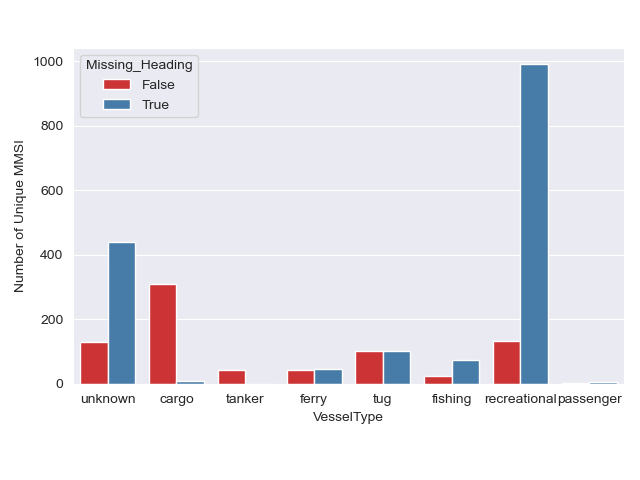
\includegraphics{Comparison_Type.png}
    \caption{The majority of vessels with missing heading are of type recreational and unknown which do not impact the analysis as these types are not considered.}
    \label{fig:missingtype}
    \forceversofloat
\end{figure*}
\begin{table}
    \centering
    \begin{tabular}{l l l l l l l }
     MMSI       & BaseDateTime      & LAT   & LON    & SOG          & COG \\
     \hline
     366709780  & 20170717 17:59:29 & 47.0  & -122.6 & 10           & 179 \\
     366709780	& 20170717 17:59:29 & 47.0  & -122.6 & 10           & 179 \\
     366709780	& 20170717 17:59:29 & 47.0  & -122.6 & \textbf{15}  & 179 \\
     \hline
    \end{tabular}
    \vspace{0.1in}
    \caption{Example of duplicate keys and data. All rows are removed from the data set.}
    \label{tab:dataDuplicate}
\end{table}
Each data point in the AIS data is identified by its MMSI and timestamp; this is called the primary key and must be unique across the entire data set. If two data points have the same primary key, either (1) one point is removed if all other fields match or (2) both points are removed if the other fields conflict. A simplified example is shown in Table \ref{tab:dataDuplicate}. Rows 1 and 2 are exact duplicates and result in row 2 being removed. Row 1 and row 3 have duplicate primary keys but conflicting SOG; rather than predict which one is correct using surrounding data, for simplicity, both row 1 and row 3 are removed. In the study data set, a negligible amount of data points are exact duplicates and no data points have a duplicate primary key with conflicting fields. 

}
\par{% bad MMSI
The MMSI is the unique identifier of the vessel. Valid MMSI numbers are 9 digits and start with three digits between 200 and 776. The first three digits are the country code and correspond to the ship's flag State. AIS devices come with default MMSI numbers that must be manually updated once upon AIS installation. The use of default MMSI numbers in AIS can result in several ships sharing the same MMSI. There are no invalid MMSIs in the study data set at this point in the cleaning process. 
}
\par{
Beyond faulty data, the MarineCadastre data contains a significant amount of data corresponding to vessels that are not moving, \ie{stop segments}. Stopped vessels are not navigating and cannot be involved in a collision.\sidenote{When a stopped vessel is struck, it is called an allision.} Moored and anchored vessels can be identified by their speed, AIS transmission interval, and navigation status. Figure \ref{fig:sog} shows that a majority of data points have a SOG close to zero. A vessel's speed over ground (SOG) may not be exactly 0 when stopped due to swaying. Ships with low speed are generally involved in mooring and/or being assisted by tugs. To retain data points related solely to navigating, all data points with a SOG under 3 knots are removed from the data set (68.7\% of the data set). 
}
\begin{figure*}
\begin{tabular}{c}
  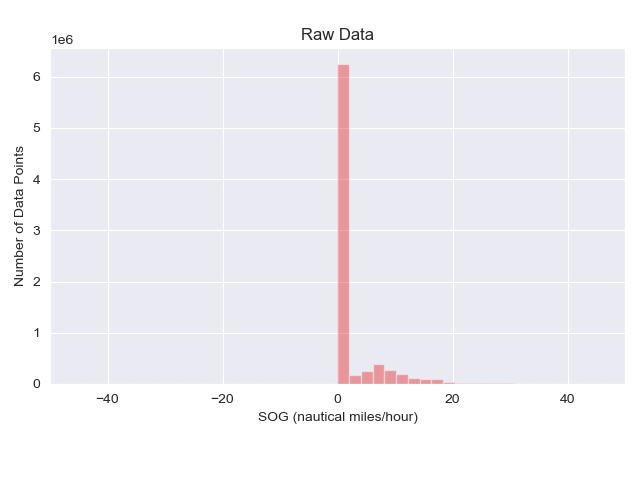
\includegraphics[width=0.95\textwidth]{Raw_SOG.png}\\
  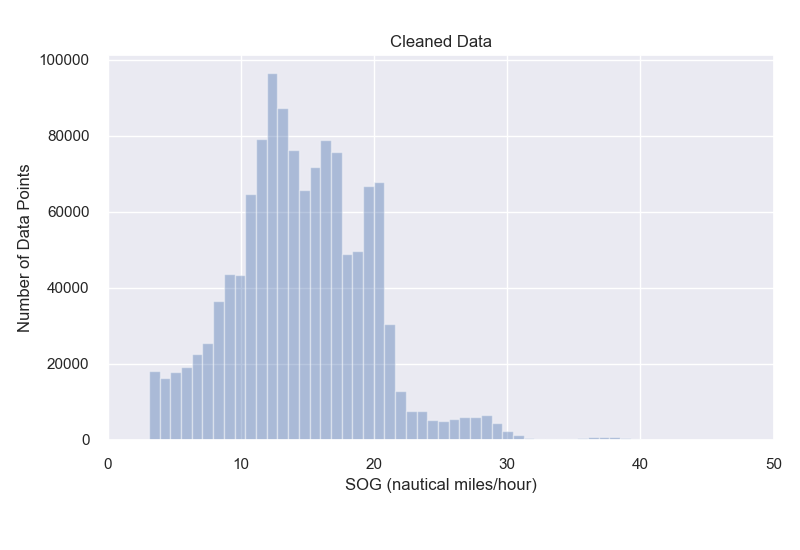
\includegraphics[width=0.95\textwidth]{Cleaned_SOG.png}\\
\end{tabular}
\caption{The majority of all data points correspond to a stopped vessel. When underway, most vessels operate at a SOG between 3 and 20 knots.}
\label{fig:sog}
\end{figure*}
\par{% interval
The time intervals between data transmissions are approximately three minutes if the vessel is stopped and one minute if the vessel is underway (AIS transmits more frequently, but NAIS data is sampled at one minute intervals). All data that was transmitted at an interval over 3 minutes is removed from the data set which accounts for 2.86\% of the data set.
}
\par{% status
The navigational status of the vessel (\eg{ underway using engine, moored, not under command}) can provide some additional information but should not be solely relied on. The status field is not complete; many vessels do not update this information or do not enter it at all. Vessels with an associated status of not under command, restricted maneuverability, engaged in fishing, power-driven vessel towing astern, reserved for future use, power-driven vessel pushing ahead, or towing alongside are discarded from the data set. These statuses correspond to non-normal navigation that are out of the scope of this dissertation. Their removal amounts to 2.18\% of the data set. The reason moored and anchored status are not excluded is because those are more commonly used and may not be updated once the vessel is underway. 
}
\par{% type
Vessels of type recreational, fishing, and tug are out of scope for this dissertation due to the type of activity the vessels of these types are generally engaged in. Fishing and recreational vessels do not consistently travel the shortest distance between an origin and destination while tugs are often  accompanying another vessel. Keeping only cargo, ferry, and tanker types reduces the data set by 39.2\%.
}

% -------------------------------------------------------------------------
\section{Data Processing}
\par{% creation of trips
The entire vessel trajectory for a given vessel may contain stops and/or data jumps and is not a usable form of the data. The trajectory must be broken into meaningful segments, trips, at break-points. Data for a single MMSI is sorted chronologically and segmented into trips based on time jumps greater than three minutes; any sparse trips --- those containing less than 20 data points --- are removed (23.32\% of the data set). In Table \ref{tab:trips}, Trip 2 begins with a time jump of 660 seconds (the \textcolor{red}{red} row). The time jumps have corresponding location jumps that are described by the displacement between successive locations. The \textcolor{blue}{blue} row demonstrates an unrealistic relationship between the time and location jumps.
}
\begin{table}
    \centering
    \begin{tabular}{l l l l l }
     MMSI       & Interval   & Trip  & Maximum Distance & Displacement  \\
     \hline
     \vdots     & \vdots & \vdots & \vdots & \vdots \\
     366709780	& 60    & 1 & 125 & 110 \\
     366709780	& 60    & 1 & 125 & 110 \\
     \textbf{\textcolor{red}{366709780}}	& \textbf{\textcolor{red}{660}}    & \textbf{\textcolor{red}{2}} & \textbf{\textcolor{red}{955}} & \textbf{\textcolor{red}{1150}} \\  
     366709780	& 60    & 2 & 150 & 110 \\ 
     \textbf{\textcolor{blue}{366709780}}	& \textbf{\textcolor{blue}{60}}    & \textbf{\textcolor{blue}{2}} & \textbf{\textcolor{blue}{150}} & \textbf{\textcolor{blue}{190}} \\    
     366709780	& 60   & 2 & 150 & 110 \\
     \vdots     & \vdots & \vdots & \vdots & \vdots \\
     \hline
    \end{tabular}
    \vspace{0.1in}
    \caption{The trajectory is first split into two trips based on Time Interval (red row). Then the displacement between consecutive points is compared with the maximum distance the vessel could have travelled given its reported SOG. The blue row is an example of unrealistic data.}
    \label{tab:trips}
    \forcerectofloat
\end{table}
\begin{table}
    \centering
    \begin{tabular}{l l l l l }
     MMSI       & Interval   & Trip  & Maximum Distance & Displacement  \\
     \hline
     \vdots     & \vdots & \vdots & \vdots & \vdots \\
     366709780	& 60    & 1 & 125 & 110 \\
     366709780	& 60    & 1 & 125 & 110 \\
     \textbf{\textcolor{red}{366709780}}	& \textbf{\textcolor{red}{660}}    & \textbf{\textcolor{red}{2}} & \textbf{\textcolor{red}{955}} & \textbf{\textcolor{red}{1150}} \\  
     366709780	& 60    & 2 & 150 & 110 \\ 
     \sout{366709780}	& \sout{60}    & \sout{2} & \sout{150} & \sout{190} \\  [-1.5ex]
     \hline \\[-1.5ex]
     \textbf{\textcolor{orange}{366709780}}	& \textbf{\textcolor{orange}{120}}    & \textbf{\textcolor{orange}{2}} & \textbf{\textcolor{orange}{300}} & \textbf{\textcolor{orange}{200}} \\
     \vdots     & \vdots & \vdots & \vdots & \vdots \\
     \hline
    \end{tabular}
    \caption{Because the orange row is within the expected ranges for Trip 2, it suggests that the row that is struck-out had bad GPS coordinates that resulted in an anomalous displacement.}
    \label{tab:trips2}
    \forcerectofloat
\end{table}
\par{
Within a single trip, the time between two consecutive positions and the SOG at the first position are used to calculate the maximum distance the vessel could have travelled between the two points. The displacement is the haversine distance between the two consecutive GPS coordinates that have been projected from WGS84 to UTM Zone 10N. If the displacement is larger than the maximum distance by more than 25\%, the data point is removed and the creation of trips is rerun; this step removes 1.4\% of the data set. The \textcolor{blue}{blue} row in Table \ref{tab:trips} has a displacement that is too large and is therefore removed from the data set. The time interval and distance fields are then recalculated (Table \ref{tab:trips2} \textcolor{orange}{orange} row). In this case, the time interval and displacement between the points just prior and just after the deleted row are within the expected ranges and Trip 2 remains in progress; if they were outside the expected ranges, Trip 3 would begin and Trip 2, consisting of only 2 data points, would be removed all together. Because the \textcolor{orange}{orange} row is within the expected ranges for Trip 2, it suggests that the row that is struck-out had bad GPS coordinates that resulted in an anomalous displacement.
}
\par{% round timestamps
Lastly, the datetime of the GPS position report in MarineCadastre data is sampled at one minute intervals. For ease of comparison, once the preprocessing of the data is completed, the timestamps are rounded to their nearest minute so that vessel positions can be compared at common timestamps. 
}
\par{% eda
Now that the data is cleaned we can take the first look at the maneuvers of interest: speed and heading changes (Figures \ref{fig:accel} and \ref{fig:alter}). The majority of data points have zero acceleration and small  alteration suggesting that mariners rarely make evasive maneuvers in the Puget Sound. Next, I construct the database from the data so I can relate these observed maneuvers to the presence of other vessels.
\begin{figure}
    \centering
    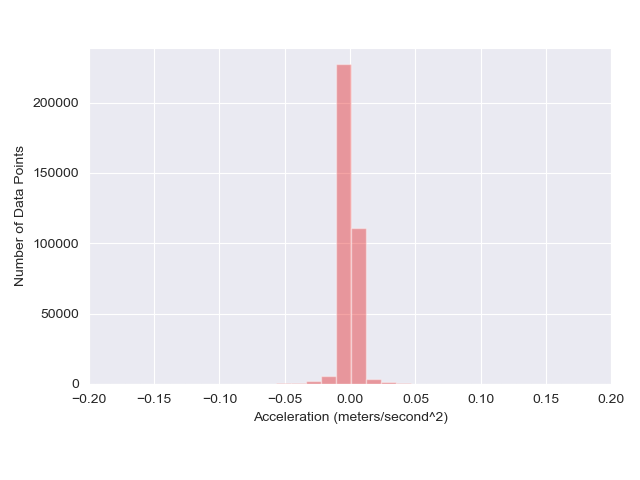
\includegraphics[width=1\textwidth]{Acceleration.png}
    \caption{The majority of all data points have little acceleration.}
    \label{fig:accel}
\end{figure}
\begin{figure}
    \centering
    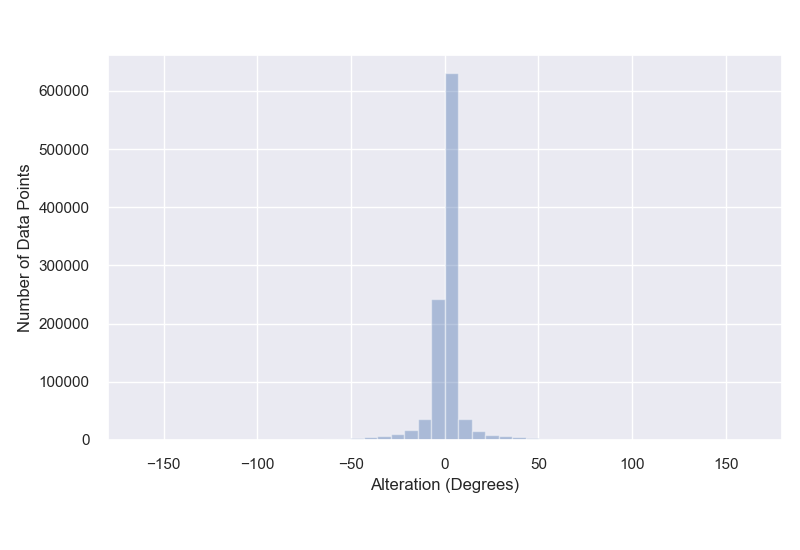
\includegraphics[width=1\textwidth]{Alteration_Degrees.png}
    \caption{The majority of all data points correspond to relatively constant heading.}
    \label{fig:alter}
\end{figure}
}
% --------------------------------------------------------------------
\section{Database Construction}
\par{% environment
The environmental data sets needed in the analysis are (1) traffic separation schemes, (2) shoreline, and (3) ferry terminal locations. Each data set contains spatial information in the form of a geometry; MultiPolygon for TSS, LineString for shoreline, and Point for ferry terminal locations. The data sets are loaded into separate tables in the same \textit{PostgreSQL} database. The geometry in each table is projected from its source coordinate reference system (CRS) to that in which the analysis takes place, EPSG:32610.
}
\par{% points
Next, the cleaned and processed data points are used to create the \mintinline{python}{points} table, with the spatiotemporal data stored as a \textit{PointM} data type using the \textit{PostGIS} extension, where M denotes a third dimension --- time --- in addition to the latitude and longitude. The other attributes stored in the \mintinline{python}{points} table include: MMSI, Trip, DateTime, LAT, LON, SOG, COG, Heading, Acceleration,  Alteration, Vessel Name, Vessel Type, Status, and Length. The ferry terminals table is used to assign terminals to points within one nautical mile of a terminal. The Traffic Separation Schemes table is used to mark each data point as being within or outside a TSS by performing a \mintinline{python}{ST_Contains(tss.geom, point,geom)} check. Figure \ref{fig:in_tss} shows that while cargo and tanker vessels spend a majority of time in and out of a TSS, ferries spend the majority of time outside of the traffic separation schemes.
\begin{figure}
    \centering
    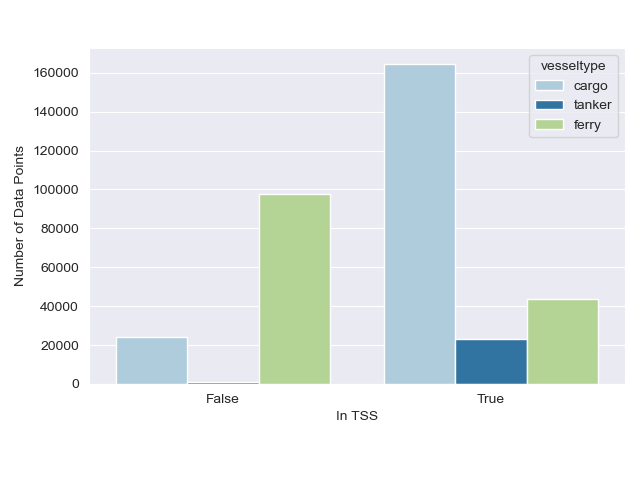
\includegraphics{TSS.png}
    \caption{The majority of ferry data points fall outside of a TSS; cargo and tanker data points are mostly within a TSS.}
    \label{fig:in_tss}
\end{figure}
}
\begin{figure*}
\begin{tabular}{cc}
  \includegraphics[width=85mm]{allTracks.png} &   
  \includegraphics[width=85mm]{cargoTracks.png} \\
(a) All & (b) Cargo \\[6pt]
 \includegraphics[width=85mm]{ferryTracks.png} &  
 \includegraphics[width=85mm]{tankerTracks.png} \\
(c) Ferry & (d) Tanker \\[6pt]
\end{tabular}
\caption{Most vessels keep to the traffic separation schemes; ferries have the most cross-TSS traffic.}
\label{fig:tracks}
\forcerectofloat
\end{figure*}
\begin{figure}
        \centering
    	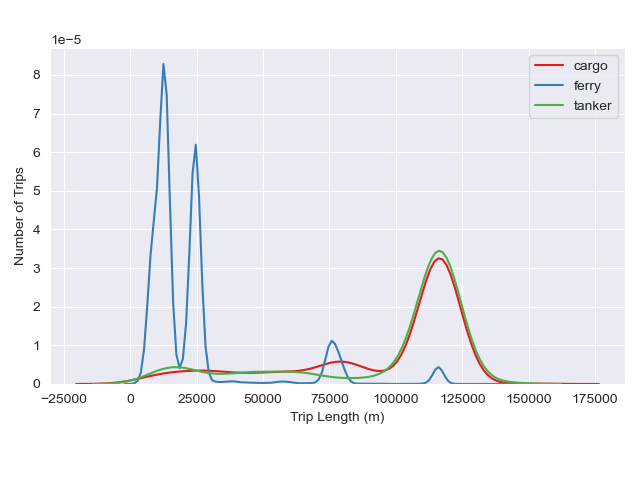
\includegraphics{Trip_Length.png}
	    \caption{The majority of trips are short ferry trips. The longer trips correspond to ships coming from the Pacific Ocean into Vancouver, B.C. or the south Puget Sound.}
    	\label{fig:tripLength}
    	\forcerectofloat
\end{figure}
\par{% tracks
Next, the \mintinline{python}{points} are used to generate a \mintinline{python}{tracks} table by first grouping \mintinline{python}{points} by MMSI and Trip, sorting chronologically, and then combining the result into the \textit{LineStringM} data type. These tracks are the trajectories that are used to construct encounters. The number of tracks in total is 4,542: 933 cargo tracks, 3,501 ferry tracks, and 108 tanker tracks. In Figure \ref{fig:tracks} you can clearly see the presence of the Strait of Juan de Fuca traffic separation scheme (reference Figure \ref{fig:straitTSS} for a clearer view of the TSS). The major ports in Washington State (Everett, Seattle, Tacoma) are visible in the far eastern portion of the cargo map. The cross-TSS routes of ferries can be seen in the East-West band between Coupeville and Port Townsend at the north end of the Puget Sound and the East-West band between Seattle and Bainbridge/Bremerton farther sougth. The distribution of trip lengths can be seen in Figure \ref{fig:tripLength}. The distance and duration of each track is calculated and stored in the table. If a ferry terminal is associated with the first point of a track, it is recorded as the trip's origin; similarly, if a ferry terminal is associated with the last point of a track, it is recoreded as the trip's destination.
}
\par{% CPA
Interactions between vessels are detected through the closest point of approach (CPA). If the CPA between two vessels' tracks exists, the interaction is saved to the \mintinline{python}{cpa} table. The CPA is calculated using the PostGIS \mintinline{python}{ST_ClosestPointOfApproach} function which returns the timestamp at which the CPA occurs and \mintinline{python}{ST_DistanceCPA} function which returns the distance between the two vessels at the CPA. Both functions require two LineStrings as input which is why the \mintinline{python}{tracks} table must be created as an intermediary table. The timestamp of the CPA is used to find the point in each vessel's track that corresponds to the CPA, \mintinline{python}{cpa_point_1} and \mintinline{python}{cpa_point_2}. A line is then drawn between these CPA points, \mintinline{python}{cpa_line}, and any interaction whose \mintinline{python}{cpa_line} crosses the shoreline, \mintinline{python}{ST_Intersects(cpa.cpa_line, shore.geom)} is removed from the \mintinline{python}{cpa} table. Lastly, any interaction with a CPA greater than four nautical miles is removed.
}
\par{
The \mintinline{python}{cpa} table only contains information about the closest point of approach. To get information about the vessels before and after the CPA, I must join \mintinline{python}{points} data to the \mintinline{python}{cpa} table. First, \mintinline{python}{point} data relating to \textit{ship 1} is left joined to \mintinline{python}{cpa} based on MMSI and where \mintinline{python}{points.DateTime} is between 10 minutes prior to the CPA and 20 minutes after the CPA. Next, \mintinline{python}{point} data relating to \textit{ship 2} is inner joined to the resulting table where its \mintinline{python}{points.DateTime} matches those already in the joined table. Interactions that have less than 10 data points prior to the CPA are removed from the analysis. Derived attributes are added in this step as well, including:
\begin{itemize}
    \item distance between ship 1 and ship 2 at each timestamp
    \item bearing between ship 1 and ship 2 at each timestamp
    \item difference in heading between ship 1 and ship 2 at each timestamp
    \item max course alteration for ship 1 and ship 2 during the encounter
    \item time to CPA 
    \item distance to CPA for each ship
    \end{itemize}
Figure \ref{fig:cpa} shows the distribution of CPA for various ship type pairings. For most ship type pairings there appear to be two modes, one corresponding to traffic within a single lane of the traffic separation scheme and one corresponding to traffic in opposite lanes of the TSS. Ferry-ferry interactions do not have a bi-model CPA distance distribution since ferries do not follow a TSS for a majority of their trips. The physical layout of the TSS therefore strongly influences the CPA distance. 
\begin{figure*}
    \centering
    \includegraphics{CPA.png}
    \caption{The mode of CPA distance around 2.5-3 nautical miles corresponds to traffic in opposite lanes of the TSS.}
    \label{fig:cpa}
\end{figure*}
}
\par{% classification
The interactions must then be classified as head-on, overtaking, or crossing as the applicable \textsc{colregs} depend on the encounter type. The encounter type is a function of the difference in heading between the vessels as shown in Table \ref{tab:encounter} and bearing. The classification of the encounter takes place before either vessel maneuvers and, therefore, before the closest point of approach. To observe the initial course difference and bearing between any two vessels, I take the first available concurrent observation of each vessel's course. Vessels traveling near each other while not actually passing are removed from the analysis by checking the beginning and final bearing between the vessels. In a head-on encounter, for instance, the bearing from \textit{ship 1} to \textit{ship 2} must cross either 90\textdegree or 270\textdegree to indicate that the vessels did indeed pass starboard-to-starboard or port-to-port. Table \ref{tab:encounterTypes} shows the breakdown by encounter type, vessel type, and whether either ship was in a TSS. Note that at this point not all interactions involve evasive maneuvers; they simply satisfy geometric definitions of encounters and are within four nautical miles of each other. Two ships in a head-on encounter with a passing distance of 4nm may feel that is a safe passing distance and make no evasive maneuvers. Most encounters involve a ferry with ferry-ferry crossing outside of the traffic separation scheme being the most common. Figure \ref{fig:cpaencounter} shows that head-on encounters have the smallest CPA; head-on encounters are mostly likely to involve two ferries and this ship type pairing is also likely to have a small CPA.
\begin{table}
\begin{tabular}{|l|l l|}
     \hline
        Encounter Type & Relative Heading  & Relative Bearing\\
        \hline
        \hline
        Head-On & $165 < \alpha < 195$  &  $\beta < 15$, \,  $\beta > 345$\\
        \hline
        Overtaking &  $\alpha < 15$, \,  $\alpha > 345$ &  $\beta < 15$, \,  $\beta > 345$, \\
                &                                       & $165 < \beta < 195$\\
        \hline
        Crossing & $15 < \alpha < 165$ &  $0 < \beta < 90$\\
                 & $195 < \alpha < 345$ &  $270 < \beta < 360$\\
        \hline
    \end{tabular}
    \vspace{.1in}
    \caption{The encounter type depends on the course difference and bearing between the two vessels.}
    \label{tab:encounter}
\end{table}
\begin{table}
\centering
\begin{tabular}{|l | l | l| l l | l l | l |}
\hline
          &          &          & Cargo &       & Ferry &       & Tanker\\
\hline
          &          & TSS   & F & T  & F & T  & T\\
\hline
\hline
\rowcolor{Gray}
Crossing  & Cargo    & F    & 1             & 4             & 14            & 3             & \textendash \\
\rowcolor{Gray}
          &          & T     & \textendash   & 7             & 18            & 10            & \textendash \\
          & Ferry    & F    & 5             & 13            & 216           & 26            & 1 \\
          &          & T     & 3             & 8             & 30            & 12            & \textendash\\
\rowcolor{Gray}
          & Tanker   & T     & \textendash   & 1             & \textendash   & \textendash   & \textendash\\
\hline
Head-on   & Cargo    & F    & \textendash   & 2             & \textendash   & 2             & \textendash\\
          &          & T     & 1             & 4             & 4             & 6             & 1 \\
\rowcolor{Gray}
          & Ferry    & F    & 1             & 5             & 34            & 6             & \textendash\\
\rowcolor{Gray}
          &          & T     & \textendash   & 3             & 4             & 3             & \textendash \\
\hline
Overtaking& Cargo    & F    & \textendash   & 1             & 2             & \textendash   & \textendash\\
          &          & T     & 1             & 11            & 2             & 5             & 1\\
\rowcolor{Gray}
          & Ferry    & F    & \textendash   & 1             & 35            & 6             & \textendash\\
\rowcolor{Gray}
          &          & T     & 1             & 8             & 2             & \textendash   & \textendash\\
          & Tanker   & T     & \textendash   & 1             &  \textendash  & \textendash &  \textendash\\
\hline
\end{tabular}
\vspace{0.2in}
\caption{Encounters by encounter type, vessel type, and whether vessel is in a TSS.}
\label{tab:encounterTypes}
\forcerectofloat
\end{table}

}
\par{% give way stand on
Next, the give-way and stand-on responsibilities must be assigned to the vessels in each encounter. In a head-on encounter, both vessels must give-way. In an overtaking encounter, the vessel that is astern of the other is the give-way and the vessel being overtaken is the stand-on vessel. In a crossing encounter, if \textit{ship 2} is at a bearing between 0 and 112.5 from \textit{ship 1}, then \textit{ship 1} is the give-way vessel and \textit{ship 2} is the stand-on vessel. 
}
\par{% 
\begin{marginfigure}
    \includegraphics{CPAEncounterType.png}
    \label{fig:cpaencounter}
    \caption{Encounter 'none' refers to interactions where ships are simply near each other but do not have a risk of collision. The CPA distance is smallest for head-on encounters which also corresponds in general to ferr-ferry encounters.}
\end{marginfigure}
The ship encounter information is now structured in a way that can be queried to answer this dissertation's research questions. Again, all code to generate the data used in this analysis is available at \url{https://github.com/mkrowell/phd}.
}
\section{Ship Domain}
\label{sec:regress}
\par{%
The ship domain is the area around a vessel the navigator keeps clear of other vessels and can be detected by observing the distance the ownship keeps between itself and target ships. Previous ship domain research has found that the distance tends to be larger on starboard than on port and larger ahead than astern; the bearings with a larger distance correspond to bearings at which the \textsc{colregs} instruct mariners to avoid passing. To characterize the local Puget Sound ship domain, I construct a linear regression with the distance between ownship and target ship as the dependent variable. The features of ship interactions that I believe may influence this distance are the vessel types of both ships; the bearing between the ownship and target ship; the speed over ground of both ships; and whether one, none, or both ships are in a traffic separation scheme. To estimate the ship domain distance I fit a linear regression of the following form:

\begin{multline*}
D_{ijt} = \beta_0 + \beta_1 sin(B_{ijt}) + \beta_2 cos(B_{ijt}) + \beta_3 TSS_{it} + \beta_4 TSS_{jt} + \\ \beta_5 TSS_{it} \times TSS_{jt} + \beta_6 S_{it} + \beta_7 S_{jt} + \lambda_i + \gamma_j + \\
\boldsymbol{\phi} sin(B_{ijt}) \times \mathbf{X_{ijt}} + \boldsymbol{\psi} cos(B_{ijt}) \times \mathbf{X_{ijt}}  + \epsilon_{ijt}
\end{multline*}
\begin{align*}
\text{where}~D_{ijt}    &= \text{distance from ship \textit{i} to ship \textit{j} at time \textit{t}}      \\
    B_{ijt}             &= \text{bearing from ship \textit{i} to ship \textit{j} at time \textit{t}}       \\
    TSS_{it}            &= \text{whether ship \textit{i} is in a TSS at time \textit{t}}          \\
    TSS_{jt}            &= \text{whether ship \textit{j} is in a TSS at time \textit{t}}          \\
    S_{it}              &= \text{speed over ground of ship \textit{i} at time \textit{t}}         \\
    S_{jt}              &= \text{speed over ground of ship \textit{j} at time \textit{t}}         \\
    \lambda_{i}         &= \text{fixed effect for vessel type of ship \textit{i}} \\
    \gamma_{j}         &= \text{fixed effect for vessel type of ship \textit{j}} \\
    \mathbf{X_{ijt}}    &= \begin{aligned}[t]
                            &\text{covariates matrix consisting of the indicators}\\
                            &\text{for ship \textit{i} and ship \textit{j} TSS belonging at  time \textit{t} and}\\
                            &\text{their interaction and ship \textit{i} and ship \textit{j} vessel types}\\
                        \end{aligned}  
\end{align*}
Ship \textit{i} refers to the ownship and ship \textit{j} refers to the target ship. The bearing is from ship \textit{i} to \textit{j}, and for the same pairing of ships there will be two observations with each ship appearing as the ownship in one and the target ship in the other. 
}
\par{% estimation
I estimate the parameters via Ordinary Least Squares regression using Python's \mintinline{python}{statsmodel}\cite{seabold2010statsmodels} package. The standard errors are clustered by MMSI and trip to account for correlated observations during an encounter. Using various sets of the independent variables as input to the predicted model, I can generate the conditional expectation of the distances. The scenarios of interest are:
\begin{enumerate}
    \item ship \textit{i} ferry in TSS, ship \textit{j} cargo in TSS
    \item ship \textit{i} ferry in TSS, ship \textit{j} ferry in TSS
    \item ship \textit{i} cargo in TSS, ship \textit{j} ferry in TSS
    \item ship \textit{i} cargo in TSS, ship \textit{j} cargo in TSS
    \item ship \textit{i} cargo in TSS, ship \textit{j} cargo out of TSS
\end{enumerate}
where speed is the average for the vessel type in all scenarios.
}
\section{Limitations}
\par{% missing influences
While the analyses conducted in the dissertation make use of a lot of AIS data, they still lack the complete picture of the maritime operating environment in the Puget Sound. Data left out of the analysis include vessels of other types (\eg{fishing, recreational}), weather and sea state information, and grounding hazards as well as non-observable information regarding any communication between vessels. The presence of vessels not included in the analysis as well as environmental factors may be influencing the observed behavior of in-analysis vessels. Including this additional information would follow a similar methodology as described here by expanding the database to include the desired information and would require more computing time and storage.
}



% -----------------------------------------------------------------------------
% RESULTS
% -----------------------------------------------------------------------------
\chapter{Results and Conclusions}
\par{% give way v stand on
The \textsc{colregs} assign responsibilities to each vessel when they are in an overtaking, head-on, and crossing situation. The stand-on vessel has the responsibility to continue with its current speed and course. The other vessel, the give-way vessel, should take action to avoid a collision. The give-way vessel would like to make the smallest deviation necessary to prevent collision, but its action must be, according to Rule 8, made early and large enough to be apparent to the stand-on vessel.\cite{USCG} Taking action as the stand-on vessel is only permitted when it becomes apparent that the give-way vessel is not taking appropriate action.
}
\par{% minimal interference
The \textsc{colregs} assert minimal authority over the give-way vessel's choice of evasive maneuver. The navigator is free to choose whether to alter course, speed, or both and to what degree; when to begin the maneuver; the minimum acceptable passing distance; and when to return to the original course and speed. Two restrictions on this discretion are (1) in a head-on encounter, where both ships are to alter course to starboard for a port-to-port passing and (2) in a crossing encounter, where the give-way vessel is to avoid passing ahead of the stand-on vessel.\cite{Plant}
}
\par{% rigid give way stand on designation
The discretion granted by the \textsc{colregs} when deciding an appropriate collision-avoidance maneuver gives way to rigidity when deciding which vessel is to give way and which is to stand on. This determination is based on the geometry of the encounter (see Figure \ref{fig:colregpic}): 
\begin{itemize}
    \item the overtaking vessel gives way to the vessel being overtaken;
    \item the vessel with the other to her starboard gives way to a crossing vessel; 
    \item and both vessels give way to each other in a head-on encounter.
\end{itemize} The geometry-based algorithm does not allow the speed and maneuverability of the vessels to enter into the decision. The strict assignment of give-way vessel can be termed a \textit{regulation} and the indistinct direction to give-way, a \textit{rule}. Regulations are a form of explicit, externally applied control; its text completely defines its interpretation. The text of a rule is ambiguous and requires observing the system it refers to in order to interpret its meaning. The navigator must rely on an interpretation of the rules that is consistent with what other mariners would expect of him. The ordinary practice of seamen can be thought of as the agreed upon interpretation of the ambiguous rules --- the patterns of behavior --- that, when necessary, supersedes the regulations. What appears to be a deviation from the \textsc{colregs}, may in fact be ``the use of informal, group rules, which are seen as violations by those on the outside, but as skilled adaptations by those on the inside.''\cite{Hale}
}
\par{% infer rules
Research problem 1 of this dissertation is ``How do mariners in the Puget Sound interpret the \textsc{colregs}?'' 
The key phrases that are up for interpretation are:
\begin{itemize}
    \item passing at a safe distance
    \item any action to avoid collision shall be\ldots made in ample time\ldots any alteration of course and/or speed to avoid collision shall\ldots be large enough to be readily apparent to another vessel observing visually or by radar
    \item as soon as it becomes apparent to her that the vessel required to keep out of the way is not taking appropriate action
\end{itemize}
Parts of the \textsc{colregs} that are not up for interpretation are the rules to:
\begin{itemize}
    \item give way and pass port-to-port in head-on encounters
    \item to give way to the vessel on your starboard and avoid passing ahead of the vessel in a crossing encounter
    \item cross traffic separation schemes at near-90 degree angles relative to the traffic separation scheme.
 \end{itemize}
Observing violations of these rules provides answers to research problems 2 "Are informal rules being followed?" and research problem 3 "What is the nature and frequency of \textsc{colregs} violations.
}
\section{Safe Passing Distance}
\par{%
Rule 8c of the \textsc{colregs} states that:
\begin{quotation}
Action taken to avoid collision with another vessel shall be such as to result in passing at a safe distance. 
\end{quotation}
The ship domain as described in Section \ref{sec:shipdomain} is the lower bound of what mariners consider a safe passing distance. The population of mariners operating in Puget Sound is a mix between local ferry captains and international cargo vessel crews. In addition to familiarity with the area, ferry vessels have smaller, more maneuverable vessels. For these reasons, I expected to observe ferries maintaining a smaller passing distance than cargo vessels. Querying the bearing and distance from the ownship to the target ship from the \mintinline{python}{encounters} table and plotting the results generates Figure \ref{fig:shipDomainResutls}. Each subplot represents a different pairing of vessel types between the ownship and target ship. Take the \textit{target ship ferry} - \textit{ownship cargo} pairing for example, the center of the plot (r=0) represents a static cargo vessel and each point surrounding the center is an observation of a ferry at the bearing and distance from the cargo vessel that it was observed. Due to the restricted nature of the Strait of Juan de Fuca and Puget Sound and the proximity of traffic separation schemes, vessels are required to pass closer to one another than they would in the open sea; to increase readability, Figure \ref{fig:shipDomainResutls} shows target ships that were within two nautical miles of the ownship. In each plot, the blue points correspond to target vessels that are observed in a traffic separation scheme, and the red points correspond to target vessels observed outside a traffic separation scheme.
\begin{figure*}
    \centering
    \textbf{Distance versus Bearing}\par\medskip
    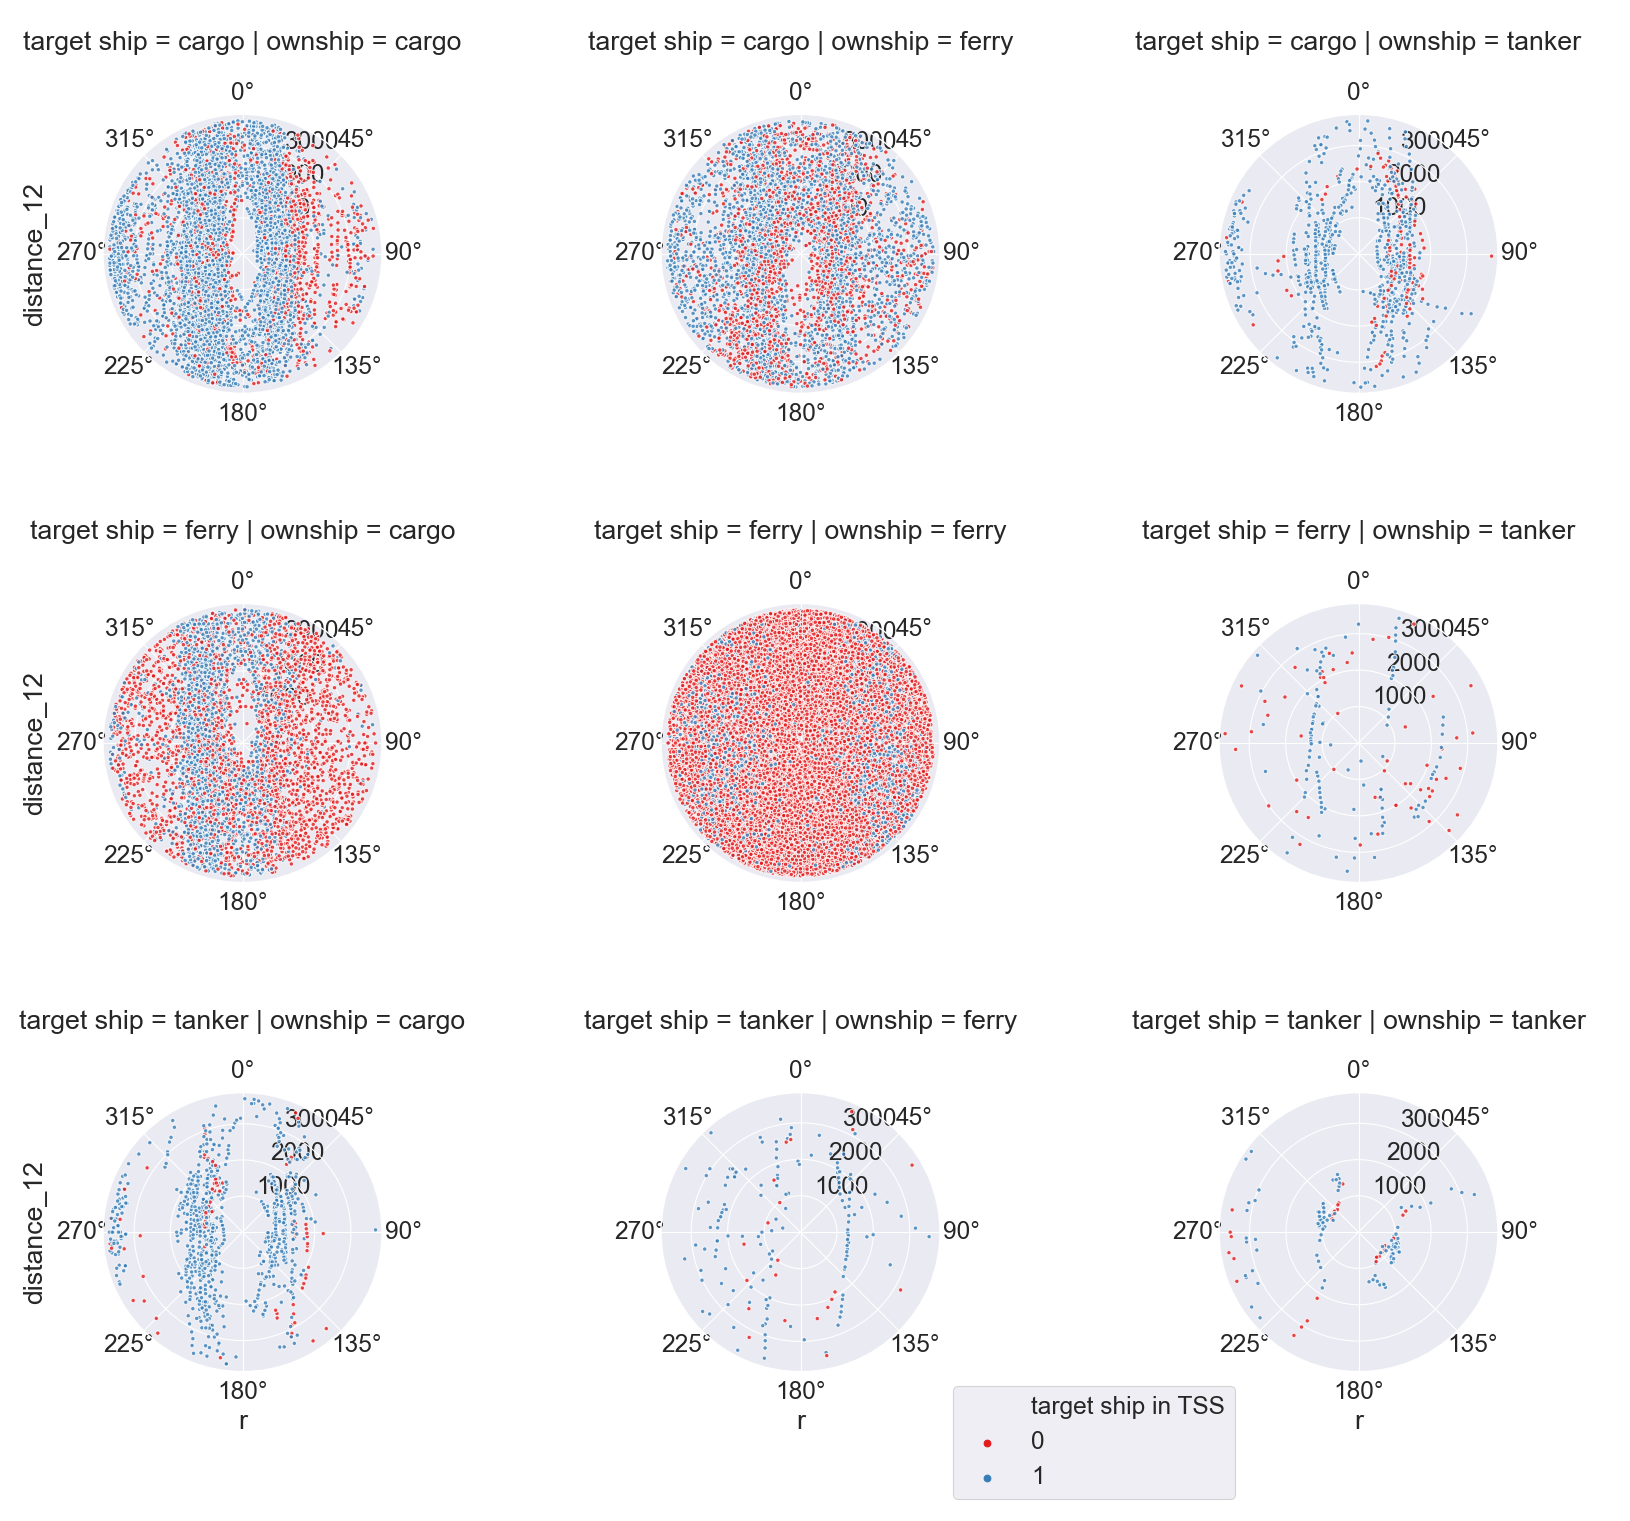
\includegraphics{Ship_Domain_1.png}
    \caption{Bearing and distance for all encounter types and all areas of the Puget Sound with distance less than 2nm. Blue dots are in a TSS; red dots are not.}
    \label{fig:shipDomainResutls}
\end{figure*}
}
\par{% ferry-ferry
The first plot that stands out in Figure \ref{fig:shipDomainResutls} is the \textit{target ship ferry} - \textit{ownship ferry} pairing. The plot area is almost totally covered and mostly in red; this shows (1) the large number of ferry-ferry passings, (2) that the majority of them take place outside the traffic separation schemes, and (3) the safe passing distance for this pairing is relatively small. Another plot that stands out is the \textit{target ship cargo} - \textit{ownship cargo} pairing. In contrast to the ferry-ferry plot, the majority of passings take place within a traffic separation scheme (blue dots) which accounts for the bands of points to the port and starboard. The traffic separation schemes impose order on vessels traveling in the same and opposite directions by separating vessels into ``lanes,'' with a separation zone in between. From this I can conclude that cargo vessels in the Puget Sound make use of the traffic separation schemes. 
}
\par{%
Turning my attention to vessel pairings of different types, the \textit{target ship cargo} - \textit{ownship ferry} and \textit{target ship ferry} - \textit{ownship cargo} have complementary plots. In the \textit{target ship ferry} - \textit{ownship cargo} plot, I observe a buffer area ahead of the cargo vessel that has relatively few observations of ferry target vessels. In the \textit{target ship cargo} - \textit{ownship ferry} plot, I observe the opposite, with a buffer area astern of the ferry that has relatively few observations of cargo target vessels. Additionally the ratio of red to blue points appears to be opposite. This suggests that ferries avoid passing ahead of cargo vessels.
}
\par{% regression
From these plots, I hypothesize that bearing to target ship, vessel types, and whether one, both, or none of the vessels are in a traffic separation scheme influence the distance from the ownship to the target ship. The results of the ship domain regression analysis described in the Section \ref{sec:regress} is shown in the table below.
\vspace{0.1in}
\begin{fullwidth}
\begin{center}
\begin{tabular}{llll}
\toprule
\textbf{Dep. Variable:}       &   distance\_12   & \textbf{  R-squared:         } &      0.180   \\
\textbf{Model:}               &       OLS        & \textbf{  Adj. R-squared:    } &      0.180   \\
\textbf{Method:}              &  Least Squares   & \textbf{  F-statistic:       } &      248.4   \\
\textbf{Date:}                & Sat, 30 May 2020 & \textbf{  Prob (F-statistic):} &      0.00    \\
\textbf{Time:}                &     15:23:58     & \textbf{  Log-Likelihood:    } & -6.5667e+05  \\
\textbf{No. Observations:}    &       67056      & \textbf{  AIC:               } &  1.313e+06   \\
\textbf{Df Residuals:}        &       67030      & \textbf{  BIC:               } &  1.314e+06   \\
\textbf{Df Model:}            &          25      & \textbf{                     } &              \\
\bottomrule
\end{tabular}
\begin{tabular}{lcccccc}
                              & \textbf{coef} & \textbf{std err} & \textbf{z} & \textbf{P$> |$z$|$} & \textbf{[0.025} & \textbf{0.975]}  \\
\midrule
\textbf{const}                &    5120.9747  &      319.617     &    16.022  &         0.000        &     4494.537    &     5747.412     \\
\textbf{type\_1\_ferry}       &    -419.5294  &      186.939     &    -2.244  &         0.025        &     -785.923    &      -53.136     \\
\textbf{type\_1\_tanker}      &     347.3420  &      757.388     &     0.459  &         0.647        &    -1137.110    &     1831.794     \\
\textbf{type\_2\_ferry}       &    -225.9696  &      187.348     &    -1.206  &         0.228        &     -593.166    &      141.227     \\
\textbf{type\_2\_tanker}      &     444.2651  &      832.260     &     0.534  &         0.593        &    -1186.935    &     2075.465     \\
\textbf{tss\_1\_True}         &     460.1361  &      154.333     &     2.981  &         0.003        &      157.649    &      762.623     \\
\textbf{tss\_2\_True}         &     483.7138  &      138.287     &     3.498  &         0.000        &      212.676    &      754.752     \\
\textbf{tss\_both\_True}      &    1073.5515  &      232.102     &     4.625  &         0.000        &      618.640    &     1528.463     \\
\textbf{bearing\_12\_sin}     &     114.0510  &      365.306     &     0.312  &         0.755        &     -601.935    &      830.037     \\
\textbf{bearing\_12\_cos}     &   -1836.9543  &      141.225     &   -13.007  &         0.000        &    -2113.751    &    -1560.158     \\
\textbf{sog\_1}               &      55.0582  &        8.911     &     6.178  &         0.000        &       37.592    &       72.524     \\
\textbf{sog\_2}               &      42.9914  &        8.610     &     4.993  &         0.000        &       26.116    &       59.867     \\
\textbf{type\_1\_ferry\_sin}  &      41.1128  &      271.461     &     0.151  &         0.880        &     -490.941    &      573.166     \\
\textbf{type\_1\_tanker\_sin} &     198.5102  &     1055.755     &     0.188  &         0.851        &    -1870.731    &     2267.752     \\
\textbf{type\_2\_ferry\_sin}  &     310.0832  &      270.071     &     1.148  &         0.251        &     -219.246    &      839.412     \\
\textbf{type\_2\_tanker\_sin} &     488.3426  &     1189.639     &     0.410  &         0.681        &    -1843.306    &     2819.991     \\
\textbf{tss\_1\_True\_sin}    &   -1185.6063  &      213.580     &    -5.551  &         0.000        &    -1604.215    &     -766.998     \\
\textbf{tss\_2\_True\_sin}    &    -210.0436  &      201.877     &    -1.040  &         0.298        &     -605.716    &      185.629     \\
\textbf{tss\_both\_True\_sin} &    2446.6064  &      373.159     &     6.556  &         0.000        &     1715.228    &     3177.985     \\
\textbf{type\_1\_ferry\_cos}  &     301.1415  &       96.500     &     3.121  &         0.002        &      112.006    &      490.277     \\
\textbf{type\_1\_tanker\_cos} &     457.3471  &      128.090     &     3.571  &         0.000        &      206.295    &      708.400     \\
\textbf{type\_2\_ferry\_cos}  &     301.3079  &       98.885     &     3.047  &         0.002        &      107.497    &      495.119     \\
\textbf{type\_2\_tanker\_cos} &       5.8585  &      175.110     &     0.033  &         0.973        &     -337.350    &      349.067     \\
\textbf{tss\_1\_True\_cos}    &    -517.8695  &      136.847     &    -3.784  &         0.000        &     -786.084    &     -249.655     \\
\textbf{tss\_2\_True\_cos}    &    -325.2054  &      146.896     &    -2.214  &         0.027        &     -613.117    &      -37.294     \\
\textbf{tss\_both\_True\_cos} &    -310.4683  &      195.778     &    -1.586  &         0.113        &     -694.186    &       73.250     \\
\bottomrule
\end{tabular}
\begin{tabular}{llll}
\textbf{Omnibus:}       & 3336.757 & \textbf{  Durbin-Watson:     } &    0.619  \\
\textbf{Prob(Omnibus):} &   0.000  & \textbf{  Jarque-Bera (JB):  } & 4171.963  \\
\textbf{Skew:}          &   0.514  & \textbf{  Prob(JB):          } &     0.00  \\
\textbf{Kurtosis:}      &   3.659  & \textbf{  Cond. No.          } &     390.  \\
\bottomrule
\end{tabular}
\end{center}

Warnings: \newline
 [1] Standard Errors are robust to cluster correlation (cluster)
\end{fullwidth}
}
\newpage
\par{%
Conducting an f-test on the features of interest shows that all are of statistical significance.
\begin{tabular}{lllrr}                                                                             
\toprule                                                                                            
 Feature &                 F Value &                 P Value &  DF Denom &  DF Num \\          
\midrule                                                                                            
   type\_1 & 5.239 &  2.302e-05 &      1968 &     6.0 \\          
   type\_2 &    2.7541 &    0.0114 &      1968 &     6.0 \\          
    TSS &  19.056 &   7.714e-31 &      1968 &     9.0 \\           
  bearing &   355.764 &                     0.0 &      1968 &    16.0 \\           
\bottomrule                                                                              
\end{tabular}                                       
}
\vspace{0.1in}
\par{% features
By plugging different scenarios into the estimated model, I can generate the conditional mean of the ship domain distance under various circumstances. The scenarios consist of choosing a vessel type for each ship and whether each ship is in a traffic separation scheme. Using the average speed for the vessel type and calculating the average distance at each bearing $[0, 360)$ for the scenarios listed below yields the plot of ship domains in Figure \ref{fig:domainResultsRegress}:
\begin{enumerate}
    \item ship \textit{i} ferry in TSS, ship \textit{j} cargo in TSS
    \item ship \textit{i} ferry in TSS, ship \textit{j} ferry not in TSS
    \item ship \textit{i} cargo in TSS, ship \textit{j} ferry in TSS
    \item ship \textit{i} cargo in TSS, ship \textit{j} cargo in TSS
    \item ship \textit{i} cargo out of TSS, ship \textit{j} cargo out of TSS
    \item ship \textit{i} ferry out of TSS, ship \textit{j} cargo in TSS
\end{enumerate}
\begin{figure*}
    \centering
    \includegraphics{RegressionPlot.png}
    \caption{The observed ship domains appear larger on the starboard and aft of the ship.}
    \label{fig:domainResultsRegress}
\end{figure*}
The larger overall ship domains correspond to Scenarios 1, 3, and 4 where both ships are in a traffic separation scheme. The ship domains for these scenarios also have a larger distance on starboard than port. Port-to-port passings may take place at smaller distances since both ships are in their dedicated lane and the risk of collision is low. The smaller ship domains correspond to Scenarios 2, 5, and 6 where at least one ship is not in a TSS.  I can conclude therefore that the traffic separation schemes are successful at separating traffic.
}
\section{Readily Apparent Alterations}
\par{Rule 8a and 8b of the \textsc{colregs} states that:
\begin{quotation}
Any action taken to avoid collision shall be taken in accordance with the Rules of this Part and shall, if the circumstances of the case admit, be positive, made in ample time and with due regard to the observance of good seamanship. Any alteration of course and/or speed to avoid collision shall, if the circumstances of the case admit, be large enough to be readily apparent to another vessel observing visually or by radar; a succession of small alterations of course and/or speed should be avoided.
\end{quotation}
Identifying large evasive maneuvers proved difficult; large course alterations were associated with turning points in routes as vessels made their way to and from ports rather than collision-avoidance. One explanation for why so few encounters occur and do not include apparent alterations could be that ferry captains can observe on AIS that a cargo vessel is in the TSS before leaving the ferry terminal. If a cargo vessel will be nearby during the ferry crossing, ferries take a slightly arcing route across the TSS to pass astern of the cargo vessel rather than beginning on a direct route and making a large course alteration in the middle of the TSS.
}
\par{%
To investigate this hypothesis, I took the ferries traveling between Seattle and Bainbridge and compared their route characteristics between when they were encountering another ferry (319 encounters) and when they were encountering a cargo vessel (51 encounters). The length and duration plots in \ref{fig:tripChar} show that ferry trips are longer in length and duration when the ferry is encountering a cargo vessel as compared to a ferry vessel. Plot (c) shows the straightness index, which is the displacement of the trip divided by the length. If the trip is straight across, the straightness index would be 1. The figure shows that when the target vessel is a cargo vessel, the straightness of the route slightly decreases.
}
\begin{figure*}
\begin{tabular}{cc}
  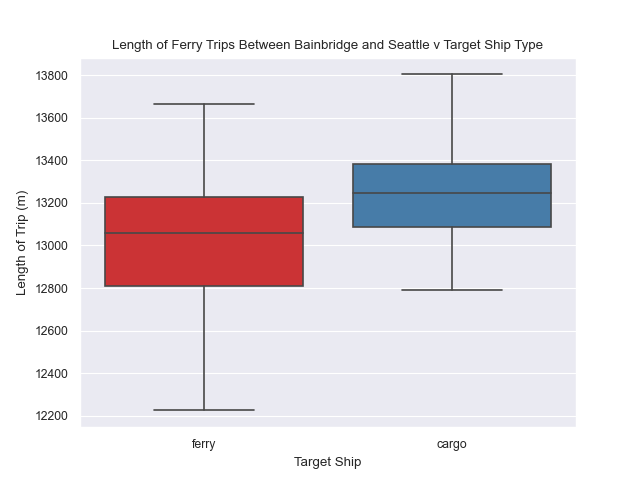
\includegraphics[width=85mm]{lengthTrip.png}&   
  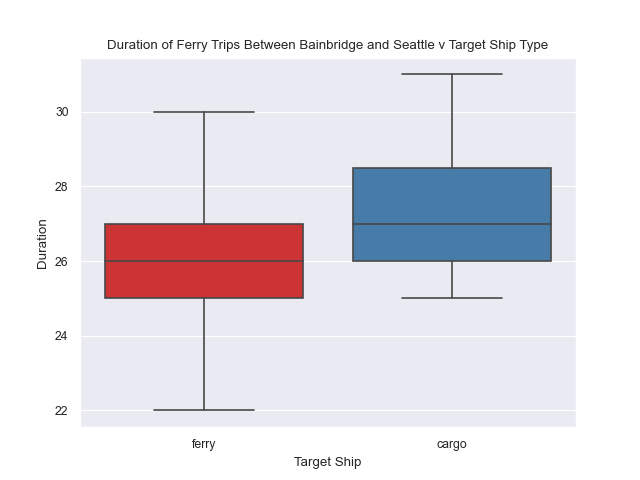
\includegraphics[width=85mm]{durationTrip.png} \ \\
(a) Length & (b) Duration \\[6pt]
 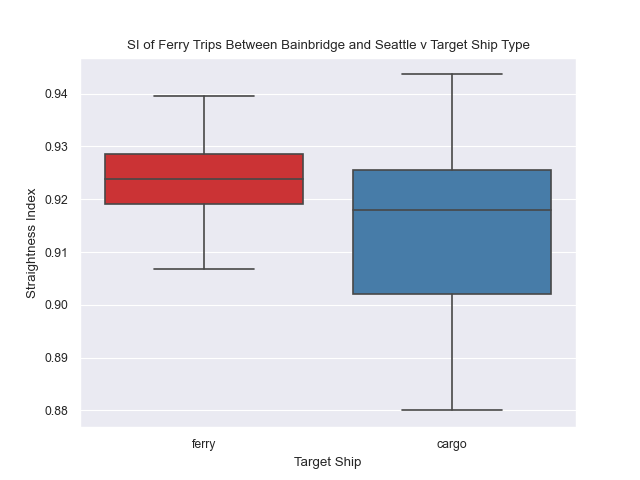
\includegraphics[width=85mm]{si.png} &  
 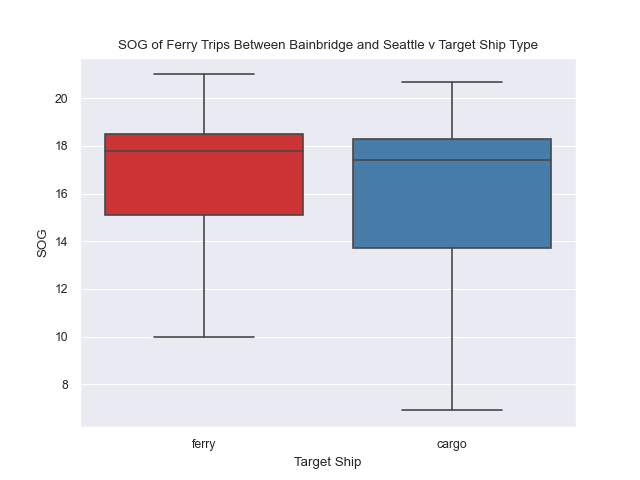
\includegraphics[width=85mm]{sogTrip.png} \\
(c) Straightness & (d) Speed \\[6pt]
\end{tabular}
\caption{Most vessels keep to the traffic separation schemes; ferries have the most cross-TSS traffic.}
\label{fig:tripChar}
\forcerectofloat
\end{figure*}
\par{%
This supports the hypothesis that the crossing ferry slightly alter their route across the TSS to avoid cargo vessels. This type of collision-avoidance does not show up in the data as large course or speed alterations. The stand-on and give-way cargo vessels show no difference in behavior; the appropriate stand-on behavior of the ferry is to avoid the give-way ferry. International cargo vessels will have a local pilot on-board who can inform them of this informal ferry rule.
}
\section{Traffic Separation Scheme Crossing Angle}
\par{
Rule 10 of the \textsc{colregs} specifies that: 
\begin{quotation}
A vessel shall, so far as practicable, avoid crossing traffic lanes but if obliged to do so shall cross on a heading as nearly as practicable at right angles to the general direction of traffic flow. 
\end{quotation}
Again, the rule is intended to make ships crossing the traffic separation scheme distinct from ships which are joining the traffic separation scheme. Observing Washington State Ferry (WSF) crossings of the traffic separation schemes between Seattle on the east and Bainbridge and Bremerton on the west using the approach set out in the methodology, shows a bi-modal distribution of crossing angles (Figure \ref{fig:entrance_angle_his}). The location of the TSS entrances are mapped in Figure \ref{fig:anlge}, where blue points correspond to entrance angles between 80 and 90 degrees relative to the TSS and red points correspond to entrance angles between 0 and 80.
\begin{figure*}
    \centering
    \includegraphics[width=1\textwidth]{TSS_Entrance_Angle.png}
    \caption{Washington State Ferries' relative angle to traffic separation scheme.}
    \label{fig:entrance_angle_his}
\end{figure*}
\begin{figure*}
    \centering
    \includegraphics{entrance_angle.png}
    \caption{Points where a WSF entered a traffic separation scheme.}
    \label{fig:anlge}
    \forceversofloat
\end{figure*}
}
\par{
The mode near 90 corresponds to ferries traveling between Seattle and Bainbridge where the ferry route already crosses the traffic separation scheme at a near-90 degree angle (Figure \ref{fig:bainbridge}). The mode near 70 corresponds to ferries traveling between Seattle and Bremerton where the ferry route is at a non-90 degree angle to the TSS (Figure \ref{fig:bremerton}). Because all Seattle-Bremerton ferries crossed the TSS at a non-90 degree angle this behavior is not considered a violation but rather an informal rule. An explanation for why this informal rule has not caused a safety concern could be that the distinct WSF vessels along with their AIS information is enough information for other vessels to know that the ferries are following a known route across the TSS and not joining the TSS. 
\begin{figure*}
    \centering
    \includegraphics{angle90.png}
    \caption{Example Seattle-Bainbridge ferry route that crosses the TSS at a relative 90 degree angle.}
    \label{fig:bainbridge}
\end{figure*}
\begin{figure*}
    \centering
    \includegraphics{angleBad.png}
    \caption{Example Seattle-Bremerton ferry route that crosses the TSS at a relative non-90 degree angle.}
    \label{fig:bremerton}
\end{figure*}

}
\newpage
\section{Starboard-Starboard Head-On Passings}
\begin{marginfigure}
    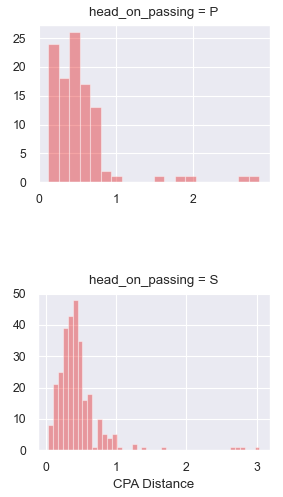
\includegraphics{headonCPA.png}
    \caption{The does not appear to be a difference in port-port and starboard-starboard CPA distance.}
\end{marginfigure}
\par{
The \textsc{colregs} require port-to-port passings in head-on encounters. Looking at head-on encounters with a CPA of two nautical miles or less (this is to remove the head-on encounters that appear at larger distances due to traffic in the TSS), 40\% are port-to-port while 60\% are starboard-to-starboard. Investigating the starboard-to-starboard passings (Figure \ref{fig:head_on_encounters}), I found that the majority correspond to ferry-ferry passings. Ferries have known routes and a known population of navigators. Some of the known routes require a starboard-to-starboard passing on occasion. For example, the Seattle-Bainbridge route is north of the Seattle-Bremerton route; when one ferry is pulling into Seattle from Bainbridge while another is pulling out of Seattle to Bremerton, this will occur starboard-to-starboard. 
}
\par{
The other starboard-to-starboard passings almost always have one vessel in the TSS and the other vessel outside the TSS. The vessel in the TSS is expected to continue in the TSS and may not be able to maneuver outside the TSS; the vessel outside the TSS should not enter the TSS in the wrong direction to force a port-to-port passing.
\begin{figure}
    \centering
    \includegraphics{HO.png}
    \caption{The majority of starboard-to-starboard head-on passings are attributed to ferries.}
    \label{fig:head_on_encounters}
\end{figure}
\begin{figure}
    \centering
    \includegraphics{HO_Split.png}
    \caption{When one vessel is in the TSS and the other is not, the informal rule is to pass starboard-to-starboard and not force a port-to-port.}
    \label{fig:my_label}
\end{figure}
}
\newline
\section{Conclusions}
\par{%
What this dissertation has discovered is that the Puget Sound is a safe maritime environment regarding ferry and cargo vessels. The traffic separation schemes limit the number of encounters and keep passing ships at a safe distance. The Washington State Ferries appear to avoid a risk of collision with cargo vessels by delaying their crossing of the traffic separation schemes in order to pass astern of cargo vessels regardless of their give-way status. They do this by slight altering their course and speed rather than making noticeable alterations. Outside of the informal rules, no violations of the \textsc{colregs} were discovered. The main conclusion from this research are:
\begin{enumerate}
        \item Cargo vessels use the traffic separation schemes to maintain safe passing distance.
        \item No cargo vessel was found to alter course or speed in response to the presence of a ferry vessel.
        \item Ferries cross the traffic separation scheme at an angle that aligns with their route rather than at a strictly 90 degree angle.
        \item Ferries make small alterations to avoid encountering cargo vessels.
        \item Passing distances are slightly larger on starboard than on port.
        \item Ferries are most likely to pass starboard-to-starboard due to the layout of their routes; other starboard-to-starboard head-on encounters occur when one vessel is traveling in the TSS and the other is not.
\end{enumerate}
}
\par{%
}


% \par{% overview summary of characteristics
% Seattle has a very good safety culture. In 2014, it had only 4 reported incidents of type collision, allision, or grounding compared to the lower Mississippi which had 59
% \sidenote{Puget Sound Partnership. (2014). VTRA 2010 Final Report. \url{https://www.seas.gwu.edu/\~dorpjr/tab4/publications\_VTRA\_Update\_Reports.html}} 
% \sidenote{USCG. (1973). Increased Safety through Vessel Traffic Systems. \textit{Proceedings of the Marine Safety Council.}, \textbf{30}, 12. pp. 251-257.} 
% \sidenote{USCG. (2016). Coast Pilot 7 Pacific Coast: California, Oregon, Washington, Hawaii, and Pacific Islands.} The need to direct vessels is not common, occurring, on average, 40 times a year.\sidenote{USCG. (2016). Coast Guard Intervenes in Dangerous Vessel Traffic in Puget Sound. \url{http://www.uscgnews.com/go/doc/4007/2858366/Coast-Guard-intervenes-in-dangerous-vessel-traffic-in-Puget-Sound}}  
% }


% =================================================================
% APPENDICES
% ==================================================================
% \begin{appendices}
% \appendixpage
% \noappendicestocpagenum
% \addappheadtotoc

% \end{appendices}


% =================================================================
% REFERENCES
% ==================================================================
\backmatter


\bibliographystyle{plainnat}
\bibliography{references.bib}

\end{document}
